%% draft+final=finaldraft (no todos, but draft note at foot of page)
\documentclass[%
    draft, % comment draft to remove draft imprint at page foot
    %final, % give final when done. Overwrites draft. Removes todos.
    11pt,
    a4paper
    %fleqn, %
    %openany %%chapter on right and left pages (no cleardoublepage)
]
{memoir}

%% Prevents figure and table placements in random locations.
\usepackage{float}

\usepackage{hhline}

%% define control flags
\usepackage{ifthen}
\newboolean{printVersion}

\setboolean{printVersion}{false} % do not use colored links for print



\usepackage{lipsum}

%%%%%%%%%%%%%%%%%%%%%%%%%%
%% TOC space settings
%%%%%%%%%%%%%%%%%%%%%%%%%%
\setpnumwidth{3em}
\setrmarg{4em}


%%%%%%%%%%%%%%%%%%%%%%%%%%
%% floating environments
%%%%%%%%%%%%%%%%%%%%%%%%%%
\usepackage[final]          %w/o option final: no images in document-draft-mode
             {graphics}		% einbinden von graphiken

%\usepackage{caption}  %% not needed with documentclass memoir
\usepackage{subcaption} % neue subfigure-Umgebung %% should probably not be used with memoir: generates warning

%\usepackage[section]{placeins} %% \FloatBarrier

%% setup caption style (\usepackage{caption} w/o documentclass memoir)
\captionsetup[figure]{  labelfont       = {bf,color=captionCatergoryColor},
                        textfont        = {it,color=captionTextColor},
                        justification   = raggedright,
                        singlelinecheck = false,
                        position        = bottom,
                        format=hang
                        }
\captionsetup[table]{   labelfont       = {bf,color=captionCatergoryColor},
                        textfont        = {it,color=captionTextColor},
                        justification   = raggedright,
                        singlelinecheck = false,
                        position        = top,
                        format          = hang
                        }
%\captionsetup[table]{skip=7pt} %% mehr platz zwischen tabelle und caption

% move Text to Image. 1ex ~1 line of Text
% unfortunately: also valid for subcaptions.
%\setlength{\belowcaptionskip}{0ex}

% define how much text shall be on same page with large images
%% standard seems to be 0.20 --> 20%
%\renewcommand{\textfraction}{0.01}


%% Durchgängige Nummerierung von Figures und Tables:
%\usepackage{chngcntr}
%\counterwithout{figure}{chapter}
%\counterwithout{table}{chapter}


%define common figure sizes for subfigures
% -> redefined in each environment
\newlength{\subfigureWidth}
\setlength{\subfigureWidth}{0.22\textwidth}
\newlength{\graphicsHeight}
\setlength{\graphicsHeight}{25mm}

%% for page delte (see title-page-tex-file)
%\usepackage{atbegshi}

%%%%%%%%%%%%%%%%%%%%%%%%%%
%% table environments
%%%%%%%%%%%%%%%%%%%%%%%%%%
\usepackage{tabularx}
\newcolumntype{L}[1]{>{\raggedright\arraybackslash}p{#1}} % linksbündig mit Breitenangabe
\newcolumntype{C}[1]{>{\centering\arraybackslash}p{#1}} % zentriert mit Breitenangabe
\newcolumntype{R}[1]{>{\raggedleft\arraybackslash}p{#1}} % rechtsbündig mit Breitenangabe


%% allow multi-row
\usepackage{multirow}
\usepackage{booktabs} %% toprule, midrule and bottomrule for tables



%%%%%%%%%%%%%%%%%%%%%%%%%%
%%for color definitions
%%%%%%%%%%%%%%%%%%%%%%%%%%
\usepackage{xcolor}
%%------------------
%% new colors

% defines the main color theme
% command \colorlet is used to derivate colors from this main color
\definecolor{thesisMainColor}{rgb}{0.36, 0.54, 0.66} %% (92,138,167)@256=100%   #5C8AA7
\definecolor{thesisSecondaryColor}{rgb}{1.00,0.60,0.10} % {cmyk}{0.1, 0.6, 1, 0} %% (255,154,26)@256=100   #FF9A1A

\colorlet{thesisMainColor_dark5}{black!5!thesisMainColor}
\colorlet{thesisMainColor_dark10}{black!10!thesisMainColor}
\colorlet{thesisMainColor_dark15}{black!15!thesisMainColor}
\colorlet{thesisMainColor_dark20}{black!20!thesisMainColor}

% DFKI colors
\definecolor{dfki1}{cmyk}{0.9, 0.55, 0.1, 0}	% DFKI blue
\definecolor{dfki2}{cmyk}{0.1, 0.6, 1, 0}		% DFKI orange
\definecolor{dfki3}{cmyk}{0, 0.89, 0.06, 0.1}	% Magenta Coler Tetrad
\definecolor{dfki4}{cmyk}{0.89, 0, 0.83, 0.1}	% Green Coler Tetrad

\definecolor{grey80}{gray}{0.2}
\definecolor{grey60}{gray}{0.4}
\definecolor{grey40}{gray}{0.6}
\definecolor{grey20}{gray}{0.8}
\definecolor{grey10}{gray}{0.9}



%%------------------
%% derived colors


%chapter numbers
\colorlet{chaptercolor}{thesisMainColor_dark5}

%tables
\colorlet{tableheadingcolor}{thesisMainColor!40}
\colorlet{tablesubheadingcolor}{thesisSecondaryColor!30}

%captions
\colorlet{captionCatergoryColor}{thesisMainColor_dark20}%{grey80!60!thesisMainColor}
\colorlet{captionTextColor}{captionCatergoryColor}%{grey60!60!thesisMainColor}

%itemize
\colorlet{itemicolor}{thesisMainColor_dark5}
\colorlet{itemiicolor}{itemicolor}
\colorlet{itemiiicolor}{itemicolor}

%description text
\colorlet{descriptionColor}{captionCatergoryColor}%{black!20!thesisMainColor}%{thesisMainColor!70!black}%

%footnotes
\colorlet{footnoteMarkColor}{captionCatergoryColor}
\colorlet{footnoteRuleColor}{footnoteMarkColor}
%\colorlet{footnoteTextColor}{footnoteMarkColor} %%not yet needed, color is given by ruleColor


%hyperrefcolors
% we need this switch because of the \refFig etc definitions
\ifthenelse{\boolean{printVersion}}
{%if true
    \colorlet{thesisLinkColor}{black}
    \colorlet{thesisUrlColor}{black}
    \colorlet{thesisCiteColor}{black}
}
{%else
    \colorlet{thesisLinkColor}{captionCatergoryColor}%{black}%{thesisMainColor}%{blue!60!black}
    \colorlet{thesisUrlColor}{thesisMainColor}%{blue!60!black}
    \colorlet{thesisCiteColor}{thesisMainColor}%{thesisSecondaryColor}%{green!60!black}
}


%colors in for acronyms
\colorlet{acroextraColor}{thesisLinkColor}

%color for chapter quotes
\colorlet{quoteColor}{chaptercolor!70!grey80}%{captionTextColor}%

% colors for structure graphs
%% colors for all graph types
\colorlet{structureGraphBgColorMain}{white}%{thesisSecondaryColor!5}%
\colorlet{structureGraphFrameColorMain}{black}%{thesisSecondaryColor!30}%
\colorlet{structureGraphBgColorTitleMain}{grey60}%{thesisSecondaryColor!30}%
\colorlet{structureGraphTextTitleColorMain}{thesisSecondaryColor!80}%{black!50!white}%
\colorlet{structureGraphTextTitleColorBigtopicbox}{white}
%\colorlet{structureGraphContentColor}{thesisMainColor!75} %%not needed, take title_bg_color

%% topic graph
\colorlet{structureGraphBackgroundColorBigtopicbox}{grey20}%{thesisSecondaryColor!5}%
\colorlet{structureGraphFrameColorBigtopicbox}{thesisSecondaryColor!30}%{black!55!white}%
\colorlet{structureGraphTitleBackgroundColorBigtopicbox}{grey40}%{thesisSecondaryColor!45}%

\colorlet{structureGraphBackgroundColorTopicbox}{thesisMainColor!5}
\colorlet{structureGraphFrameColorTopicbox}{thesisMainColor!50}%{thesisSecondaryColor!30}%
\colorlet{structureGraphTitleBackgroundColorTopicbox}{thesisMainColor_dark5}%{thesisMainColor!75}
\colorlet{structureGraphTextTitleColorTopicbox}{thesisMainColor!10}%{white}%{thesisSecondaryColor!30}%

%% chapter graph
\colorlet{structureGraphBackgroundColorChapterbox}{thesisMainColor!1}%{structureGraphBackgroundColorTopicbox}
\colorlet{structureGraphFrameColorChapterbox}{grey40}%{structureGraphFrameColorTopicbox}
\colorlet{structureGraphTitleBackgroundColorChapterbox}{thesisMainColor_dark5}%{structureGraphTitleBackgroundColorTopicbox}
\colorlet{structureGraphTextTitleColorChapterbox}{thesisMainColor!1}%{structureGraphTextTitleColorTopicbox}
 %%own colors with names




%print draft text indo background
\usepackage{rotating}
\usepackage{eso-pic}
%\usepackage{color}
\usepackage{type1cm}

\newcommand{\printdraft}[1][Draft]{
    \AddToShipoutPicture{%
       \AtPageCenter{%\section
         \makebox(0,0){%
           \rotatebox{50}{
               \textcolor[gray]{0.95}{
               		\fontsize{7cm}{7cm}%
               		\selectfont{#1}
                }
            }
          }
        }
    }
}

\usepackage[bookmarks,bookmarksopen=false,bookmarksnumbered=true,pdftex,pdfhighlight=/N,
  linkcolor=thesisLinkColor,%blue!60!black,
  urlcolor=thesisUrlColor,%blue!60!black,
  citecolor=thesisCiteColor,%green!60!black,
  colorlinks=true,
  pdftitle={},
  pdfsubject={},  % insert subtitle
  pdfkeywords={Wheeled-Leg Rover, Active Suspension System, Solar Array, Solar Tracking, SherpaTT, Sherpa},
  pdfauthor={Georges L. J. Labreche},
  %final %%use links also in draft mode
  ]{hyperref}


\usepackage{ifdraft} %\ifdraft, \ifoptiondraft, \ifoptionfinal

%% in final document for print: no colored links(?)
\ifdraftdoc
    \hypersetup{final}  %use hyper-final option in draft mode: standard-links
    %\printdraft	        % Print "Draft" Watermark
\else
    %\hypersetup{draft} % use hyper-draft in final document: no links
\fi



%% for faster use of pdflatex
%% DO NOT USE FOR PDF/A compability!
%%\pdfcompresslevel=5
%% check styles/pdf_a_compability.tex





%%%%%%%%%%%%%%%%%%%%%%%%%%
%% setup todo style
%%%%%%%%%%%%%%%%%%%%%%%%%%
%usage: \todo[inline]{blah}
%       \todo{blubb}
\usepackage[obeyFinal]{todonotes}              % todos in text
\presetkeys{todonotes}{fancyline,
                        backgroundcolor=thesisSecondaryColor!50,
                        bordercolor=thesisMainColor,
                        linecolor=thesisMainColor,
                        size=\scriptsize %\footnotesize
                       }{}
\tikzset{/tikz/notestyleraw/.append style={text=thesisMainColor}} % set textcolor
\setlength{\marginparwidth}{2.2cm} % Rand-Notizenbreite einstellen \todo{blahblubb}

\ifdraftdoc
    %%--- define a new todo-list style ---
    \makeatletter
    \def\myaddcontentsline#1#2#3{%
      \addtocontents{#1}{\protect\contentsline{#2}{#3}{\textcolor{thesisMainColor}{\thepage\ ~~ (\textbf{Chapter \thechapter})}}{}}}
    \renewcommand{\@todonotes@addElementToListOfTodos}{%
        \if@todonotes@colorinlistoftodos%
            \myaddcontentsline{tdo}{todo}{{%
                \colorbox{\@todonotes@currentbackgroundcolor}%
                    {\textcolor{\@todonotes@currentbackgroundcolor}{o}}%
                \ \@todonotes@caption}}%
        \else%
            \myaddcontentsline{tdo}{todo}{{\@todonotes@caption}}%
        \fi}%
    \newcommand*\mylistoftodos{%
      \begingroup
           \setbox\@tempboxa\hbox{Chapter 9.9 (p. 999)}%
           \renewcommand*\@tocrmarg{\the\wd\@tempboxa}%
           \renewcommand*\@pnumwidth{\the\wd\@tempboxa}%
           \textcolor{thesisMainColor}{%[rgb]{1.00,0.00,0.00}{
            %\pagecolor{thesisSecondaryColor!50}%
            \begin{small}
                \listoftodos%
            \end{small}
            \todototoc%
            }
        %\clearpage ~~
        %\afterpage{\nopagecolor}
        \clearpage

      \endgroup
    }
    \makeatother
\else
    \newcommand{\mylistoftodos}{}
\fi %end: ifdraftdoc



%%%%%%%%%%%%%%%%%%%%%%%%%%%%
%% page style setup FCordes
%%%%%%%%%%%%%%%%%%%%%%%%%%%%
% ********************************************************************
% composed by Florian Cordes @ DFKI RIC
%
% to be used with documentclass memoir:
% \documentclass[11pt,a4paper]{memoir}
%
% January 2018
% ********************************************************************

\NeedsTeXFormat{LaTeX2e}
\ProvidesPackage{phdDocumentStyle_FCordes}[2018/01/19 v1.0 Style for PhD document]



%Zeilenumbruch, falls overfull hbox
\sloppy
%\relax

%%%%%%%%%%%%%%%%%%%%%%%%%%%%%%%%%%%%%%%%%%%
%% define what happens when
%% draft option is set in documentclass
%%%%%%%%%%%%%%%%%%%%%%%%%%%%%%%%%%%%%%%%%%%
\newcommand{\myDraftNote}[0]{\color{thesisSecondaryColor}{\textit{Draft version: \today}}}
\newcommand{\myFinalDraftNote}[0]{\color{thesisSecondaryColor}{\textit{Final Draft (\today)}}}

\ifdraftdoc
    \makeevenfoot{plain}{}{\thepage}{\myDraftNote}
    \makeoddfoot{plain}{\myDraftNote}{\thepage}{}
    \makeevenfoot{ruled}{\thepage}{}{\myDraftNote}
    \makeoddfoot{ruled}{\myDraftNote}{}{\thepage}
\fi

\makeevenhead{ruled}{\scshape Chapter \leftmark}{}{}
\makeoddhead{ruled}{}{}{\itshape\rightmark}


%%%%%%%%%%%%%%%%
%% Itimisation
%%%%%%%%%%%%%%%%
\newlength{\sqsize}
\setlength{\sqsize}{0.8ex}
\newcommand*\sq{\raisebox{0.4\sqsize}{\rule{\sqsize}{\sqsize}}} % define a small square for itemize bullet

\renewcommand{\labelitemi}{${\color{itemicolor}\sq}$}%\blacksquare}$}
\renewcommand{\labelitemii}{${\color{itemiicolor}\blacktriangleright}$} %\bullet}$}
\renewcommand{\labelitemiii}{${\color{itemiiicolor}\square}$}




%%%%%%%%%%%%%%%%
%% Description
%%%%%%%%%%%%%%%%
\renewcommand*{\descriptionlabel}[1]{\hspace
                                     \labelsep
                                     \normalfont
                                     \textbf{\color{descriptionColor}{#1}}
                                 }




%%%%%%%%%%%%%%%%%%%
%% footnote formatting and colors
%%%%%%%%%%%%%%%%%%%
%change the mark (reference-number)
\renewcommand\thefootnote{\textcolor{footnoteMarkColor}{
                                            (\alph{footnote})%
                                            %\arabic{footnote})%
                                            }}

%change the text at the bottom of the page
\renewcommand{\foottextfont}{\footnotesize}%\color{footnoteTextColor}}

%change the rule above the footnote
\renewcommand*{\footnoterule}{%
    \kern-3pt%
    \color{footnoteRuleColor}\hrule width 0.4\columnwidth %%also sets the text-body color when written like this
    \kern 2.6pt
    }

\setlength{\footnotesep}{2ex}       % the separation between footnotes
\setlength{\footmarkwidth}{1.5em}   % indention of complete footnote textblock
\setlength{\footmarksep}{0.3em}       % indention of second and following lines
\setlength{\footparindent}{2em}     % indention of paragraph within footnote

%make a refernce-command for footnotes
\makeatletter
\newcommand\fnref[1]{\protected@xdef\@thefnmark{\ref{#1}}\@footnotemark}
\makeatother

%do not reset counter per chapter
\counterwithout*{footnote}{chapter}

% footnotes shall be at the bottom of the page, even wenn a figure has [b] option
\feetbelowfloat

%%%%%%%%%%%%%%%%%%%%%%%%%%%%%%
%% Define sectioning depth
%%%%%%%%%%%%%%%%%%%%%%%%%%%%%%
\setsecnumdepth{subsection}
\settocdepth{section}


%%%%%%%%%%%%%%%%%%%%%%%%%%%%%%
%% new line spacing
%%%%%%%%%%%%%%%%%%%%%%%%%%%%%%
\setSingleSpace{1.05}
\SingleSpacing





%%%%%%%%%%%%%%%%%%%%%%%%%%%%%%%%%%%%%%%%%%%
%% define the text field for the pages
%%%%%%%%%%%%%%%%%%%%%%%%%%%%%%%%%%%%%%%%%%%
\newlength{\myRegularParskip}
\setlength{\myRegularParskip}{1.8mm}

\newlength{\myCenterSpaceOffset}
\setlength{\myCenterSpaceOffset}{0.7mm} % pos increases spacing in center of double page

\textheight235mm              % Höhe des Textbereichs
\textwidth160mm             % Breite des Textbereichs
\topmargin-20mm
\topskip5mm
\headheight20mm
\headsep3mm
\setlength\evensidemargin{-\myCenterSpaceOffset} % pos vals to move in
\setlength\oddsidemargin{\myCenterSpaceOffset}   % neg vals to move in
\footskip15mm
\headwidth\textwidth

\setlength\parindent{0mm}
\setlength\parskip{\myRegularParskip}


%%%%%%%%%%%%%%%%%%%%%%%%%%%%%%
%% Defines for Chapter Style
%%%%%%%%%%%%%%%%%%%%%%%%%%%%%%
\usepackage{kpfonts}

\newcommand\numlifter[1]{\raisebox{-2.5cm}[0pt][0pt]{\smash{#1}}} % how low can you go?
\newcommand\numindent{\kern10pt} %space from right margin
\newlength\chaptertitleboxheight
\makechapterstyle{cordesDiss}{
  \renewcommand\printchaptername{\raggedleft}
  \renewcommand\printchapternum{%
    \begingroup%
    \leavevmode%
    \chapnumfont%
    \strut%
    \numlifter{\thechapter}%{\fontfamily{pnc}\selectfont \thechapter} }%
    \numindent%
\endgroup%
}
  \renewcommand*{\printchapternonum}{%
    \vphantom{\begingroup%
      \leavevmode%
      \chapnumfont%
      \numlifter{\vphantom{9}}%
      \numindent%
      \endgroup}
    \afterchapternum}
  \setlength\midchapskip{0pt}
  \setlength\beforechapskip{0.5\baselineskip}
  \setlength{\afterchapskip}{3\baselineskip}
  \renewcommand\chapnumfont{%
    \fontsize{4cm}{0cm}%
    \bfseries%
    \sffamily%
    \color{chaptercolor}%
  }
  \renewcommand\chaptitlefont{%
    \normalfont%
    \huge%
    \bfseries%
    \raggedleft%
  }%
  \settototalheight\chaptertitleboxheight{%
    \parbox{\textwidth}{\chaptitlefont \strut bg\\bg\strut}}
  \renewcommand\printchaptertitle[1]{%
    \parbox[t][\chaptertitleboxheight][t]{\textwidth}{%
      %\microtypesetup{protrusion=false}% add this if you use microtype
      \chaptitlefont\fontsize{0.9cm}{\baselineskip}\selectfont\strut ##1\strut}%FC
      %\chaptitlefont \strut ##1\strut}% ORIGINAL
      %\HUGE\bfseries\strut ##1\strut}% FC
}}

%% now set the style active
\chapterstyle{cordesDiss}
\aliaspagestyle{chapter}{plain} % just to save some space: no header

%\createplainmark{toc}{both}{\acronym}


%% -----------------------------
%% floating environment options
%% -----------------------------

% define how much text shall be on same page with large images
%% standard seems to be 0.20 --> 20%
%\renewcommand{\textfraction}{0.01}


%% setup caption style
\captionsetup[figure]{labelfont={bf,color=captionCatergoryColor},textfont={it,color=captionTextColor},justification=raggedright,singlelinecheck=false,format=hang}
\captionsetup[table]{labelfont={bf,color=captionCatergoryColor},textfont={it,color=captionTextColor},justification=raggedright,singlelinecheck=false,format=hang}
%\captionsetup[table]{skip=7pt} %% mehr platz zwischen tabelle und caption

%% Durchgängige Nummerierung von Figures und Tables:
%\usepackage{chngcntr}
%\counterwithout{figure}{chapter}
%\counterwithout{table}{chapter}



%% --------------------
%% special functions
%% --------------------

% acronym
\newcommand{\dissAcroextra}[1]{\acroextra{~\\[-0.6ex]\textcolor{acroextraColor}{\scriptsize{(#1)}}}}

% quote at beginning of chapter
\newcommand{\shinyChapterQuote}[2]{
\begin{quote}\hypersetup{hidelinks=true}
    \textcolor{quoteColor}{
        \emph{#1}
        \newline\indent\qquad -- #2
    }
\end{quote}
}

% a command to add (smaller) extra info in captions of Figures and Tables
\newcommand{\dissExtraCaption}[1]{\newline\footnotesize{#1}}

%% symbols
\newcommand{\dissCheck}{\textcolor{thesisMainColor}{$\mathbf{\checkmark}$}}
\newcommand{\dissUncheck}{\textcolor{thesisSecondaryColor}{$\mathbf{\times}$}}
\newcommand{\myTTAmark}{\textcolor{thesisSecondaryColor!80}{\ensuremath{^\star}}\xspace}%{\ensuremath{^\circledast}}\xspace}%{\ensuremath{^\blacklozenge}}\xspace}



%%%%%%%%%%%%%%%%%%%%%%%%%%
%% define the boxes for thesis structure graph
%%%%%%%%%%%%%%%%%%%%%%%%%%


%
% use as option in tcolorbox environment:
% [code={\pgfkeysalsofrom{\outerboxoptions}}, otheroption=...]
%
\def\outerboxoptions{ %the thesis frame
    colback=structureGraphBackgroundColorBigtopicbox,%grey10,%structureGraphBgColorMain,
    colframe=structureGraphFrameColorBigtopicbox,%structureGraphFrameColorMain,
    colbacktitle=structureGraphTitleBackgroundColorBigtopicbox,%structureGraphBgColorTitleMain,
    coltitle=thesisMainColor!50!black,%structureGraphTextTitleColorMain,
    left=1mm,
    right=1mm,
    boxrule=0.8pt
}

\def\topicboxoptions{
    %sidebyside,righthand width=.26\textwidth,
    colback=structureGraphBgColorMain,
    colframe=structureGraphFrameColorMain,
    colbacktitle=structureGraphBgColorTitleMain,
    coltitle=structureGraphTextTitleColorMain,
    boxrule=0.8pt,
    left=1mm,
    right=1mm
}


\def\chapterboxoptions{
    colback=structureGraphBackgroundColorChapterbox,
    colframe=structureGraphFrameColorChapterbox,
    colbacktitle=structureGraphTitleBackgroundColorChapterbox,
    coltitle=structureGraphTextTitleColorChapterbox,
    boxrule=0.6pt,
    left=0.6mm,
    right=0.6mm,
    top=1mm,
    bottom=1mm
    %drop large lifted shadow,
}

\def\outerrasteroptions{
    raster width=\linewidth,
    raster columns=1,
    %% Forces same height in all columns on same row
    raster equal height=rows,
    raster every box/.style={valign=center, halign=center}
}

\def\innerrastersinglecoloptions{
    raster columns=1,
    raster width=0.5\linewidth, %otherwise inherits from outer raster
    %% Forces same height in all columns on same row
    raster equal height=rows,
    raster every box/.style={valign=center, halign=center},
}

\def\innerrasterdualcoloptions{
    raster columns=2,
    raster width=0.992\linewidth, %otherwise inherits from outer raster
    %% Forces same height in all columns on same row
    raster equal height=rows,
    raster every box/.style={valign=center, halign=center},
}

\def\innerrastertriplecoloptions{
    raster columns=3,
    raster width=0.992\linewidth, %otherwise inherits from outer raster
    %% Forces same height in all columns on same row
    raster equal height=rows,
    raster every box/.style={valign=center, halign=center},
}









\newcommand{\drawChapterbox}[2]{
    %\begingroup
        \hypersetup{hidelinks=true}%
        \begin{tcolorbox}[code={\pgfkeysalsofrom{\chapterboxoptions}},
                          title=\structuregraphChapterName{#1}]
            \flushleft{
                \footnotesize{\color{thesisCiteColor}{#2}}%
            }%
        \end{tcolorbox}%
    %\endgroup
}


%% use this (and make according commands for the other boxes) 
%% if you do not want to use citations in the graph:
%% leave it at to input-vals to be compatible.
%\newcommand{\drawChapterbox}[2]{
%    %\begingroup
%        \hypersetup{hidelinks=true}%
%        \begin{tcolorbox}[code={\pgfkeysalsofrom{\chapterboxoptions}},
%                          title=\textbf{\small{Chapter~\ref{#1}}}]
%            \flushleft{
%                \footnotesize{\color{thesisCiteColor}{\nameref{#1}}}%
%            }%
%        \end{tcolorbox}%
%    %\endgroup
%}


\newcommand{\drawChapterboxSota}[2]{
    %\begingroup
        \hypersetup{hidelinks=true}%
        \begin{tcolorbox}[code={\pgfkeysalsofrom{\chapterboxoptions}},
                          title=\footnotesize{\textbf{Chapter~\ref{#1}}~\\[0.5ex]\nameref{#1} \newline\rule{0mm}{4.5mm}}]
            \flushleft{
                \footnotesize{\color{thesisCiteColor}{#2}}%
            }%
        \end{tcolorbox}%
    %\endgroup
}

\newcommand{\drawAppendixbox}[2]{
    %\begingroup
        \hypersetup{hidelinks=true}%
        \begin{tcolorbox}[code={\pgfkeysalsofrom{\chapterboxoptions}},
                          width=0.3\linewidth,
                          %drop large lifted shadow,
                          title=\structuregraphAppendixName{#1}]
            \flushleft{
                \footnotesize{\color{thesisCiteColor}{#2}}%
            }%
        \end{tcolorbox}%
    %\endgroup
}






% command for identical newline space between different boxes
\newcommand{\structuregraphNewline}{~\\[3ex]}

% command for Part captions
\newcommand{\structuregraphPartCaption}[1]{
    \Large
        ~\\ %% some extra space to separate Part-Header from chapters before
        \textbf{Part~\ref{#1}}~\\[2ex]
    \normalsize
}

% command for the basic info in each box (w/o the cites)
\newcommand{\structuregraphChapterName}[1]{
    %\color{structureGraphSectionColor}{
    \footnotesize{
        \textbf{Chapter~\ref{#1}}~\\[0.5ex]
        \nameref{#1}
        }
    %}%
}

% command for the basic info in each box (w/o the cites)
\newcommand{\structuregraphAppendixName}[1]{
    %\color{structureGraphSectionColor}{
    \footnotesize{
        \textbf{Appendix~\ref{#1}}~\\[0.5ex]%~\ref{#1}}~\\[0.5ex]
        \nameref{#1}
        }
    %}%
}


\newcommand{\partbox}[3]{
    \begin{tcolorbox}[enhanced,
                      sidebyside,
                      comment outside listing,
                      lefthand width=8mm,
                      title=#1,
                      boxsep=-0.5pt,
                      bottom=1.5mm,
                      left=1.5mm,
                      right=2.5mm,
                      top=1.5mm,
                      boxrule=0.5pt,
                      colframe=descriptionColor,
                      %lower separated=false, % no separation line
                      notitle,
                      ]
        \rotatebox{90}{\textcolor{descriptionColor}{#1}}
        \rotatebox{90}{\textcolor{descriptionColor}{#2}}
         \tcblower
         #3
    \end{tcolorbox}
}





%%%%%%%%%%%%%%%%%%%%%%%%%%%
%% cumlative PhD functions
%%%%%%%%%%%%%%%%%%%%%%%%%%%
% a package for including the publications pdfs
%%%-------------------------------------------------------------------------------
%% a style package for cumulative dissertations
%% provides funtions for ease of appending pdf publications
%%
%% author: Florian Cordes
%% date:   2018-03-07
%%-------------------------------------------------------------------------------

\NeedsTeXFormat{LaTeX2e}

\usepackage{etoolbox}
\usepackage[final]{pdfpages} %%including compiled pdf files in document

%% make a new page style, initially copy from ruled
\copypagestyle{pubsAppendix}{ruled}

%%define commands for publication info
\newcommand{\pubTitle}{[nan] \textbf{dummy title}}
\newcommand{\pubAuthors}{\emph{Author}}
\newcommand{\pubPlace}{where published}

\newcommand{\pubInfo}{\scriptsize \pubTitle~\\  \pubAuthors~\\  in: \pubPlace}


\makeevenhead{pubsAppendix}{}{\pubInfo}{}
\makeoddhead{pubsAppendix}{}{\pubInfo}{}
%%leave footer as copied from original style
%\makeevenfoot{pubsAppendix}{left}{center}{right}
%\makeoddfoot{pubsAppendix}{left}{center}{right}


%% commands for bibkey list
\newcounter{bibkeycnt}
\newcommand\setbibkey[2]{%
  \csdef{bibkey#1}{#2}%
}
\newcommand\addbibkey[1]{%
    \stepcounter{bibkeycnt}%
    \csdef{bibkey\thebibkeycnt}{#1}
}
\newcommand\getbibkey[1]{%
      \csuse{bibkey#1}%
}

%% commands for title list
\newcounter{titlecnt}
\newcommand\settitle[2]{%
  \csdef{title#1}{#2}%
}
\newcommand\addtitle[1]{%
    \stepcounter{titlecnt}%
    \csdef{title\thetitlecnt}{#1}
}
\newcommand\gettitle[1]{%
      \csuse{title#1}%
}

%% commands for authors list
\newcounter{authorscnt}
\newcommand\setauthors[2]{%
  \csdef{authors#1}{#2}%
}
\newcommand\addauthors[1]{%
    \stepcounter{authorscnt}%
    \csdef{authors\theauthorscnt}{#1}
}
\newcommand\getauthors[1]{%
      \csuse{authors#1}%
}


%% commands for place list
\newcounter{placecnt}
\newcommand\setplace[2]{%
  \csdef{place#1}{#2}%
}
\newcommand\addplace[1]{%
    \stepcounter{placecnt}%
    \csdef{place\theplacecnt}{#1}
}
\newcommand\getplace[1]{%
      \csuse{place#1}%
}

%% commands for copyright list
\newcounter{copyrgtcnt}
\newcommand\setcopyrgt[2]{%
  \csdef{copyrgt#1}{#2}%
}
\newcommand\addcopyrgt[1]{%
    \stepcounter{copyrgtcnt}%
    \csdef{copyrgt\thecopyrgtcnt}{#1}
}
\newcommand\getcopyrgt[1]{%
      \csuse{copyrgt#1}%
}

%% commands for internetlink list
\newcounter{urllinkcnt}
\newcommand\seturllink[2]{%
  \csdef{urllink#1}{#2}%
}
\newcommand\addurllink[1]{%
    \stepcounter{urllinkcnt}%
    \csdef{urllink\theurllinkcnt}{#1}
}
\newcommand\geturllink[1]{%
      \csuse{urllink#1}%
}






%% this constructes the header and includes the pdf file (name should be the same as the bib key
\newcommand{\includeAccuPub}[1]{
    \renewcommand{\pubTitle}{\citeown{\getbibkey{#1}}: \textbf{\gettitle{#1}}}
    \renewcommand{\pubAuthors}{\emph{\getauthors{#1}}}
    \renewcommand{\pubPlace}{\getplace{#1}}

    \renewcommand{\pubInfo}{\scriptsize  \pubTitle~\\  \pubAuthors~\\ in: \pubPlace \quad \getcopyrgt{#1}}

    \addcontentsline{toc}{section}{[#1] -- \gettitle{#1}}%\pubTitle}
    \ifthenelse{\boolean{printVersion}}
    {%if true: include greyscale publications
        \includepdf[pages=-,scale=0.8,frame=true,offset=0cm 0.0cm,pagecommand={\pagestyle{pubsAppendix}}]{publications/\getbibkey{#1}_bw.pdf}
    }
    {%else: include color publications
        \includepdf[pages=-,scale=0.8,frame=true,offset=0cm 0.0cm,pagecommand={\pagestyle{pubsAppendix}}]{publications/\getbibkey{#1}.pdf}
    }

    \cleardoublepage %start each paper on right page. Leave left page blank/no header or footer
}



%%%%%%%%%%%%%%%%%%%%%%%%%%
%% miscellaneous packages
%%%%%%%%%%%%%%%%%%%%%%%%%%
\usepackage[utf8]{inputenc}

\usepackage{tabto} %%something like a tabstop: required for usage in itemize

\usepackage{moreverb}
\usepackage{ifthen}     % Programmierkonstrukte

\usepackage{textcmds} %% quotation marks with \qq{my text} \q{my text}
\usepackage{xspace}

\usepackage[per=fraction,separate-uncertainty=true,multi-part-units=single,round-mode=places,round-precision=1]{siunitx}


\usepackage{paralist}    % for compact item

%\usepackage{relsize}
\usepackage[%nolist,         %% no listing for acronyms
            printonlyused,  %% print only the used ones, not the full list
            %smaller        %% to be a bit smaller in text (needs relsize package)
            ]
            {acronym}


\usepackage{afterpage}

\usepackage{forloop}


%%%%%%%%%%%%%%%%%%%%%%%%%%
%% math stuff
%%%%%%%%%%%%%%%%%%%%%%%%%%
\usepackage{amsmath}
\usepackage{amsfonts}
\usepackage{amssymb}
\usepackage{array}



%%%%%%%%%%%%%%%%%%%%%%%%%%
%% structure graphs
%%%%%%%%%%%%%%%%%%%%%%%%%%
\usepackage[most]{tcolorbox} %% colored boxes
\usepackage{colortbl}   %%colored tables


%%define the citations contributing to a chapter
%%%% shortcuts for the citations per chapter (re-usable in front of each chapter)
%% use list of \citeown{} commands per chapter
\newcommand{\introCites}[0]{
    ~\xspace
}

\newcommand{\sotaCites}[0]{
    \citeown{myPubA} %
    \citeown{myPubB} %
    \xspace
}


\newcommand{\designCites}[0]{
    \citeown{myPubB} %
    \citeown{myPubC} %
    \xspace
}

\newcommand{\controlCites}[0]{
    \citeown{myPubB} %
    \citeown{myPubC} %
    \xspace
}

\newcommand{\expCites}[0]{
    \citeown{myPubC} %
    \xspace
}

\newcommand{\conclusionCites}[0]{
    ~\xspace
}

\newcommand{\AppACites}[0]{
    ~\xspace
}


\newlength{\pubsItemSep}
\setlength{\pubsItemSep}{0em}
\newlength{\pubsTopSep}
\setlength{\pubsTopSep}{0em}



\newcommand{\chapterSupportedBy}[1]{
    %This chapter is supported by the following publications:
    The following publications contribute to the contents of this chapter:
    %\begin{quote}
    %\begin{footnotesize}
    \begin{small}
    #1
    \end{small}
    \clearpage
    %\end{footnotesize}
    %\end{quote}
}


\newcommand{\sotaCitesLong}[0]{
    \begin{itemize}
    \setlength\itemsep{\pubsItemSep}
    \setlength\topsep{\pubsTopSep}
        \item[\citeown{myPubA}]
            \textbf{%
                My Glorious Publication A%
            };
            \textit{Some Author, Another Author, Me}; Journal of Field Robotics, 2075.
        \item[\citeown{myPubB}] \textbf{Yet Another Fantastic Publication}; \textit{Me, Author Numbertwo}; Journal of Intelligent Service Robotics, 2039.
    \end{itemize}
}




\newcommand{\designCitesLong}[0]{
    \begin{itemize}
    \setlength\itemsep{\pubsItemSep}
     \setlength\topsep{\pubsTopSep}
        \item[\citeown{myPubB}] \textbf{Yet Another Fantastic Publication}; \textit{Me, Author Numbertwo}; Journal of Intelligent Service Robotics, 2039.
        \item[\citeown{myPubC}] \textbf{Final Experiment Result Paper of Great Importance}; \textit{Me, Author Numbertwo, Prof. XYZ}; Science, 2090.
    \end{itemize}
}


\newcommand{\controlCitesLong}[0]{
    \begin{itemize}
    \setlength\itemsep{\pubsItemSep}
     \setlength\topsep{\pubsTopSep}
        \item[\citeown{myPubB}] \textbf{Yet Another Fantastic Publication}; \textit{Me, Author Numbertwo}; Journal of Intelligent Service Robotics, 2039.
        \item[\citeown{myPubC}] \textbf{Final Experiment Result Paper of Great Importance}; \textit{Me, Author Numbertwo, Prof. XYZ}; Science, 2090.
    \end{itemize}
}

\newcommand{\expCitesLong}[0]{
    \begin{itemize}
    \setlength\itemsep{\pubsItemSep}
     \setlength\topsep{\pubsTopSep}
        \item[\citeown{myPubC}] \textbf{Final Experiment Result Paper of Great Importance}; \textit{Me, Author Numbertwo, Prof. XYZ}; Science, 2090.
    \end{itemize}
}






%%%%%%%%%%%%%%%%%%%%%%%%%%
%% bib setup
%%%%%%%%%%%%%%%%%%%%%%%%%%
% Multiple bibs
\usepackage{multibib}

%% Solve the error “No room for a new \write”, which occurs when the user,
%% or when the user’s packages have ‘allocated too many streams’ using \newwrite.
\usepackage{morewrites}

\newcites{marsenv,power,other}%
         {Mars Environment Literature,Power Literature,Other Literature}%
\bibliographystylemarsenv{ieeetr}%{alpha}
\bibliographystylepower{ieeetr}%{alpha}
\bibliographystyleother{ieeetr}%{alpha}

%%hyphenation
\hyphenation{every-where}
\hyphenation{re-con-fi-gu-rable}

%% toc "Parts"
\newcommand{\addTocCaption}[1]{%
    \cftaddtitleline{toc}{chapter}{\vspace{-0.2cm}}{} %extra space before caption
    \cftaddtitleline{toc}{chapter}{\centerline{\rule{20mm}{0.2mm}~~\textsc{\Large{#1}}~~\rule{20mm}{0.2mm}}\vspace{-0.2cm}}{}%
}

\newcommand{\addTocPubEntry}[1]{%
    \cftaddtitleline{toc}{section}{[#1] -- \gettitle{#1} \hfill\hfill\hfill\hfill\hfill\hfill\hfill\hfill\hfill\hfill\hfill\hfill\hfill\hfill\hfill\hfill\hfill\hfill\hfill\hfill}{}
    \cftaddtitleline{toc}{chapter}{\vspace{-0.75cm}}{} % more spacing after entry
}

%% referencing stuff
\newcommand{\refFig}[1]{\textcolor{thesisLinkColor}{Figure}~\ref{#1}}
\newcommand{\refTab}[1]{\textcolor{thesisLinkColor}{Table}~\ref{#1}}
\newcommand{\refChpt}[1]{\textcolor{thesisLinkColor}{Chapter}~\ref{#1}}
\newcommand{\refSec}[1]{\textcolor{thesisLinkColor}{Section}~\ref{#1}}
\newcommand{\refSubSec}[1]{\textcolor{thesisLinkColor}{Subsection}~\ref{#1}}
\newcommand{\refApp}[1]{\textcolor{thesisLinkColor}{Appendix}~\ref{#1}}
\newcommand{\refEqn}[1]{\textcolor{thesisLinkColor}{Equation\,(\ref{#1})}}
\newcommand{\refPage}[1]{\textcolor{thesisLinkColor}{Page\,\pageref{#1}}}
\newcommand{\refToAccumulatedPubs}{\textcolor{thesisLinkColor}{Appendix}~\ref{sec:AccumulatedPublications} -- \nameref{sec:AccumulatedPublications}\xspace}


%% how software commands are formatted within text:
\newcommand{\swCmd}[1]{\texttt{#1}}



%% other names
\newcommand{\ftsensor}{force/torque sensor\xspace}
\newcommand{\Ftsensor}{Force/torque sensor\xspace} %new sentence
\newcommand{\ftsensors}{force/torque sensors\xspace}
\newcommand{\Ftsensors}{Force/torque sensors\xspace} %new sentence
\newcommand{\icH}{iC-Haus\xspace}
\newcommand{\eg}{e.g.\;} %
\newcommand{\ie}{i.e.\;} %
\newcommand{\cf}{cf.\;} %
\newcommand{\wrt}{with respect to\xspace}%{w.r.t.\;}

\newcommand{\etal}{et.\,al.}

\newcommand{\x}{\ensuremath{\times}}

\newcommand{\dg}{\ensuremath{^\circ}\xspace}
\newcommand{\uC}{\ensuremath{\mu}C\xspace}
\newcommand{\Ohm}{\ensuremath{\Omega}\xspace}


%% greek symbols
%\newunicodechar{ɑ}{\ensuremath{\alpha}}
%\newunicodechar{β}{\ensuremath{\beta}}

%% shortcuts (removed from acronyms)
\newcommand{\SOTA}{state of the art\xspace}
\newcommand{\SoS}{system of systems\xspace}
\newcommand{\OBC}{on board computer\xspace}
\newcommand{\HD}{HD\xspace}
\newcommand{\MAV}{mars ascend vehicle\xspace}
\newcommand{\PMS}{power management system\xspace}
\newcommand{\INC}{internal communication\xspace}
\newcommand{\LOC}{local communication\xspace}
\newcommand{\GLC}{global communication\xspace}
%\newcommand{\PSR}{\ac{PSR}\xspace}
%\newcommand{\PSRs}{\acp{PSR}\xspace}
\newcommand{\CAD}{CAD\xspace}

\newcommand{\fromFirstToLastPub}{[\textcolor{thesisCiteColor}{1}] - [\textcolor{thesisCiteColor}{13}]\xspace}

\newcommand{\massSherpaTT}{170\,kg\xspace}


%% common phrases
\newcommand{\elecmech}{electromechanical\xspace}
\newcommand{\electromech}{\elecmech} %synonym
\newcommand{\elecmechly}{electromechanically\xspace}
\newcommand{\Elecmech}{Electromechanical\xspace}
\newcommand{\ElecMech}{Electromechanical\xspace}%{Electro-Mechanical\xspace}

%% units
\newcommand{\unitmm}{\text{\,mm}\xspace}
\newcommand{\unitmeter}{\text{\,m}\xspace}
\newcommand{\unitm}{\unitmeter}
\newcommand{\unitkg}{\text{\,kg}\xspace}
\newcommand{\unitcubmeter}{\text{\,m\ensuremath{^3}}\xspace}
\newcommand{\unitNewton}{\text{\,N}\xspace}
\newcommand{\unitN}{\unitNewton}
\newcommand{\unitsecond}{\text{\,s}\xspace}
\newcommand{\units}{\unitsecond}
\newcommand{\unitmpersec}{\,\text{m/s}\xspace}
\newcommand{\unitdegpersec}{\,\text{deg/s}\xspace}
\newcommand{\unitW}{\,\text{W}\xspace}


%% math stuff
% to make greek letters bold
\usepackage{bm}
\newcommand*{\B}[1]{\ifmmode\bm{#1}\else\textbf{#1}\fi}

% atan2
\newcommand{\atant}{\arctan\!2\xspace}

%notation of vector symbols (can be bold or with arrow on top etc...)
\newcommand{\myVec}[1]{\ensuremath{\B{#1}}} %% vector notation in text
\newcommand{\myVecSub}[2]{\ensuremath{\myVec{#1}_{#2}}} %% vector notation with subscript in text
\newcommand{\myVecSup}[2]{\ensuremath{\myVec{#1}^{#2}}} %% vector notation with subscript in text
\newcommand{\myVecSubSup}[3]{\ensuremath{\myVec{#1}_{#2}^{#3}}} %% vector notation with subscript and superscript in text


%alias for matrices. can be changed later to different style if required
\newcommand{\myMat}[1]{\myVec{#1}}
\newcommand{\myMatSub}[2]{\myVecSub{#1}{#2}}
\newcommand{\myMatSup}[2]{\myVecSup{#1}{#2}}
\newcommand{\myMatSubSup}[3]{\myVecSubSup{#1}{#2}{#3}}


% stacked vectors in math environment
\newcommand{\vekk}[2]{\begin{pmatrix} #1\\ #2 \end{pmatrix}}
\newcommand{\vekkk}[3]{\begin{pmatrix} #1\\ #2\\ #3\end{pmatrix}}
\newcommand{\vekkkk}[4]{\begin{pmatrix} #1\\ #2\\ #3\\ #4\end{pmatrix}}
\newcommand{\vekkkkkk}[6]{\begin{pmatrix} #1\\ #2\\ #3\\ #4\\ #5\\ #6 \end{pmatrix}}

%%%----------------------formula text functions---------------------------------%%%
\newcommand{\ftf}[1]{\begin{array}[c]{l}  \text{\footnotesize{#1}} \end{array}}  % Formeltext 1Zeile, footnotesize                                                                                      % Formeltext 1Zeile, footnotesize
\newcommand{\ftff}[2]{\begin{array}[c]{l} \text{\footnotesize{#1}}\\
                                          \text{\footnotesize{#2}}\end{array}}  % Formeltext 2Zeilen, footnotesize
\newcommand{\ftfff}[3]{\begin{array}[c]{l}\text{\footnotesize{#1}}\\
                                          \text{\footnotesize{#2}}\\
                                          \text{\footnotesize{#3}}\end{array}}  % Formeltext 3Zeilen, footnotesize
\newcommand{\ftffff}[4]{\begin{array}[c]{l}\text{\footnotesize{#1}}\\
                                          \text{\footnotesize{#2}}\\
                                          \text{\footnotesize{#3}}\\
                                          \text{\footnotesize{#4}}\end{array}}  % Formeltext 4Zeilen, footnotesize
\newcommand{\ftfffff}[5]{\begin{array}[c]{l}\text{\footnotesize{#1}}\\
                                          \text{\footnotesize{#2}}\\
                                          \text{\footnotesize{#3}}\\
                                          \text{\footnotesize{#4}}\\
                                          \text{\footnotesize{#5}}\end{array}}  % Formeltext 5Zeilen, footnotesize
\newcommand{\ftffffff}[6]{\begin{array}[c]{l}\text{\footnotesize{#1}}\\
                                          \text{\footnotesize{#2}}\\
                                          \text{\footnotesize{#3}}\\
                                          \text{\footnotesize{#4}}\\
                                          \text{\footnotesize{#5}}\\
                                          \text{\footnotesize{#6}}\end{array}}  % Formeltext 6Zeilen, footnotesize 


% if both, draft, final are set, we get the draft note at the bottom of a page
\ifoptionfinal{
    \ifoptiondraft{
        \makeevenfoot{plain}{}{\thepage}{\myFinalDraftNote}
        \makeoddfoot{plain}{\myFinalDraftNote}{\thepage}{}
        \makeevenfoot{ruled}{\thepage}{}{\myFinalDraftNote}
        \makeoddfoot{ruled}{\myFinalDraftNote}{}{\thepage}
    }{}
}{}
%\fi

\ifthenelse{\boolean{printVersion}}
{%if true
    \hypersetup{hidelinks=true}
    %%furthermore select b/w versions of included publications in styles/appendix_publications.tex
}
{%else
    %% empty: highlight links according to color definitions
}


%% Document Meta Data %%
\newcommand{\myWorkingTitle}[0]{%
Solar Array Integration on SherpaTT Rover Considering Mars and Lunar Deployments%
}
\newcommand{\thesisAuthor}[0]{%
Georges Labreche%
}
\newcommand{\thesisKeyWords}[0]{%
Mars, rover, solar panel, power, energy%
}
\newcommand{\metaDataSubject}[0]{%
%Dissertation%
%Cumulative Dissertation%
Master Thesis%
%Bachelor Thesis%
}


%% for long-term archives (can generate large pdf file size):
%
%\pdfminorversion=4
\pdfobjcompresslevel=0
\pdfcompresslevel=0

%**************** 
% define medatata 
%________________ 
\def\Title{\myWorkingTitle} 
\def\Author{\thesisAuthor} 
\def\Subject{\metaDataSubject} 
\def\Keywords{\thesisKeyWords}

%*************************************************************************** 
% \convertDate converts D:20080419103507+02'00' to 2008-04-19T10:35:07+02:00 
%___________________________________________________________________________ 
\def\convertDate{%
   \getYear
}
{
\catcode`\D=12
\gdef\getYear D:#1#2#3#4{\edef\xYear{#1#2#3#4}\getMonth}

} 
\def\getMonth#1#2{\edef\xMonth{#1#2}\getDay} 
\def\getDay#1#2{\edef\xDay{#1#2}\getHour} 
\def\getHour#1#2{\edef\xHour{#1#2}\getMin} 
\def\getMin#1#2{\edef\xMin{#1#2}\getSec} 
\def\getSec#1#2{\edef\xSec{#1#2}\getTZh} 
\def\getTZh +#1#2{\edef\xTZh{#1#2}\getTZm} 
\def\getTZm '#1#2'{%
   \edef\xTZm{#1#2}%
   \edef\convDate{\xYear-\xMonth-\xDay T\xHour:\xMin:\xSec+\xTZh:\xTZm}%
}

\expandafter\convertDate\pdfcreationdate

%************************** 
% get pdftex version string 
%__________________________ 
\newcount\countA \countA=\pdftexversion \advance \countA by -100 \def\pdftexVersionStr{pdfTeX-1.\the\countA.\pdftexrevision}


%********* 
% XMP data 
%_________ 
\usepackage{xmpincl} 
%\includexmp{pdfa-1b}

%******** 
% pdfInfo 
%________ 
\pdfinfo{%
   /Title    (\Title)
   /Author   (\Author)
   /Subject  (\Subject)
   /Keywords (\Keywords)
   /ModDate  (\pdfcreationdate)
   /Trapped  /False
}






\begin{document}
\pagestyle{empty}


%%%%%%%%%%%%%%%%%%%%%%%%%%%%%%%%%%%%%%%%%%%%%%%%%%%
%%% Title page


%% do something nice as required and you want
\todo[inline]{this is only meant as example. Do whatever is required or nice as title page for you. Should at least include the DFKI logo along with the logo of your university}
\begin{titlingpage}%{titlepage}
    \begin{flushleft}
        %\rule{\linewidth}{0.2mm}~\\[1ex]
        
\includegraphics[height=13mm]{pictures/logo_dfki_text}\hfill % einbinden von graphiken
        
\includegraphics[height=13mm]{pictures/logo_uni}~\\%[1ex]
        %\rule{\linewidth}{0.2mm}
    \end{flushleft}
    \vspace{3mm}
    \vspace{8mm}
    \textbf{\Large{}}\\

    \begin{center}
        \textbf{\Large{\myWorkingTitle}}\\
        \textbf{\Large{}}\\[2ex]
        \textbf{by}\\
        \textbf{\thesisAuthor}\\
        \vspace{3cm}

        \textbf{{...thesis type ...}}\\
        \textbf{}\\

        \vspace{4cm}

        \todo{make this as suitable for you}
        Fachbereich 3\\
        Informatik und Mathematik\\
        Universität Bremen\\
        \textbf{}\\
        \vspace{1.6cm}
        {Bremen, August 2018 }


    \end{center}

\end{titlingpage}%{titlepage}%

%\clearpage
%~
\vspace{17cm}
\textbf{}\\
Datum des Promotionskolloquiums:  12.12.2018\\ ~
\vspace{1cm}\newline
\textbf{Gutachter:}\\
\textbf{\normalsize{Prof. Dr. Dr. h.c. Frank Kirchner}}\\[2ex]
\textbf{Zweitgutachter:}\\
\textbf{\normalsize{Prof. Dr. Udo Frese}}\\
\textbf{\normalsize{}}\\
 %probably not required



\cleardoublepage


%%\pagenumbering{roman}
\frontmatter
\pagestyle{plain} %% to get all pages numbered. otherwise second page of toc etc is pagestyle empty

%%%%%%%%%%%%%%%%%%%%%%%%%%%%%%%%%%%%%%%%%%%%%%%%%%%
%%% Abstracts and Thanks
\ifdraftdoc
    %remove more space (check for your own version)
    \cftaddtitleline{toc}{chapter}{\vspace{-25mm}}{} %extra neg. space in toc
\else
    %remove space in toc
    \cftaddtitleline{toc}{chapter}{\vspace{-15mm}}{} %extra neg. space in toc
\fi

\addTocCaption{Preface} %a "heading" within the toc
%#%\chapter{Abstract}
%#%\vspace{-3ex}

The SherpaTT rover is prepared for further autonomous long distance traverses in terrain akin to the Martian environment. However, it features a fueled power generator which cannot be employed in extra-terrestial scenarios. As the rover is meant to approach a higher technology readiness level, a photovoltaic power subsystem is proposed to guide future design iterations. This thesis presents the solar array sizing, design, and integration processes considered for two Martian mission sites: Iani Chaos and Ismenius Cavus. An alternative use case for the active suspension system is presented so that the proposed solar arrays may be oriented and inclined into power generating configuration that are more favourable that what can be achieved with a horizontal surface.

%#%\clearpage

\setlength\parskip{1.5\myRegularParskip}
%#%\chapter{Thanks}
%#%\todo[inline]{This is not mandatory}
%\textcolor{thesisSecondaryColor}{TODO.}
%#%\cleardoublepage
\setlength\parskip{\myRegularParskip}

\ifdraftdoc
    %(do nothing)
\else
    \clearpage
\fi

%% List of ToDo's
%#%\mylistoftodos
%\listoftodos

%%%%%%%%%%%%%%%%%%%%%%%%%%%%%%%%%%%%%%%%%%%%%%%%%%%
%%% indizes
\begin{normalsize} %to group lists for \hypersetup
\hypersetup{hidelinks=true} % make list black
    \tableofcontents
    \clearpage

    \listoffigures
    \clearpage

    \listoftables

    \clearpage
\end{normalsize}

\twocolumn
    \chapter{Acronyms}
 %% for page header
\markboth{Acronyms}{Acronyms}

%%define ackronyms that are "common sense"
%\acused{CAD}
\acused{DoF}
\acused{EEPROM}
\acused{FPGA}
\acused{GPS}
\acused{HD}
\acused{LED} %% more
%\acused{CAD}
%\acused{EEPROM}
%\acused{FPGA}
%\acused{GPS}
%\acused{HD}
%\acused{LED}


\begin{small}
\begin{acronym}[ACRONYMS]

%\acro{}{}

\acro{5J}{Five Junction}
\acro{6J}{Six Junction}
\acro{AlInGaP}{Aluminium Gallium Indium Phosphide}
\acro{AlInGaAs}{Aluminium Gallium Indium Arsenide}
\acro{AM0}{Air-Mass Zero}
\acro{BOL}{Beginning of Life}
\acro{CDF}{Concurrent Design Facility}
\acro{CoG}{Center of Gravity}
\acro{CoM}{Center of Mass}
\acro{DOD}{Depth of Discharge}
\acro{DFKI}{Deutsches Forschungszentrum für Künstliche Intelligenz}
\acro{DTE}{Direct to Earth}
\acro{DTM}{Digitel Terrain Model}
\acro{EDL}{Entry, Descent, and Landing}
\acro{EOL}{End of Life}
\acro{ESA}{European Space Agency}
\acro{GaAs}{Gallium Arsenide}
\acro{GaInP}{Gallium Indium Phosphorous}
\acro{Ge}{Germanium}
\acro{HDRM}{Hold Down and Release Mechanism}
\acro{HiRISE}{High Resolution Imaging Science Experiment}
\acro{InGaAs}{Indium Gallium Arsenide}
\acro{InGaAsN}{Indium Gallium Arsenide Nitride}
\acro{InGaP}{Indium Gallium Phosphide}
\acro{ILD}{Interior layered deposit}
\acro{IL}{InnerLeg}
\acro{InSight}{Interior Exploration using Seismic Investigations, Geodesy and Heat Transport}
\acro{IMM}{Inverted Metamorphic Multi-Junction}
\acro{JPL}{Jet Propulsion Library}
\acro{Li-ion}{Lithium-ion}
\acro{Li-SOCL2}{Lithium Thionyl Chloride}
\acro{LOS}{Line of Sight}
\acro{LV}{Launch Vehicle}
\acro{MER}{Mars Exploration Rover\dissAcroextra{\qq{Spirit} and \qq{Opportunity}}}
\acro{MEP}{Mars Exploration Program}
\acro{MMRTG}{Multi-Mission Radioisotope Thermoelectric Generator}
\acro{MOC}{Mars Orbital Camera}
\acro{MOLA}{Mars Orbiter Laser Altimeter}
\acro{MRS}{Multi-Robot System}
\acro{MSL}{Mars Science Laboratory\dissAcroextra{The \qq{Curiosity} rover}}
\acro{MY}{Mars Year\dissAcroextra{MY1 is defined by the first modern age observation of a global dust storm in 1957}}
\acro{NASA}{National Aeronautics and Space Administration}
\acro{NCA}{Lithium Nickel Cobalt Aluminum Oxide}
\acro{NCO}{Lithium Nickel Cobalt Oxide}
\acro{NiCd}{Nickel-Cadmium}
\acro{OL}{OuterLeg}
\acro{PCDU}{Power Control and Distribution Unit}
\acro{PLI}{Payload Item}
\acrodefplural{PLI}[PLIs]{Payload Items}
\acro{PR}{Performance Ratio}
\acro{PV}{Photovoltaic}
\acro{QJ}{Quadruple Junction}
\acro{RA}{Robotic Arm}
\acro{RHU}{Radioisotope Heater Unit}
\acrodefplural{RHU}[RHUs]{Radioisotope Heater Units}
\acro{rpm}{Revolution per minute}
\acro{ROI}{Region of Interest}
\acro{RTG}{Radioisotope Thermoelectric Generator}
\acro{SA}{Solar Array}
\acrodefplural{SA}[SAs]{Solar Arrays}
\acro{SOA}{State of Art}
\acro{SOC}{State of Charge}
\acro{SOP}{State of Practice}
\acro{TJ}{Triple Junction}
\acro{TRL}{Technology Readiness Level}
\acrodefplural{TRL}[TRLs]{Technology Readiness Levels}
\acro{UHF}{Ultra High Frequency}
\acro{VL1}{Viking Lander 1}
\acro{VL2}{Viking Lander 2}
\acro{WA}{Wide Angle Camera}
\acro{WD}{WheelDrive}
\acro{WS}{WheelSteering}
\acro{ZTJ}{3rd Generation Standard Triple-Junction}


%%*********************************************
%%Symbole und Formelzeichen
%%*********************************************
%% Mathematische Symbole und Formelzeichen per hand sortieren nach
%% Kleinbuchstaben, Großbuchstaben, Symbolen (griechisch)
%% Eingabebeispiel
%% \acro{g}[$g$]{Fallbeschleunigung\acroextra{, $\mytunitfrac{m}{s^2}$}}
%
%\chapter*{Symbole und Formelzeichen}
%
\end{acronym}
\end{small}

\onecolumn





%%%%%%%%%%%%%%%%%%%%%%%%%%%%%%%%%%%%%%%%%%%%%%%%%%%%%%%%%%%%%%%%%%%%%%%%%%%%%%%%%%
%%%%%%%%%%%%%%%%%%%%%%%%%%%%%%%%%%%%%%%%%%%%%%%%%%%%%%%%%%%%%%%%%%%%%%%%%%%%%%%%%%
%%the real contents follow here:
%\clearpage
%\pagenumbering{arabic}
%\setcounter{page}{1}
\mainmatter  %% sorgt dafür, dass Chpt1 auf jeden Fall auf einer rechten/ungeraden Seite ist (?)
%\onehalfspacing
\pagestyle{ruled}

\addTocCaption{Thesis}

%\todo[inline]{JOSE: The first part of the conclusion explained me much more than the abstract of the thesis of what i would be expecting. maybe you can re-use some of the conclusion as abstract/intro. The abstractd/intro are currently a bit confusing mixing the 20 systems you developed , the EMI, hybrid locomotion usw. Reading this following paragraph at the very beginning would have helped me:\newline\newline In this thesis, the \electromech design, implementation, locomotion control and experimental validation of a novel type of hybrid wheeled-leg exploration rover are presented. The actively articulated suspension system of the rover is the the basis for advanced locomotive capabilities of a mobile exploration robot.
%The developed locomotion control system abstracts the complex kinematics of the suspension
%system and provides platform control inputs usable by autonomous behaviors or human remote
%control.
%The rover is part of a multi-robot exploration system with an aspired sample return mission to the lunar south pole or currently hard-to-access regions on Mars. The multi-robot system pursues a modular and reconfigurable design methodology and combines heterogeneous robots
%with different locomotion capabilities for enhanced overall performance}

%\todo[inline]{JOSE: you are more concise talking about one rover in general. of course, later you mention all the developments as they are, but maybe start a bit more generic and to the point.}

%%%%%%%%%%%%%%%%%%%%%%%%%%%%%%%%%%%%%%%%%%%%%%%%%%%%%%%
%#%\chapter{Introduction}
%#%\label{sec:introduction}
%#%\acresetall                 %% reset all acronym abbreviations and write first appearance long: Ackronyms from toc, lof, lot, loa are not written long in first appearance
%#%\acused{CAD}
\acused{DoF}
\acused{EEPROM}
\acused{FPGA}
\acused{GPS}
\acused{HD}
\acused{LED} %%define ackronyms that are "common sense"
%#%
\shinyChapterQuote{If you do not want to use this thing,\newline comment out the contents of the command \newline \swCmd{\textbackslash shinyChapterQuote} in file \swCmd{styles/documentStyle.tex} to make empty output}
       {Florian Cordes}

\todo{adapt to your own thesis!}
This chapter provides a motivation for the thesis and defines the scope of the topics covered.
The contributions are outlined and the structure of the thesis with an overview of the chapters and related publications is presented in this chapter.
The chapter is closed with a content summary of the author's publications contributing to this thesis.


\section{Motivation and Scope}
\label{sec:Intoduction:Motivation}
\lipsum

\section{Thesis Contributions}
The main contribution of this thesis is 

\begin{figure}%[b]
%\vspace{-2ex}
  \centering
  \hypersetup{linkcolor=captionTextColor}
  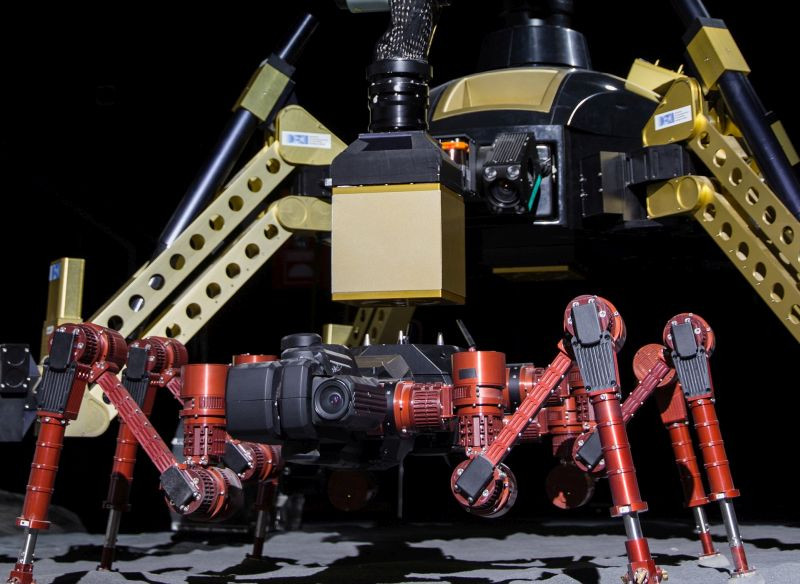
\includegraphics[width=0.8\linewidth]{pictures/RIMRES-final-14}\\
  %\vspace{-2ex}
  \caption[A sample image]
          {A sample image. This is a longer caption than that used for the index.}
  \label{fig:RIMRES-final-14}
  %\vspace{-3ex}
\end{figure}

\begin{figure}%[b]
\vspace{-2ex}
	\centering
    %% setup sizes
    \setlength{\subfigureWidth}{0.32\textwidth}
    \setlength{\graphicsHeight}{33mm}
    %% kill hyper-link highlighting
    \hypersetup{hidelinks=true}%
    %% the figures
	\begin{subfigure}[t]{\subfigureWidth}
        \centering
		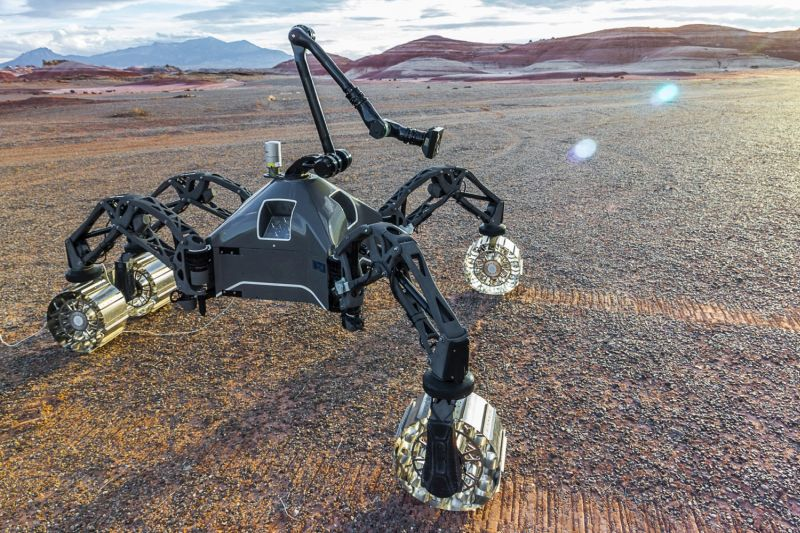
\includegraphics[height=\graphicsHeight]{pictures/SherpaTT_QuasiTripod}
		\subcaption{Quasi tripod pose}
		\label{fig:SherpaTT_QuasiTripod}
	\end{subfigure}\hfill
	\begin{subfigure}[t]{\subfigureWidth}
        \centering
		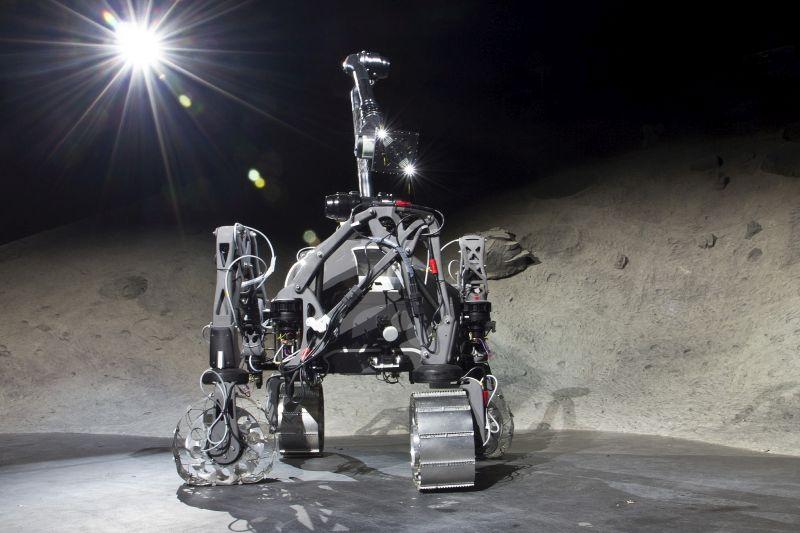
\includegraphics[height=\graphicsHeight]{pictures/SherpaTT_Stow}
		\subcaption{Compact stow pose of legs}
		\label{fig:SherpaTT_Stow}
	\end{subfigure}\hfill
    \begin{subfigure}[t]{\subfigureWidth}
        \centering
		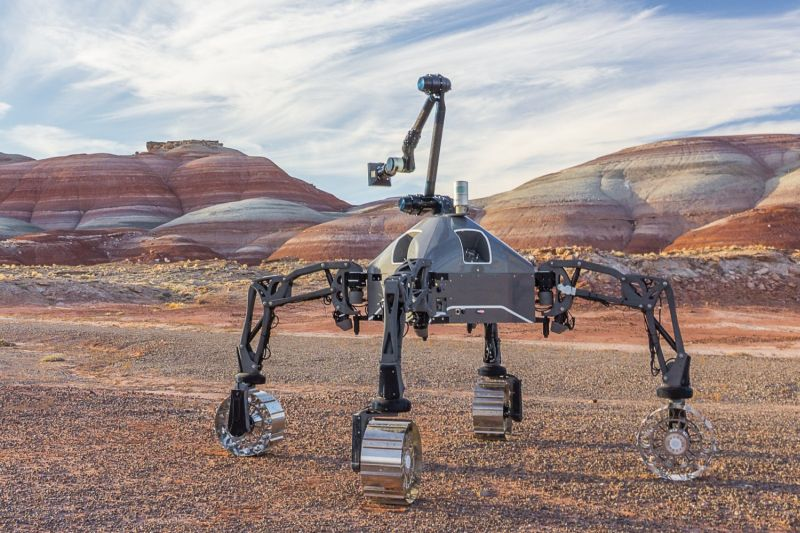
\includegraphics[height=\graphicsHeight]{pictures/SherpaTT_HighPose}
		\subcaption{High body pose in CrossStance}
		\label{fig:SherpaTT_HighPose}
	\end{subfigure}\\[0.8ex]
%% 2nd row
    \begin{subfigure}[t]{\subfigureWidth}
        \centering
		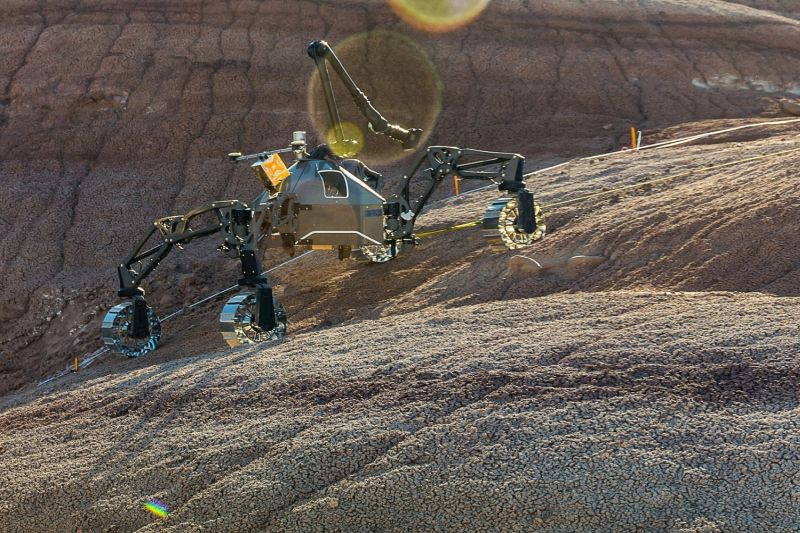
\includegraphics[height=\graphicsHeight]{pictures/SherpaTT_RPA_Utah}
		\subcaption{Body roll-pitch control in sloping natural terrain}
		\label{fig:SherpaTT_RPA_Utah}
	\end{subfigure}\hfill
	\begin{subfigure}[t]{\subfigureWidth}
        \centering
		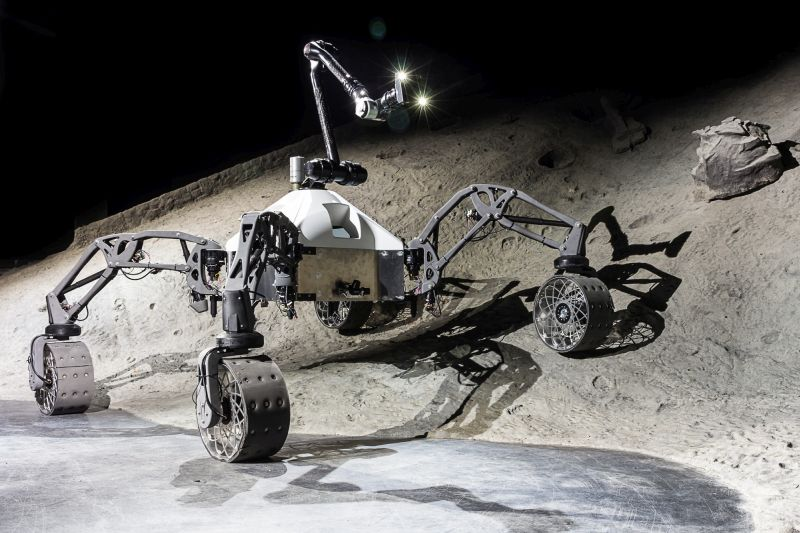
\includegraphics[height=\graphicsHeight]{pictures/SherpaTT_RPA_Crater}
		\subcaption{Body roll-pitch control in artificial crater}
		\label{fig:SherpaTT_RPA_Crater}
	\end{subfigure}\hfill
    \begin{subfigure}[t]{\subfigureWidth}
        \centering
		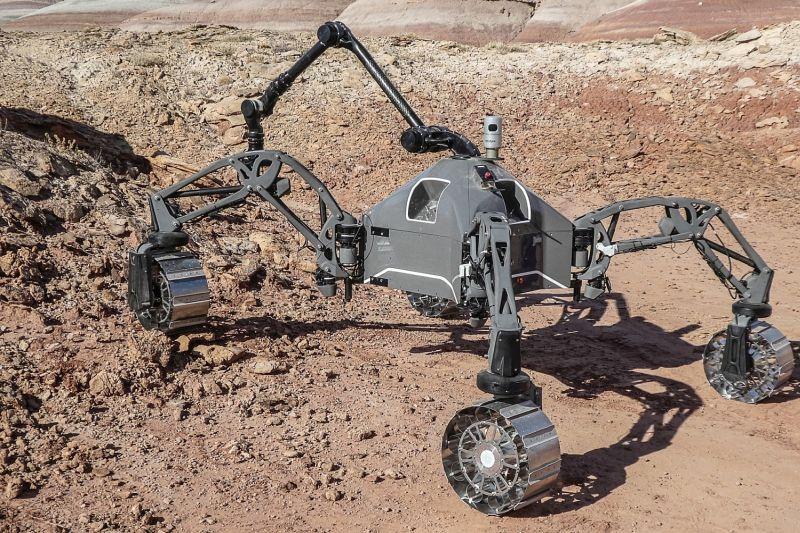
\includegraphics[height=\graphicsHeight]{pictures/SherpaTT_SamplingUtah}
		\subcaption{Approaching a sampling spot in natural terrain}
		\label{fig:SherpaTT_SamplingUtah}
	\end{subfigure}
	\caption{Example of a figure with subfigures}
	\label{fig:SherpaTT}
\vspace{-2ex}
\end{figure}


\begin{table}%[h]
%\vspace{-2ex}
  %\centering
  \hypersetup{hidelinks=true}
  %
  \caption[Exemplary table]{Exemplary table.
  \dissExtraCaption{With an example of an extra caption. Should be used with optional caption.}
  }
  \label{tab:Design:ComparisonSherpaSherpaTT}
  \begin{footnotesize}
      \begin{tabular}{l| rrr r ll r rr}
        \toprule
         \rowcolor{tableheadingcolor}
        System  & Leg length & Mass    & Mass & \ac{DoF}         & vert. & horz. & min stow  & \multicolumn{2}{c}{compactness}\\
        \rowcolor{tableheadingcolor}
                & zero pose &  (leg)  & total  & (leg)   & stroke &  stroke &volume    & footprint & volume \\
        \midrule
        \cellcolor{tablesubheadingcolor}Sherpa      & 976\unitmm & 25\unitkg & 160\unitkg &6          & 900\unitmm
%        \color{captionTextColor}{$^{\ast}$}
        & 260\unitmm
%        \color{captionTextColor}{$^{\ast\ast}$}
        &  2.24\unitcubmeter & 0.40 & 0.64\\
        \cellcolor{tablesubheadingcolor}SherpaTT\hspace{-1mm}    & 977\unitmm & 26\unitkg & \massSherpaTT &5          & 775\unitmm & 485\unitmm & 1.67\unitcubmeter & 0.79 & 0.72\\
        \bottomrule
      \end{tabular}
  \end{footnotesize}
\end{table}





\section{Structure of Thesis}
The structure of this thesis is illustrated in \refFig{fig:structure_diagram}. \todo{if you do not want to use citations, check \swCmd{styles/structureGraphFunctions.tex} with the example of an alternative \swCmd{\textbackslash drawChapterBox} command}
From the publications forming this cumulative thesis, those related to each chapter are provided in the respective box.
Further publications of the author are cited at the appropriate places in each paragraph.



\begin{figure}%[htb]
    \begin{center}
        %%%%%%%%%%%%%%%%%%%%%%%%%%%%%%%%%%%%%%%%
%%% structural graph of thesis document
%%%%%%%%%%%%%%%%%%%%%%%%%%%%%%%%%%%%%%%%


%% helper for minipages
%%  \begin{minipage}[outerPos][height][innerPos]{width}
%%	     Beispieltext
%%  \end{minipage}
%% outerPos (optional; c,t,b): where the minipage is on the page (center, top, bottom)
%% height (optional): height o minipage, regardless of contents
%% innerPos (optional; c,t,b): where the content is (center, top, bottom)

% set some dimension variables for minipages
\newlength{\structureGraphHeight}
\setlength{\structureGraphHeight}{100mm}

\newlength{\chapterboxWith}
\setlength{\chapterboxWith}{0.45\linewidth}

\newlength{\chapterboxHeight}
\setlength{\chapterboxHeight}{21mm}





%%% the actual graph







%%%%%%%%%%%%%%%%%%%%%%%%%%%%%%%%%%%%%%%%%%%%%%%%%%%%%%%%%%%%%%%%%%%%%%%%%%%%%%%%%%%%%%%%%%%%%%%%%%%%%%%%%%%%%
%% this is the actual structure plot
%% settings are in   thesis_colors.sty   and   styles/structrueGraphFunctions.tex
%%



%\begin{tcolorbox}[code={\pgfkeysalsofrom{\outerboxoptions}},
%                  title=Thesis: \newline\qq{\myWorkingTitle}]
    %external raster
    \begin{tcbraster}[ code={\pgfkeysalsofrom{\outerrasteroptions}} ]
            %ROW 1                                                        % |-- SINGLE-box-Options
            \partbox{Intro}{}{                                            % v
                \begin{tcboxedraster}[ code={\pgfkeysalsofrom{\innerrastersinglecoloptions}} ]{blankest}
                        \rule{0.25\linewidth}{0pt}% remove for dual
                        \drawChapterbox{sec:introduction}{\introCites}%
                        %\rule{0.2\linewidth}{0pt}%
                \end{tcboxedraster}
            }
            % ROW2
            \partbox{Foundations}{}{
                \begin{tcboxedraster}[ code={\pgfkeysalsofrom{\innerrasterdualcoloptions}} ]{blankest} 
                        \drawChapterboxSota{sec:sota}{ \sotaCites }%
                        \drawChapterbox{sec:ReqirementsConditions}{ ~ }%
                \end{tcboxedraster}
            }
            % ROW3                                                       % |-- DUAL-box-Options
            \partbox{Design}{}{                                          % v
                \begin{tcboxedraster}[ code={\pgfkeysalsofrom{\innerrasterdualcoloptions}} ]{blankest} %<- no drawn box or white space around inner boxes
                        \drawChapterbox{sec:RobotDesign}{ \designCites }%
                        \drawChapterbox{sec:control}{ \controlCites }%
                \end{tcboxedraster}
            }
            %ROW 4
            \partbox{~~Experi-}{mentation}{
                \begin{tcboxedraster}[ code={\pgfkeysalsofrom{\innerrastersinglecoloptions}} ]{blankest}
                        \rule{0.25\linewidth}{0pt}%
                        \drawChapterbox{sec:Experiments}{ \expCites }%
                        %\rule{0.2\linewidth}{0pt}%
                \end{tcboxedraster}
            }
            %ROW 5
            \partbox{Conclusion}{}{
                \begin{tcboxedraster}[ code={\pgfkeysalsofrom{\innerrastersinglecoloptions}} ]{blankest}
                        \rule{0.25\linewidth}{0pt}%
                        \drawChapterbox{sec:ConclusionOutlook}{ \conclusionCites }%
                        %\rule{0.2\linewidth}{0pt}%
                \end{tcboxedraster}
           }
            %ROW 6
            \partbox{Appendix}{}{
                \begin{tcboxedraster}[ code={\pgfkeysalsofrom{\innerrastertriplecoloptions}} ]{blankest}
                        %\rule{0.25\linewidth}{0pt}%
                        \drawAppendixbox{sec:Appendix:AdditionalMaterial}{ ~ }%
                        \drawAppendixbox{sec:Appendix:MoreStuff}{ ~ }%
                        \drawAppendixbox{sec:Appendix:Enough}{ ~ }%
                        %\rule{0.2\linewidth}{0pt}%
                \end{tcboxedraster}
            }
    \end{tcbraster}
%\end{tcolorbox}	














    \end{center}
    \vspace{-1ex}
    \caption{Structure of this thesis and related publications per chapter.}
    \label{fig:structure_diagram}
    %\vspace{-1.8ex}
\end{figure}


\section{Bibliography Remarks}
\label{sec:intro:BibRemarks}
\todo{run the \swCmd{make\_bib.bat} file or the command lines within to generate the bibliography}
To better distinguish between the author's own publications and citations from literature, different citation marks are applied:
\begin{compactitem}
  \item Citations from the author's own publications are plain numbered, \eg~\citeown{myPubA}, \citeown{myPubB}. 
  \item Citations from literature are using the author-year format, \eg~\citesota{Wilcox2012}.
\end{compactitem}




%%%%%%%%%%%%%%%%%%%%%%%%%%%%%%%%%%%%%%%%%%%%%%%%%%%%%%%




%%%%%%%%%%%%%%%%%%%%%%%%%%%%%%%%%%%%%%%%%%%%%%%%%%%%%%%
%#%\chapter{State of the Art}
%#%\label{sec:sota}
%\acresetall                 %% reset all acronym abbreviations and write first appearance long
%\acused{CAD}
\acused{DoF}
\acused{EEPROM}
\acused{FPGA}
\acused{GPS}
\acused{HD}
\acused{LED} %%define ackronyms that are "common sense"
%#%
\shinyChapterQuote{A shiny quote for the start?}
       {If you like to.}

This chapter gives a brief overview on the \SOTA of the main topics of this thesis.
\todo[inline]{adapt to your own thesis!}

%\chapterSupportedBy{\sotaCites}
%\sotaCites
%\todo{check long list vs. short list macros!}
\chapterSupportedBy{\sotaCitesLong}




\section{A Section of this Chapter}
\label{sec:sota:ASection}
%\input{sections/.tex}

\section{Another Section of this Chapter}
\label{sec:sota:AnotherSection}
%\input{sections/.tex}

%%%%%%%%%%%%%%%%%%%%%%%%%%%%%%%%%%%%%%%%%%%%%%%%%%%%%%%

%%%%%%%%%%%%%%%%%%%%%%%%%%%%%%%%%%%%%%%%%%%%%%%%%%%%%%%
\chapter{Introduction}
%\shinyChapterQuote{}
\label{sec:Introduction}
\todo[inline]{\textbf{TODO:} Write chapter introduction.}

\section{Background}
\label{sec:Introduction:Background}
The rover SherpaTT has been deployed in several field experiments where it was put under test within natural and unstructured Mars analogue terrain with respect to general morphology and geology. The rover displayed the ability to cope with natural terrain and to fulffill the task of being an exploration and sampling rover. Currently, the rover is prepared for further autonomous long distance traverses in terrain akin to the Martian environment. However, it features a fueled power generator which cannot be employed in Martian or Lunar missions and limits the system's autonomous mission lifetime to the discharge rate of its two LiPo batteries.

As the rover is meant to approach a higher technology readiness level, further development is required on its electrical power subsystem if it is to operate in long term missions. This thesis will explore solar array configurations with respect to constraints imposed by the Martian environment so that future versions of the rover may be designed to navigate the topography of this planetary surface. The constraints imposed from the active suspension system with flexible footprints and varying heights of structural parts of the legs are considered in the design phase.

Mars mission scenarios will be explored in order to propose solar array requirements and impose power storage and consumption constraints based on sol-by-sol analysis of solar insolation as a function of geographic latitude, areocentric longitude, atmospheric opacity, dust deposition, and sun angle of incident on the solar array. The mission scenario will put particular emphasis on including topograpy best tackled by the rover's wheeled leg design, such as climbing up mountains and volcanoes or going down valleys and craters. Sites with high geological and exobiological science potential typically require navigating complicated terrains which offer an opportunity for further power budget analysis that take into account solar insolation on an inclined surface.

\todo[inline]{TODO: Reference DFKI literature regarding SherpaTT, specifically the field trials.}

\todo[inline]{TODO: Expand the introduction to introduce the structure of the thesis.}


%A Lunar mission scenario will also be investigated with particular interest on access to permanently shadowed areas in the southern pole. The mission scenarios will put particular emphasis on including topograpy best tackled by the rover's wheeled leg design, such as climbing up mountains and volcanoes or going down valleys and craters. Sites with high geological and exobiological science potential typically require navigating complicated terrains which offer an opportunity for further power budget analysis that take into account solar irradiance on slopes.


\section{Scope and Contributions}
\label{sec:Introduction:ScopeAndContributions}
This thesis builds upon the areas of interest elaborated in previous work. Notably, it acknowledges that the rover is intended to be part of a heterogeneous modular \ac{MRS} and that a wealth of data has been collected over the course of multiple field test campaigns. Radical system changes are avoided and design constraints are driven by the collected performance measurements. Design changes made to accomodate the proposed \ac{PV} system will be mindful of mission objectives inherent with scenarios such as crater exploration and operating within a sample return logistics chain.

The main contribution of this thesis is the design of \acp{SA} for the rover at two Mars mission sites. These sites are selected so that the distinct requirements between different solar radiation environments may be appreciated. Re-usability of the implemented solutions is taken into account throughout the entire development of the thesis. As such, formulas and calculations pertaining to solar radiation as well as power and energy predictions have been packged into a thoroughly documented general purpose R library. Furthermore, a rudimentary power calculation plugin is developed as a prototype for the MARS real-time robotic simulation and visualisation tool. This plugin offers insights on how the Blender/Phobos robot modeling software suite may be extended to support modeling solar panels as robot sensors.

Further contributions pertain to formalizing requirements and constraints that need to be considered for future solar powered iterations of the rover towards reaching higher \acp{TRL}. Beyond the Martian environment, the proposed solution serves as a template to integrating solar powered systems for other celestial bodies such as in terrestial and lunar mission scenarios.

Finally, this thesis provides an alternative use case for the rover's active suspension system. Thus far, explored opportunities granted by such a system have been restricted to analyzing its benefits with respect to traversing challenging topographies. Introducing how such a system can be leveraged for other aspects of mission planning broadens the field of research.


\section{Structure of Thesis}
\label{sec:Introduction:StructureOfThesis}
The thesis is structured in five chapters. The foundation of the thesis are presented in the two chapters following the introduction. Power subsystems of past, ongoing, and planned missions are briefly introduced in Chapter \ref{sec:StateOfTheArt}. The \ac{SOA} of solar and battery cell technologies built on top of mission heritage are then summarized. Chapter \ref{sec:MarsSolarEnergy} rigorously explores the Martian solar radiation environment from which two mission sites are selected. These serves as the primary driver in defining worst case scenarios that will impose environmental design constraints.

The design of the proposed \ac{PV} power system is described in Chapter \ref{sec:PowerSystemDesign}. Reference Sols and their power budgets are formalized in order to fine tune feasable requirements and design drivers. Two distinct \ac{SA} designs are presented for each mission site and a brief simulation prototype is introduced. The thesis is concluded in Chapter \ref{sec:ConclusionAndOutlook} which also provides an outlook for future research and developments.

Additional material is provided in Appendices. Verification of the mars solar insolation R package developed for this thesis is presented in Appendix \ref{sec:Appendix:InsolationCalculationVerification}. The solar energy predictions calculated by the R package was also validate against \ac{MER} ground truth data. An attempt to reduce the observed divergences is elaborated in Appendix \ref{sec:Appendix:EnergyErrorMargin}. Finally, background information regarding optimal \ac{SA} inclination and orientation angles are found in Appendix \ref{sec:Appendix:OptimalAngles}.


\section{Summary and Conclusion}
\label{sec:Introduction:SummaryAndConclusion}
\todo[inline]{\textbf{TODO:} Write summary and conclusion for this chapter.}

%%%%%%%%%%%%%%%%%%%%%%%%%%%%%%%%%%%%%%%%%%%%%%%%%%%%%%%

%%%%%%%%%%%%%%%%%%%%%%%%%%%%%%%%%%%%%%%%%%%%%%%%%%%%%%%
\chapter{State of the Art}
%\shinyChapterQuote{}
\label{sec:StateOfTheArt}
This chapter briefly explores the state of art in space grade solar and battery cell technologies. \refSec{sec:StateOfTheArt:PastAndOngoingMissions} presents a historical overview of past and ongoing missions. The state of practice is briefly touched upon in \refSec{sec:StateOfTheArt:PlannedMissions} as a segue to the chapter's conclusion with the state of art in \refSec{sec:StateOfTheArt:PhotovoltaicsAndEnergyStorage}.

\section{Past and Ongoing Missions}
\label{sec:StateOfTheArt:PastAndOngoingMissions}
% Image source:
% MER
% https://mars.nasa.gov/mer/

% All others:
% https://science.nasa.gov/toolkits/spacecraft-icons
The scope of this section is restricted to successful missions. At the time of writing this thesis, the \ac{NASA} remains the only organization to successfully land and operate a spacecraft on the Martian surface. Two types of missions are explored: landers and rovers. Descriptions of these missions are restricted to power generation and storage characteristics.

\subsection{Landers}
\label{sec:StateOfTheArt:PastAndOngoingMissions:Landers}

Successful landers are shown in Figure \ref{fig:past-mission-landers}. The Viking Program involved two space probes: Viking 1 and Viking 2. Each were composed of an orbiter and a lander, identified as \ac{VL1} and \ac{VL2} shown Figure \ref{fig:sub:past-mission-lander-viking}. The Phoenix lander, shown in Figure \ref{fig:sub:past-mission-lander-phoenix} was part of the Mars Scout Program. The ongoing InSight mission lander is part of the Discovery Program and is shown in Figure \ref{fig:sub:past-mission-lander-insight}.

\vspace{0.5cm}

\begin{figure}[h]
\captionsetup[subfigure]{justification=centering}
\vspace{-2ex}
	\centering
    %% setup sizes
    \setlength{\subfigureWidth}{0.48\textwidth}
    \setlength{\graphicsHeight}{31mm}
    %% kill hyper-link highlighting
    \hypersetup{hidelinks=true}%
    %% the figures
	\begin{subfigure}[t]{\subfigureWidth}
        \centering
		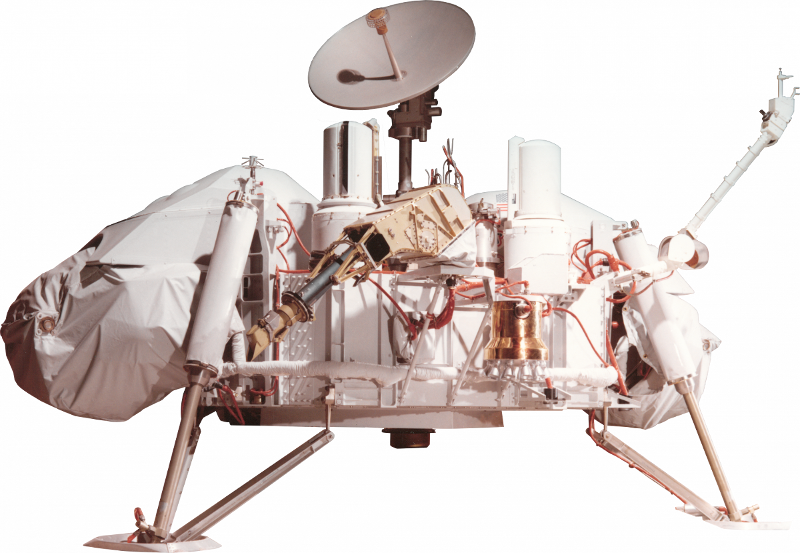
\includegraphics[height=\graphicsHeight]{sections/state-of-the-art/past-missions/images/lander-viking.png}
		\subcaption{Viking}
		\label{fig:sub:past-mission-lander-viking}
	\end{subfigure}\\[0.8ex]
%% 2nd row
	\begin{subfigure}[t]{\subfigureWidth}
        \centering
		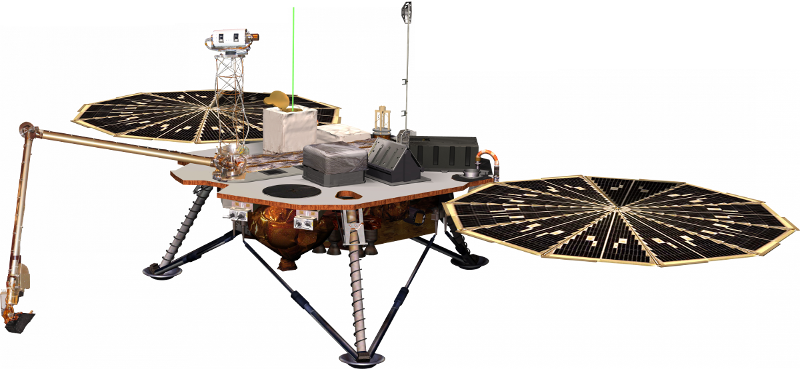
\includegraphics[height=\graphicsHeight]{sections/state-of-the-art/past-missions/images/lander-phoenix.png}
        \subcaption{Phoenix}
		\label{fig:sub:past-mission-lander-phoenix}
	\end{subfigure}\hspace*{0.5cm}
    \begin{subfigure}[t]{\subfigureWidth}
        \centering
		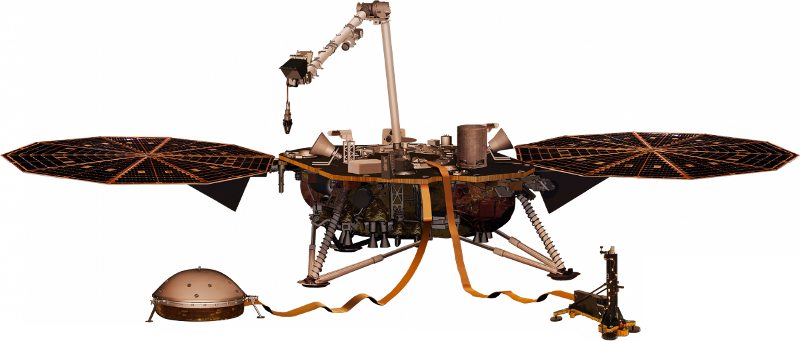
\includegraphics[height=\graphicsHeight]{sections/state-of-the-art/past-missions/images/lander-insight.png}
		\subcaption{InSight}
		\label{fig:sub:past-mission-lander-insight}
	\end{subfigure}
    \caption[Past and ongoing lander missions]
            {Past and ongoing lander missions.}
	\label{fig:past-mission-landers}
\vspace{-2ex}
\end{figure}

% Alternative layout of lander figures. All 3 subfigures in a single line.
\begin{comment}
\begin{figure}[h]
\captionsetup[subfigure]{justification=centering}
\vspace{-2ex}
	\centering
    %% setup sizes
    \setlength{\subfigureWidth}{0.32\textwidth}
    \setlength{\graphicsHeight}{21mm}
    %% kill hyper-link highlighting
    \hypersetup{hidelinks=true}%
    %% the figures
	\begin{subfigure}[t]{\subfigureWidth}
        \centering
		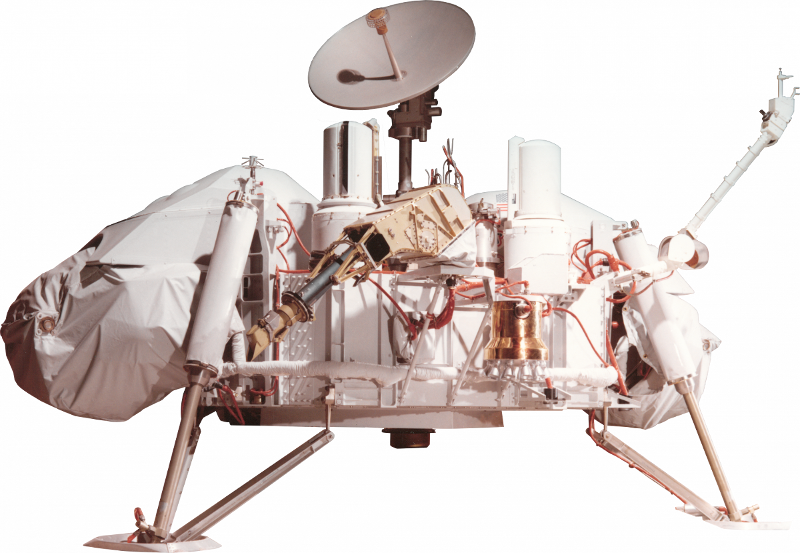
\includegraphics[height=\graphicsHeight]{sections/state-of-the-art/past-missions/images/lander-viking.png}
		\subcaption{Viking Lander}
		\label{fig:sub:past-mission-lander-viking}
	\end{subfigure}\hfill
	\begin{subfigure}[t]{\subfigureWidth}
        \centering
		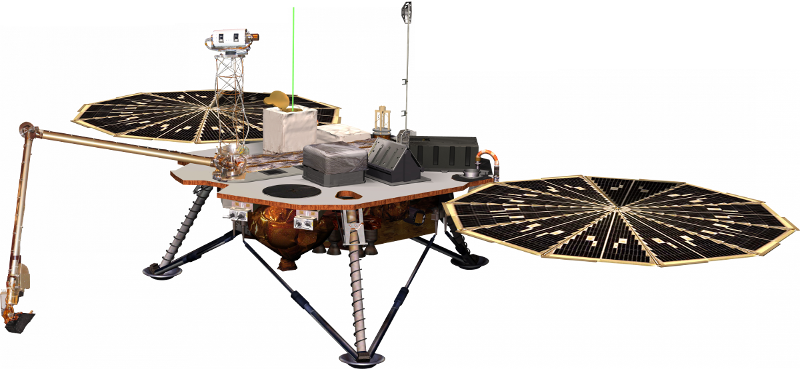
\includegraphics[height=\graphicsHeight]{sections/state-of-the-art/past-missions/images/lander-phoenix.png}
		\subcaption{Phoenix Lander}
		\label{fig:sub:past-mission-lander-phoenix}
	\end{subfigure}\hfill
    \begin{subfigure}[t]{\subfigureWidth}
        \centering
		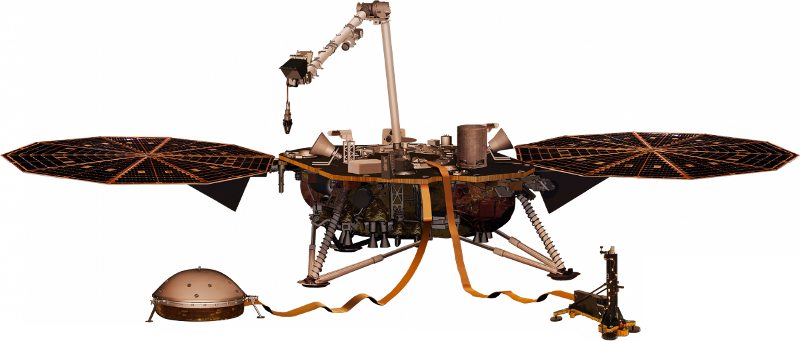
\includegraphics[height=\graphicsHeight]{sections/state-of-the-art/past-missions/images/lander-insight.png}
		\subcaption{InSight Lander}
		\label{fig:sub:past-mission-lander-insight}
	\end{subfigure}
	\caption[Past and ongoing lander missions]
            {Past and ongoing lander missions.}
	\label{fig:past-mission-landers}
\vspace{-2ex}
\end{figure}
\end{comment}

\subsubsection{Viking}

A single Viking Lander was powered by two \ac{RTG} units. Converting heat from decaying plutonium-236 resulted in a continuous nominal electrical power output of \SI{70}{\watt} at \SI{4.4}{\volt}. Four \SI{30}{\volt} nominal, 42-cell \ac{NiCd} batteries were mounted in pairs and charged by the \ac{RTG} units. The battery cells were \SI{8}{\ampere\hour} at \ac{EOL}. Recharge rates depended on available \ac{RTG} energy and varied from C/40 to C/6. Descrease in charge efficieny tied to temperature increase imposed a thermal constraint in which charging did not occur if the battery temperature was greater than \SI{21}{\degree} in order to prevent excessive battery temperatures during charging. Further power subsytem design details can be found in \citepower{Holmburg1980}.

\subsubsection{Phoenix}

The Phoenix Lander generated power from its two ATK ``UltraFlex'' \acp{SA} which covered a total surface area of \SI{4.2}{\meter\squared}. The \acp{SA} provided approximately \SI{22}{\watt/\kilo\gram} under Mars conditions \citepower{Badescu2009} \citeother{Linne2012}. Its round fan-fold design unfoled into two separate circular decagon panels. Two rechargeable \ac{Li-ion} \ac{NCO}-cell batteries were manufactured by Yardney and had a nameplate capacity of \SI{25}{\ampere\hour}. The battery cells were arranged in an 8s2p configuration, capacity voltage range was 50‒62 \si{\volt}, operating voltage range 24‒\SI{32.8}{\volt}, mass \SI{17.8}{\kilo\gram}, specific energy \SI{105}{\watt\hour/\kilo\gram}, and the operating temperature was from \SI{-20}{\celsius} to +\SI{30}{\celsius} \citepower{NASAEnergyStorage2017}.

\subsubsection{InSight}

The InSight Lander is based on heritage from the Phoenix mission and as such shares similar characteristics. It generates power from two \acp{SA} each measuring \SI{2.2}{\meter} in diameter. The \acp{SA} are  ATK ``UltraFlex'' ZTJ triple-junction solar cells made of \ac{InGaP}/\ac{InGaAs}/\ac{Ge}. The \ac{NCA}-cells rechargeable batteries were manufactured by Yardney and based on Phoenix's NCP‒25‒1 cell design. The two 8-cell in parallel (8s2p), \SI{28}{\volt}, \SI{30}{\ampere\hour} batteries can operate down to \SI{-35}{\celsius} \citepower{EaglePitcher}. As listed in \citepower{Smart2015}, the battery performance requirements for InSight are:

\begin{itemize}
  \item The battery shall support 709 sols of surface operations over a temperature range of \SI{-30}{\celsius} to +\SI{35}{\celsius}.
  \item Each 8-cell battery shall be able to support a \SI{5}{\ampere} charge rate over the entire allowable flight temperature range of \SI{-30}{\celsius} to +\SI{35}{\celsius}.
  \item Each 8-cell battery shall provide at least \SI{25}{\ampere\hour} at \SI{-25}{\celsius} \ac{BOL} over the voltage range of \SI{24}{\volt} to \SI{32.8}{\volt} using a C/5 rate (\SI{5}{\ampere}).
\end{itemize}

\clearpage
\subsection{Rovers}
\label{sec:StateOfTheArt:PastAndOngoingMissions:Rovers}

Successful rovers are shown in Figure \ref{fig:past-mission-rovers}. The Sojourner rover was the first rover to operate on the Martian surface and is shown in Figure \ref{fig:sub:past-mission-rover-sojourner}. The \ac{MER} mission consisted of twin rovers  Spirit and Opportunity shown in Figure \ref{fig:sub:past-mission-rovers-mer}. The ongoing \ac{MSL} Curiosity mission is part of the \ac{MEP} and shown in Figure \ref{fig:sub:past-mission-rovers-msl}.

\begin{figure}[h]
\captionsetup[subfigure]{justification=centering}
\vspace{-2ex}
	\centering
    %% setup sizes
    \setlength{\subfigureWidth}{0.45\textwidth}
    \setlength{\graphicsHeight}{35mm}
    %% kill hyper-link highlighting
    \hypersetup{hidelinks=true}%
    %% the figures
	\begin{subfigure}[t]{\subfigureWidth}
        \centering
        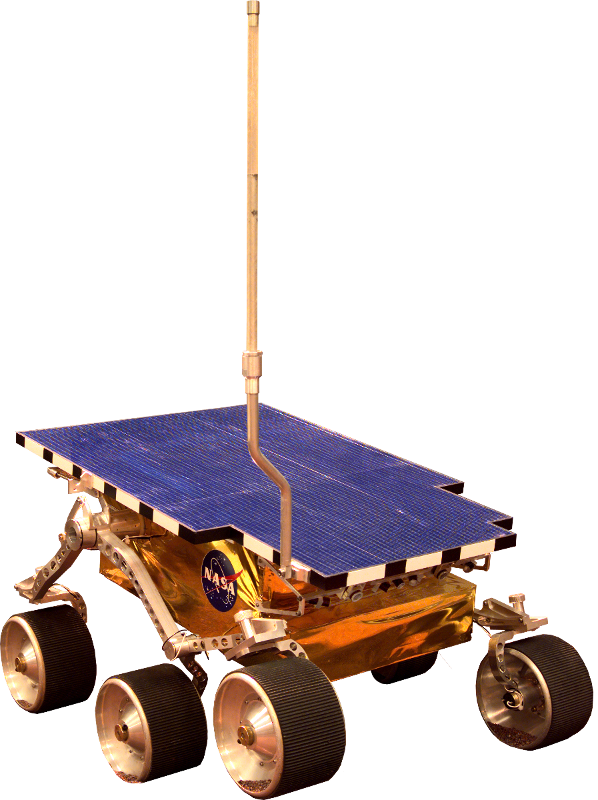
\includegraphics[height=\graphicsHeight]{sections/state-of-the-art/past-missions/images/rover-sojourner.png}
        \subcaption{Sojourner}
        \label{fig:sub:past-mission-rover-sojourner}
	\end{subfigure}\\[0.8ex]
%% 2nd row
	\begin{subfigure}[t]{\subfigureWidth}
        \centering
		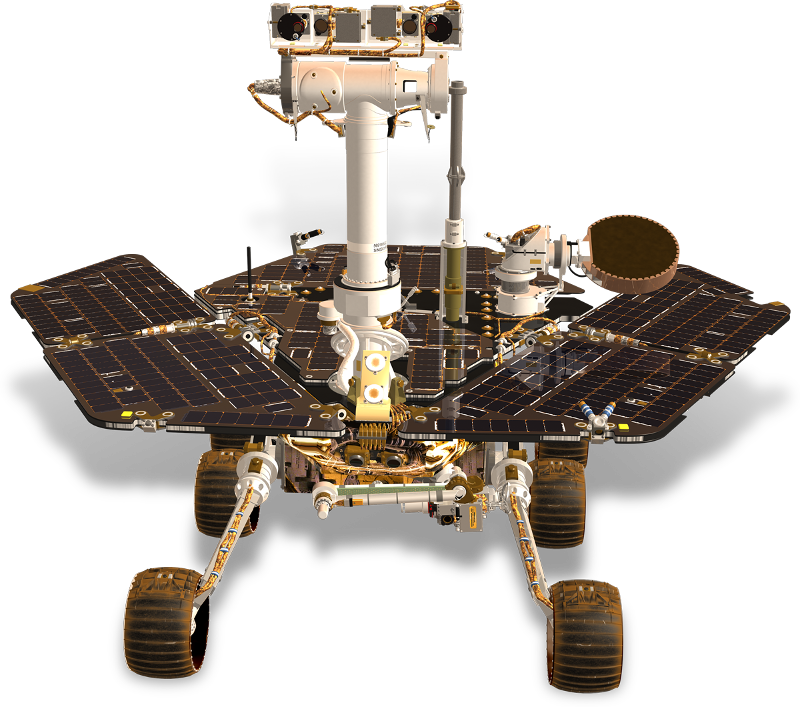
\includegraphics[height=\graphicsHeight]{sections/state-of-the-art/past-missions/images/rover-mer.png}
		\subcaption{MER Opportunity and Spirit}
		\label{fig:sub:past-mission-rovers-mer}
	\end{subfigure}\hspace*{0.5cm}
    \begin{subfigure}[t]{\subfigureWidth}
        \centering
		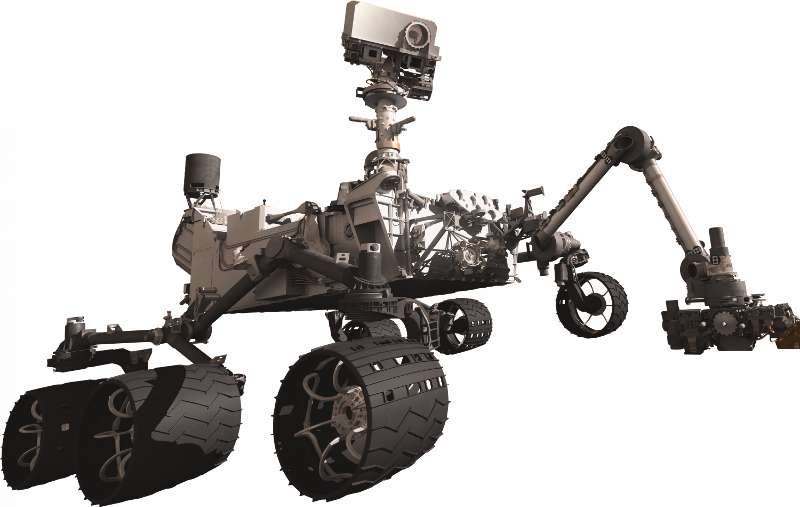
\includegraphics[height=\graphicsHeight]{sections/state-of-the-art/past-missions/images/rover-msl.png}
		\subcaption{MSL Curiosity}
		\label{fig:sub:past-mission-rovers-msl}
	\end{subfigure}
    \caption[Past and ongoing rover missions]
            {Past and ongoing rover missions.}
	\label{fig:past-mission-rovers}
\vspace{-2ex}
\end{figure}

\begin{comment}

\vspace{0.5cm}

\begin{figure}[h]
\captionsetup[subfigure]{justification=centering}
\vspace{-2ex}
	\centering
    %% setup sizes
    \setlength{\subfigureWidth}{0.32\textwidth}
    \setlength{\graphicsHeight}{30mm}
    %% kill hyper-link highlighting
    \hypersetup{hidelinks=true}%
    %% the figures
	\begin{subfigure}[t]{\subfigureWidth}
        \centering
		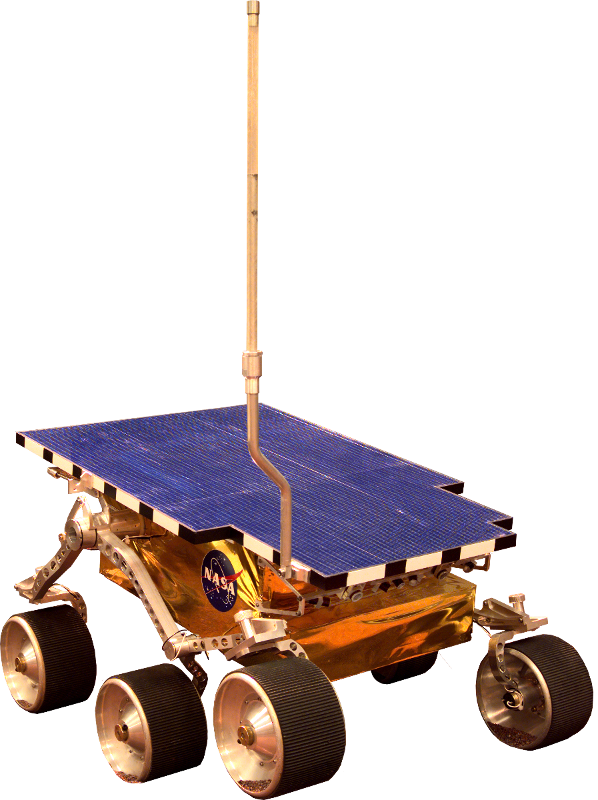
\includegraphics[height=\graphicsHeight]{sections/state-of-the-art/past-missions/images/rover-sojourner.png}
		\subcaption{Sojourner}
		\label{fig:sub:past-mission-rover-sojourner}
	\end{subfigure}\hfill
	\begin{subfigure}[t]{\subfigureWidth}
        \centering
		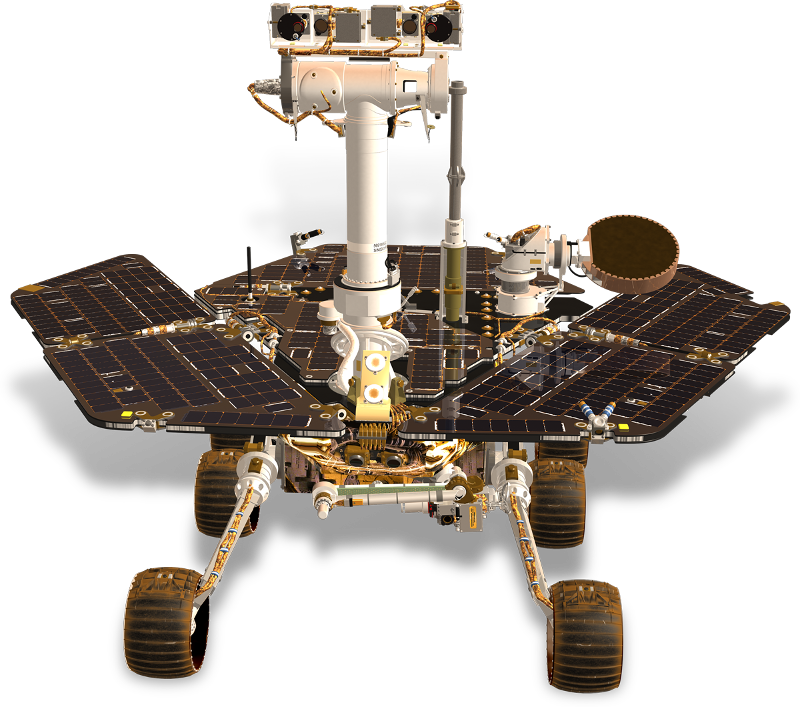
\includegraphics[height=\graphicsHeight]{sections/state-of-the-art/past-missions/images/rover-mer.png}
		\subcaption{MER Opportunity and Spirit}
		\label{fig:sub:past-mission-rovers-mer}
	\end{subfigure}\hfill
    \begin{subfigure}[t]{\subfigureWidth}
        \centering
		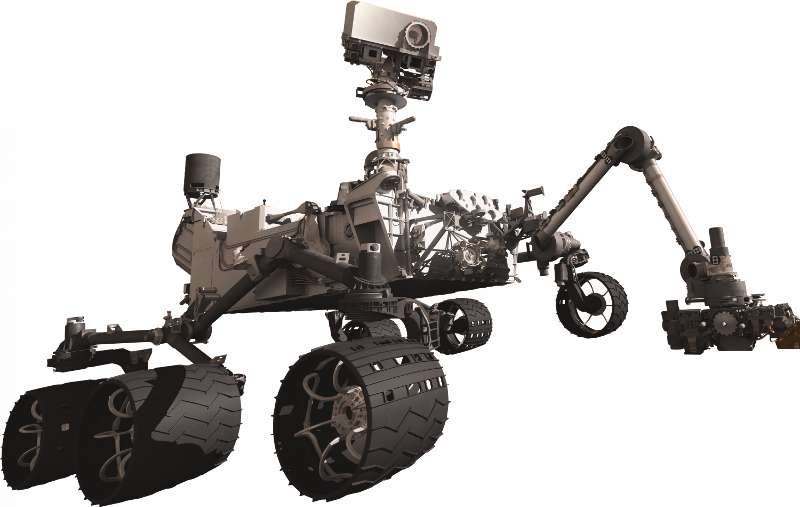
\includegraphics[height=\graphicsHeight]{sections/state-of-the-art/past-missions/images/rover-msl.png}
		\subcaption{MSL Curiosity}
		\label{fig:sub:past-mission-rovers-msl}
	\end{subfigure}
	\caption[Past and ongoing rover missions]
            {Past and ongoing rover missions.}
	\label{fig:past-mission-rovers}
\vspace{-2ex}
\end{figure}
\end{comment}

\subsubsection{Sojourner}
The Sojourner microrover was powered by a 0.22\si{\meter\squared}, $\SI{2}{\centi\meter}\times\SI{4}{\centi\meter}$, 5.5 mil thick \ac{GaAs}/\ac{Ge} solar panel. it provided around \SI{16.5}{\watt} of power at solar noon and the operating temperature was from \SI{-140}{\celsius} to +\SI{110}{\celsius}. Each of its three batteries were configured as 3 \ac{Li-SOCL2} D-size cells arranged in series and provided up to \SI{150}{\watt\hour}. The battery cell capacity was \SI{12}{\ampere\hour} at +\SI{25}{\celsius} and \SI{8}{\ampere\hour} at \SI{-20}{\celsius}. Operating voltage was 8‒11 \si{\volt} and mass was 1.24 \si{\kilo\gram}. The rover's power system allowed it to draw of up \SI{30}{\watt} of peak power with a peak solar panel power output of \SI{16}{\watt}. The rover's nominal propulsion power requirement is \SI{10}{\watt}. Further details on Sojourner's power subsystem can be found in \citepower{SojournerDescription} and \citepower{SojournerPowerSubsystem}.

\subsubsection{Opportunity and Spirit}
The twin rovers generated power from their triplejunction \ac{GaInP}/\ac{GaAs}/\ac{Ge} \acp{SA} with a solar cell coverage area of \SI{1.3}{\square\meter}. The \acp{SA} could generate almost \SI{900}{\watt\hour} of energy at \ac{BOL} on a clear day in absence of dust deposition \citepower{Badescu2009}. The rovers's propulsion power draw was approximately \SI{100}{\watt}. Two rechargeable \ac{Li-ion} NCP-8-1 \ac{NCO}-cell batteries weighing \SI{7.15}{\kilo\gram} were manufactured by Yardney and provided support to the \ac{SA} as well as enabled nighttime experiments \citepower{Badescu2009}. Each battery was configured in 8-cell \SI{10}{\ampere\hour} strings connected in parallel (8s2p). The nameplate capacity was \SI{8}{\ampere\hour} and the \ac{DOD} was designed to typically be 40‒50 \si{\percent} per Sol \citepower{Gulbinska2014}. Capacity voltage range was 16‒20 \si{\volt}, operating voltage range 24‒32.8 \si{\volt}, specific energy \SI{90}{\watt\hour/\kilo\gram}, and the operating temperature was from \SI{-20}{\celsius} to +\SI{30}{\celsius} \citepower{NASAEnergyStorage2017}. The rovers were heated by eight \acp{RHU}, each of which continuously generated \SI{1}{\watt} of thermal energy. The following are notable battery operational requirements taken from \citepower{Gulbinska2014}:

\begin{itemize}
  \item Maintaining the operating voltage of 24‒36 \si{\volt}.
  \item Providing sufficient energ for surface operations ($\geq$ \SI{283}{\watt\hour} per Sol at \SI{0}{\celsius}).
  \item Delivering sufficiently long cycle life ($\geq$ 270 cycles at \SI{50}{\percent} \ac{DOD} and/or 90 Sols operation).
  \item The battery should successfully charge and discharge between -20 and +\SI{30}{\celsius} throughout the length of the entire mission.
\end{itemize}

\subsubsection{Curiosity}
The Curiosity rover uses the \ac{MMRTG} power system. Is is designed to initially provide around \SI{2000}{\watt} of thermal power and \SI{110}{\watt} of electrical power in a deep space environment \citepower{MMRTG}. The electrical output is used to charge its two Yardney \ac{Li-ion} NCP-42-1 \ac{NCO}-cell batteries, which have a nameplate capacity rating of \SI{42}{\ampere\hour}. Curiosity's battery cells are arranged in an 8s2p configuration, capacity voltage range is 86‒92 \si{\volt}, operating voltage range 24‒32.8 \si{\volt}, mass \SI{26.5}{\kilo\gram}, specific energy \SI{104}{\watt\hour/\kilo\gram}, and the operating temperature is from \SI{-20}{\celsius} to +\SI{30}{\celsius} \citepower{NASAEnergyStorage2017}. The following are notable battery performance requirements taken from \citepower{Smart2009}:

\begin{itemize}
  \item Operation for more than 40 months after launch and a calendar life of $>$ 4 years.
  \item Provide 670 cycles of up to \SI{310}{\watt\hour} at 0‒\SI{30}{\celsius}, with a \SI{22}{\ampere} max capability to \SI{25}{\volt}.
  \item Provide 670 cycles of up to \SI{295}{\watt\hour} at -20 to +\SI{30}{\celsius}, with a \SI{10}{\ampere} max to \SI{25}{\volt}.
  \item Provide 670 cycles of up to \SI{555}{\watt\hour} at 0 to +\SI{30}{\celsius}, with a \SI{22}{\ampere}  max to \SI{25}{\volt} (only once per Martian Sol).
  \item Possess capability of meeting the performance requirements with an average battery temperature of +\SI{15}{\celsius} and an absolute maximum of +\SI{30}{\celsius} on the surface of Mars.
\end{itemize}


\clearpage
\section{Planned Missions}
\label{sec:StateOfTheArt:PlannedMissions}
Mars mission launch windows only occur once every 26 months, as showin in Figure \ref{fig:mars-distance-from-earth}. This section presents the power systems of Mars surface missions planned for the next window.

\begin{figure}[h]
  \captionsetup[subfigure]{justification=centering}
  \centering
  \hypersetup{linkcolor=captionTextColor}
  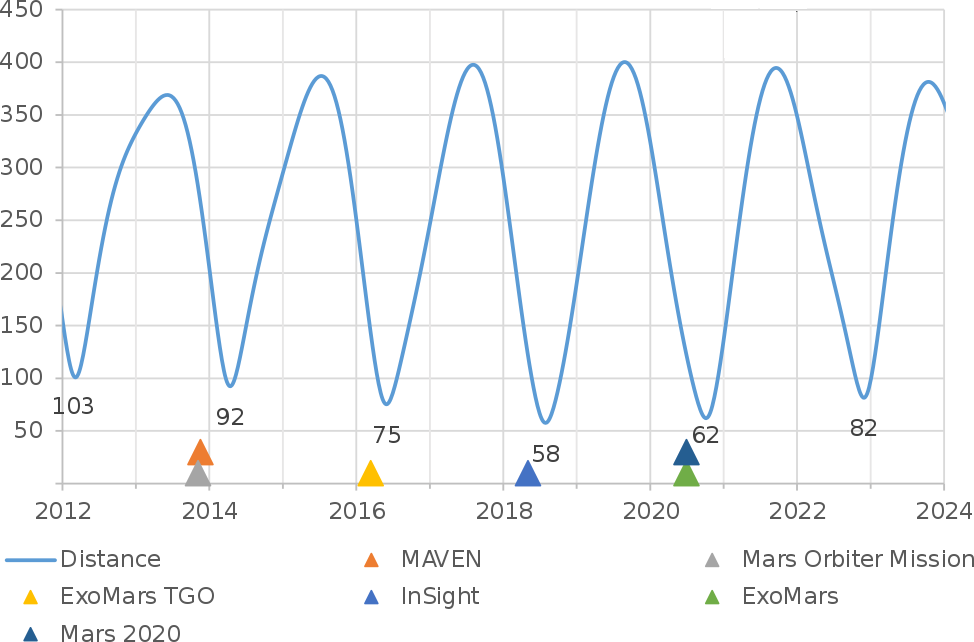
\includegraphics[width=0.5\linewidth]{sections/state-of-the-art/planned-missions/plots/mars-distance-from-earth.png}\\
  \caption[Spacecraft launches and Mars distance from Earth]
          {Spacecraft launches and Mars distance from Earth (Gm). Data source: HORIZONS System, JPL, NASA.}
  \label{fig:mars-distance-from-earth}
\end{figure}

At the time of writing this thesis, two rover missions are set to be launched during the next window: \ac{NASA}'s Mars 2020 rover, shown in Figure \ref{fig:sub:planned-mission-rover-mars2020}, and the \ac{ESA}/Roscosmos' ExoMars Rosalind Franklin rover, shown in Figure \ref{fig:sub:planned-mission-rover-exomars}.

\vspace{0.5cm}

\begin{figure}[h]
\captionsetup[subfigure]{justification=centering}
\vspace{-2ex}
	\centering
    %% setup sizes
    \setlength{\graphicsHeight}{50mm}
    %% kill hyper-link highlighting
    \hypersetup{hidelinks=true}%
    %% the figures
	\begin{subfigure}[t]{0.65\textwidth}
        \centering
		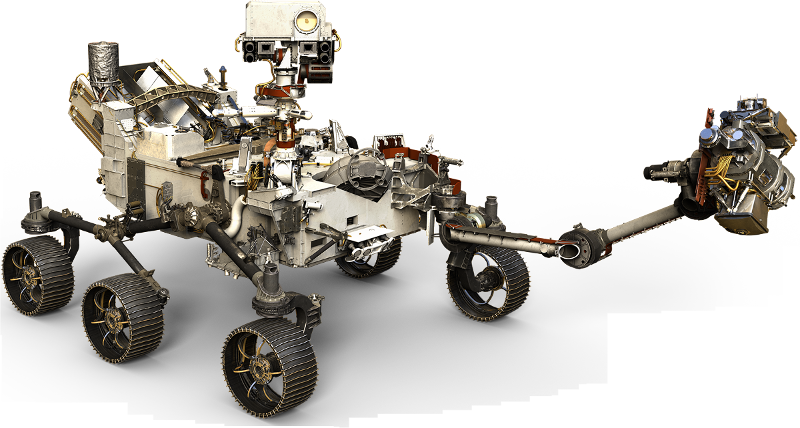
\includegraphics[height=\graphicsHeight]{sections/state-of-the-art/planned-missions/images/rover-mars2020.png}
		\subcaption{Mars 2020}
		\label{fig:sub:planned-mission-rover-mars2020}
	\end{subfigure}\hfill
	\begin{subfigure}[t]{0.35\textwidth}
        \centering
		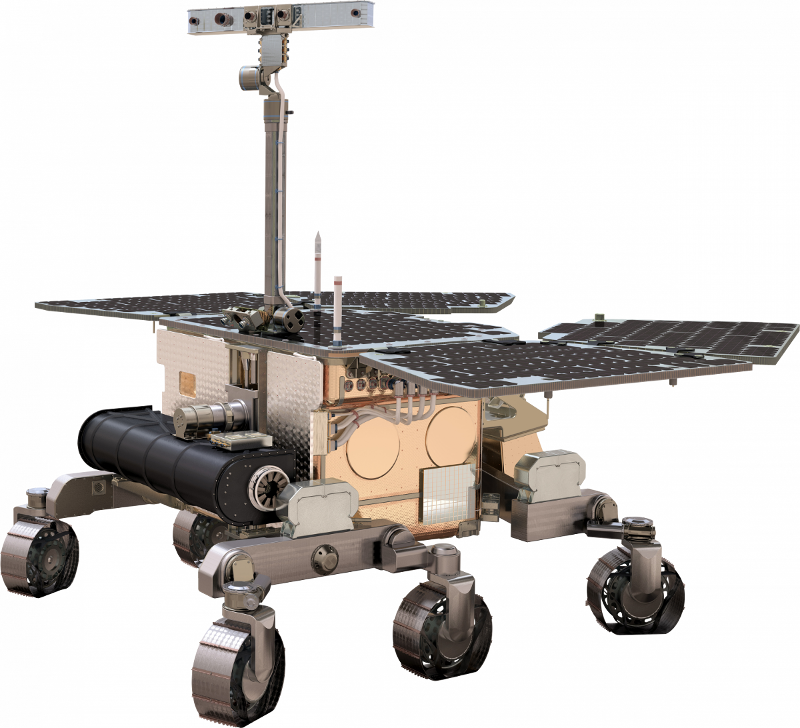
\includegraphics[height=\graphicsHeight]{sections/state-of-the-art/planned-missions/images/rover-exomars.png}
		\subcaption{Rosalind Franklin}
		\label{fig:sub:planned-mission-rover-exomars}
	\end{subfigure}
	\caption[Planned rover missions]
            {Planned rover missions. Mars 2020 is part of \ac{NASA}'s \ac{MEP}. Rosalind Franklin is part of the international ExoMars programme led by \ac{ESA} and Roscosmos}
	\label{fig:planned-mission-rovers}
\vspace{-2ex}
\end{figure}

\subsection{Mars 2020}
\label{sec:StateOfTheArt:PlannedMissions:Mars2020}

Mars 2020 is part of \ac{NASA}'s \ac{MEP}. Much of its design is based on heritage from the Curiosity mission. Its power system is identical to that of Curiosity in that it is equipped with a \ac{MMRTG} that will provide approximately \SI{110}{\watt} of electrical power at \ac{BOL}, declining by a few percent per year \citepower{Mars2020ElecticalPower}. Its two \ac{Li-ion} batteries are also identical to that of Curiosty and was previously elaborated on in Section \ref{sec:StateOfTheArt:PastAndOngoingMissions:Rovers}.

\subsection{Rosalind Franklin}
\label{sec:StateOfTheArt:PlannedMissions:RosalindFranklin}

Rosalind Franklin is part of the international ExoMars programme led by \ac{ESA} and Roscosmos. Its \ac{SA} is designed to generate up to \SI{1200}{\watt\hour} of energy \citepower{SaftPressRelease}. The \ac{SA} power output requirements are:

\begin{itemize}
    \item \ac{BOL}: $P_{max} > \SI{261}{\watt}$ under \SI{471}{Wm^{-2}}, \SI{-26}{\celsius}, and one string fail.
    \item \ac{EOL}: $P_{max} > \SI{131}{\watt}$ under \SI{358}{Wm^{-2}}, \SI{-52}{\celsius}, \SI{34}{\percent} dust coverage, and one string fail plus losses.
\end{itemize}

Test results detailed in \citepower{Riva2019} have measured \ac{SA} performances of $P_{max} = \SI{277}{\watt}$ for \ac{BOL} and $P_{max} = \SI{133.4}{\watt}$ for \ac{EOL}. The rover's battery cells are arranged in a 8s3p configuration and have an operational temperature range of \SI{-40}{\celsius} to +\SI{85}{\celsius} \citepower{EDN}. The rover is equipped with \acp{RHU} in order to maintain its internal temperature above \SI{-40}{\celsius}. The \ac{Li-ion} battery cells are manufactured by Saft and have the following specifications:

\begin{itemize}
    \item Nominal voltage: 3.65 \si{\volt}.
    \item Voltage range: 2.5‒\SI{4.2}{\volt}.
    \item Nameplate capacity: \SI{5.6}{\ampere\hour}.
    \item Nameplate energy:
    \begin{itemize}
        \item \ac{BOL}: \SI{1140}{\watt\hour}  under +\SI{50}{\celsius}, \SI{50}{\percent}. \ac{SOC}.
        \item End of cruise: \SI{980}{\watt\hour} under +\SI{40}{\celsius}, \SI{50}{\percent} \ac{SOC}.
        \item \ac{EOL}: \SI{790}{\watt\hour} under \SI{-20}{\celsius}, \SI{40}{\percent}. \ac{DOD}.
    \end{itemize}
\end{itemize}

The battery characterstics taken from \citepower{Amos2017} are as follow:

\begin{itemize}
    \item Operating voltage: 21‒\SI{29.4}{\volt}.
    \item Mass: $<$ \SI{10.5}{\kilo\gram}.
    \item Charge current:
    \begin{itemize}
        \item T $>$ \SI{0}{\celsius}: up to \SI{3}{\ampere}.
        \item T $<$ \SI{0}{\celsius}: up to \SI{5.2}{\ampere}.
    \end{itemize}
    \item Discharge current:  up to \SI{15}{\ampere}.
\end{itemize}


\section{Photovoltaics and Energy Storage}
\label{sec:StateOfTheArt:PhotovoltaicsAndEnergyStorage}
\subsection{Solar Cells}
At the time of writing this thesis, the InSight lander is the most recent solar powered mission currently operating on the Martian surface. On its first Sol, it generated a record breaking \SI{4.6}{\kilo\watt\hour} of energy. Its``UltraFlex'' \acp{SA} are manufactored by Orbital ATK.

\subsubsection{Triple Junction}
The ``UltraFlex'' \acp{SA} are made from from SolAero \ac{ZTJ} \ac{InGaP}/\ac{InGaAs}/\ac{Ge} space solar cells that boast a \SI{29.5}{\percent} \ac{BOL} efficiency at maximum power point for \ac{AM0} and \SI{135.3}{\milli\watt/\centi\meter^{2}} \citepower{SolAeroZTJDataSheet}. Similar solar cells with idential efficiencies are also available from other manufacturers such as Emcore \citepower{EmcoreZTJDataSheet}. \ac{TJ} \ac{GaAs} junction solar cells manufactured by AzureSpace advertise an average effeciency of \SI{29.5}{\percent} at \SI{1367}{\watt/\centi\meter^{2}} and \SI{29.8}{\percent} at \SI{1353}{\watt/\centi\meter^{2}} for \ac{AM0}, \SI{28}{\celsius} \citepower{AzureSpaceTJDataSheet}.

\subsubsection{Quadruple Junction}
\ac{QJ} solar cells of type \ac{AlInGaP}/\ac{AlInGaAs}/\ac{InGaAs}/\ac{Ge} on \ac{Ge} substrate manufactured by AzureSpace have an average efficiency of \SI{31.8}{\percent} at \ac{BOL} for \ac{AM0}, \SI{1367}{\watt/\centi\meter^{2}}, \SI{25}{\celsius} \citepower{AzureSpaceQJDataSheet}. \ac{QJ} solar cells with high theoretical efficiency of \SI{47.2}{\percent} have been proposed in \citepower{Hossain2016} as well as up to \SI{50}{\percent} efficiency with \ac{InGaP}/\ac{InGaAs}/\ac{InGaAsN}/\ac{Ge} in \citepower{Bestam2016}.

\subsubsection{Inverted Metamorphic Multi Junction}
Space-grade \ac{IMM} solar cells manufactured by SolAero have a typical \ac{BOL} efficiency of \SI{32}{\percent} at maximum power point for \ac{AM0}, \SI{135.3}{\milli\watt/\centi\meter^{2}}, and \SI{28}{\celsius} \citepower{SolAeroIMMDataSheet}. Series-connected \ac{5J} and \ac{6J} concentrator solar cell strategies have been proposed in \citepower{Geisz2017} as an extension to \ac{QJ} \ac{IMM} for a potential to exceed \SI{50}{\percent} efficiency.

\subsection{Battery Cells}
The battery cell presented in this section were selected from manufacturers that provided cells for InSight, Mars 2020, and Rosalind Franklin.

\subsubsection{Yardney EaglePicher}
The \ac{SOA} with Yardney EaglePicher are \ac{NCA} \ac{Li-ion} space battery cells with nominal capacity options of \SI{43}{\ampere\hour} or \SI{60}{\ampere\hour} at C/5 and \SI{20}{\celsius}. They share the same voltage range from 3 to \SI{4.1}{\volt} with a nominal voltage of \SI{3.6}{\volt}. The following specifications are taken from \citepower{EaglePicher43AhBatteryCell} and are specific to the \SI{43}{\ampere\hour} cells:

\begin{itemize}
    \item Energy density: \SI{378}{\watt\hour/l}.
    \item Specific energy: \SI{153}{\watt\hour/\kilo\gram}.
    \item Operating temperature: \SI{-20}{\celsius} to +\SI{60}{\celsius}.
    \item Charging method: constant \SI{21.5}{\ampere} (0.5C) current to \SI{4.1}{\volt}. and a constant voltage  \SI{4.1}{\volt} to 0.86 \si{\ampere} (C/50).
    \item Discharge rates with a maximum constant curent of \SI{200}{\ampere}.
\end{itemize}

The following specifications are from \citepower{EaglePicher60AhBatteryCell} and are specific to the \SI{60}{\ampere\hour} cells:

\begin{itemize}
    \item Energy density: \SI{393}{\watt\hour/l}.
    \item Specific energy: \SI{160}{\watt\hour/\kilo\gram}.
    \item Operating temperature: \SI{-20}{\celsius} to +\SI{40}{\celsius}.
    \item Charging method: constant \SI{12}{\ampere} (0.2C) current to \SI{4.1}{\volt} and a constant voltage \SI{4.1}{\volt} to \si{1.2}{\ampere} (C/50).
    \item Discharge rates with a maximum constant curent of \SI{250}{\ampere}.
\end{itemize}

\subsubsection{Saft}
Saft's prismatic MP and cylindrical VL rechargeable \ac{Li-ion} battery cells have the lowest temperature performance for charging, operating down to \SI{-50}{\celsius}. The following specifications are taken from \citepower{SaftSpaceBatteryCell}:

\begin{itemize}
  \item Nominal voltage: 3.6‒\SI{3.75}{\volt}.
  \item Energy density: up to \SI{385}{\watt\hour/l}.
  \item Specific energy: \SI{180}{\watt\hour/\kilo\gram}.
  \item Power range: up to \SI{1}{\kilo\watt/\kilo\gram}.
  \item Capacity range: 2.6‒\SI{7.0}{\ampere\hour}.
  \item Operating temperature: \SI{-20}{\celsius} to +\SI{60}{\celsius} for charge and \SI{-50}{\celsius} to +\SI{60}{\celsius} for discharge.
\end{itemize}


%\section{Summary and Conclusion}
%\label{sec:StateOfTheArt:SummaryAndConclusion}
%\todo[inline]{\textbf{TODO:} Write summary and conclusion for this chapter.}

%%%%%%%%%%%%%%%%%%%%%%%%%%%%%%%%%%%%%%%%%%%%%%%%%%%%%%%


%%%%%%%%%%%%%%%%%%%%%%%%%%%%%%%%%%%%%%%%%%%%%%%%%%%%%%%
\chapter{The Martian Environment}
%\shinyChapterQuote{}
\label{sec:MartianEnvironment}
%\acresetall                 %% reset all acronym abbreviations and write first appearance long
%\acused{CAD}
\acused{DoF}
\acused{EEPROM}
\acused{FPGA}
\acused{GPS}
\acused{HD}
\acused{LED} %%define ackronyms that are "common sense"
%\input{sections/martian-environment/references.tex}



\section{Dust}
\label{sec:MartianEnvironment:Dust}
%\input{sections/s.tex}

% Martian Season - start with images
% Regolith, dust, and craters, other elements
% Settle with locations DTMS

Great dust storms (area > 10e6 km2) occur with a yearly probability of 30\% to 80\%. \citepower{Kerslake1999}

Local dust storms (area < 10e6 km2) occur with a 5\% probability in Mars equatorial regions and have only a minor impact on seasonal insulation due to their limited size, duration (a few days), and moderate OD (~1). \citepower{Kerslake1999}

the dust accumulation rate is assumed to be 5\% of that measured by Pathfinder \citepower{Kerslake1999}

Losses from lander vehicle shadowing and terrain masking are not yet modeled pending better definitions of lander configuration and landing sites. \citepower{Kerslake1999}

For desirable near-equatorial landing sites (not in canyons), shadowing and terrain masking losses will be small. This is due to high sun angles (that create short shadows) and the large component of diffuse solar insolation near dusk and dawn (when the terrain masking effect is largest). \citepower{Kerslake1999}


\section{Dust Storms}
\label{sec:MartianEnvironment:DustStorms}
%\input{sections/s.tex}

%%%%%%%%%%%%%%%%%%%%%%%%%%%%%%%%%%%%%%%%%%%%%%%%%%%%%%%

%%%%%%%%%%%%%%%%%%%%%%%%%%%%%%%%%%%%%%%%%%%%%%%%%%%%%%%
\chapter{Power and Energy Predictions}
%\shinyChapterQuote{I have the power!}
%  {He-Man}
\label{sec:PowerAndEnergyPredictions}
\section{Performance Ratio}
\label{sec:PowerAndEnergyPredictions:PerformanceRatio}
Power and energy calculations take into account solar cell performance ratio $PR$, also known as the coefficient for losses. $PR$ components are taken from Mars \ac{PV} literature:

\begin{enumerate}[(a)]
  \item\label{itm:pr:perm_loss}After deployment, \SI{5}{\percent} permanent dust power loss \citepower{McNatt2016}.
  \item\label{itm:pr:temp}Solar cell efficiency varies by \SI{3}{\percent} due to changing temperature and red-shift spectral losses through the day time-period \citepower{Kerslake1999}.
  \item\label{itm:pr:deposition}Dust deposition degrade the performance at a rate of \SI{0.28}{\percent} per sol during the initial 30 Sols of a mission and long-term degradation is about \SI{0.14}{\percent} per sol \citepower{Landis2004}.
  \item\label{itm:pr:saturation}Dust performance degradiation saturates at about \SI{30}{\percent} \citepower{Stella2005}.
  \item\label{itm:pr:shadowing}Variable shadowing from protruding rover structures \citepower{Stella2005} and terrain masking \citepower{Kerslake1999}.
\end{enumerate}

The components used for \ac{PR} in the daily energy calculations throughout this chapter will initially be made up of degradation coefficients from (\ref{itm:pr:perm_loss}) and (\ref{itm:pr:temp}) where validation against \ac{MER} Opportunity data will use the solar array dust factor reported by the rover rather than those described in (\ref{itm:pr:deposition}) and (\ref{itm:pr:saturation}). Losses from (\ref{itm:pr:shadowing}) and other unaccounted factors will be initially assumed at \SI{5}{\percent} and then iteratively revised along with the solar array dust factor so that the error margin range may be reduced.

Dust deposition induced losses do not perennially degrade the solar cells but fluctuate due to probabilistic dust cleaning events such as encounters with dust devils, storm winds, or even from a steep tilt angle as seen in Figure \ref{fig:image:mer-opportunity-dust-streaks}.

\begin{figure}[h]
  \centering
  \hypersetup{linkcolor=captionTextColor}
  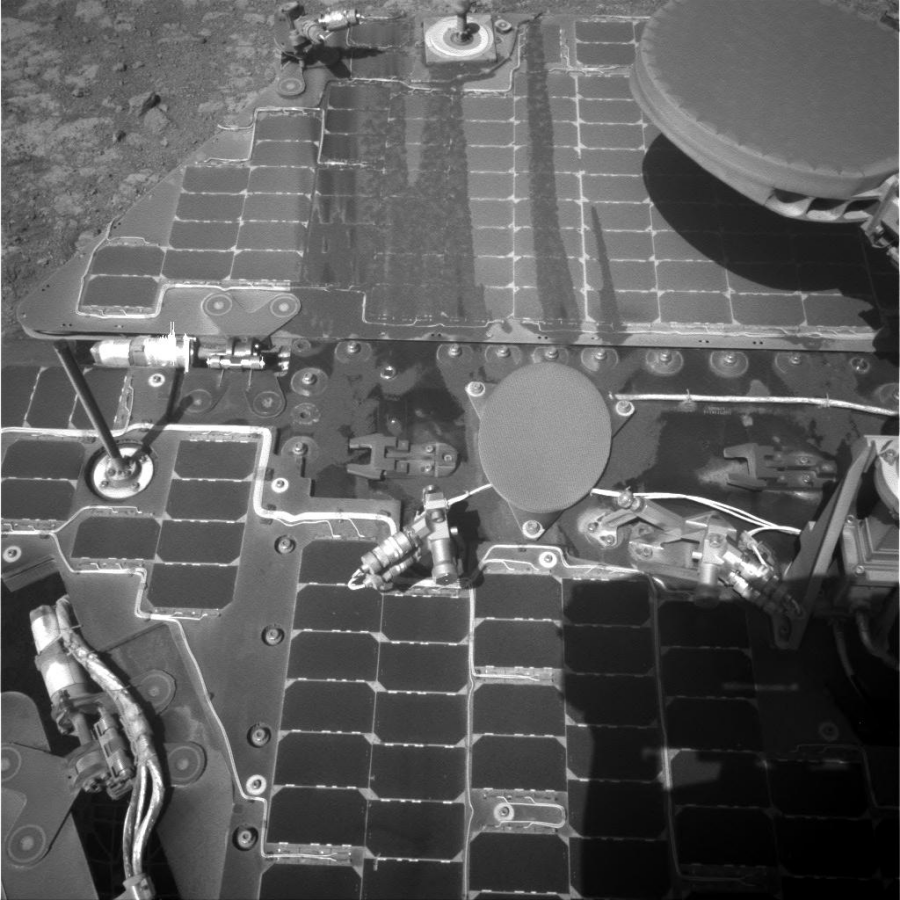
\includegraphics[width=0.4\linewidth]{sections/power-and-energy-predictions/images/mer-opportunity-dust-streaks.png}\\
  \caption[Streak of dust on \ac{MER} Opportunity's rear solar array during a steep tilt]
          {During a forward, uphill drive on Sol 4311 (March 10, 2016), Opportunity's tilt reached \SI{32}{\degree}. Vibrations from wheels slipping against the ground caused dust to streak down from \ac{MER} Opportunity's rear solar array while the rover was steeply tilted. Image taken on Sol 4322 (March 21, 2016). Image: \ac{NASA}/\ac{JPL}-Caltech.}
  \label{fig:image:mer-opportunity-dust-streaks}
\end{figure}
% Source: https://www.nasa.gov/feature/jpl/rover-takes-on-steepest-slope-ever-tried-on-mars

\clearpage
\section{Predictions}
\label{sec:PowerAndEnergyPredictions:Predictions}

The power output $P$ generated from a photovoltaic system is measured in watts (\si{\watt}) and is obtained from the global irradiance $G_{h}$ captured by its solar cells:

\begin{equation}
  \label{eq:SA_power}
  P = A \cdot \eta \cdot G_{h} \cdot PR
\end{equation}

where $A$ is the solar cell coverage area $\eta$ their efficiency.

The generated daily energy output $E$ is measured in watt-hours (\si{\watt\hour}) and is obtained from the daily global insolation $H_{h}$ captured by solar cells:

\begin{equation}
  \label{eq:SA_energy}
  E = A \cdot \eta \cdot H_{h} \cdot PR
\end{equation}

Power and energy calculations for inclined solar arrays are obtained from $G_{\beta}$ and $I_{\beta}$. They are denoted as $P_{\beta}$ and $E_{\beta}$ respectively:

\begin{equation}
  \label{eq:SA_slope_power}
  P_{\beta} = A \cdot \eta \cdot G_{\beta} \cdot PR
\end{equation}


\begin{equation}
  \label{eq:SA_slope_energy}
  E_{\beta} = A \cdot \eta \cdot H_{\beta} \cdot PR
\end{equation}

It is worth emphasizing the difference between \ac{PV} cell, panel/module, and array surface areas in order to emphasize the correct parameter when calculating generated power and energy. \ac{PV} cells are interconnected together in a package called a panel, or module, which is then wired in series and parallel into a PV array. The interconnections between cells and wiring between panels introduce cell coverage gaps from which no power is generated. As such, considering panel or array rather than cell surface area for power and energy calculations would result in over-estimated values. By way of example, we consider the solar arrays on MER rovers in Figure \ref{fig:image:mer-solar-arrays} which is made up of a total of 499 cells: 165 on the port wing, 167 on the starboard wing, 102 on the stern, and 65 on the body. A cell's dimension is $\SI{3.95}{\centi\meter} \times \SI{6.89}{\centi\meter}$ with two cropped corners. This provides an active area of \SI{26.6}{\centi\meter\squared} thus the solar cell coverage area is $499 \times \SI{26.6}{\centi\meter\squared} = \SI{1.3}{\meter\squared}$.

\todo[inline]{TODO: Source E-mail exchange with Richard C. Ewell (NASA/JPL) for the MER solar cell size.}

\begin{figure}[h]
  \centering
  \hypersetup{linkcolor=captionTextColor}
  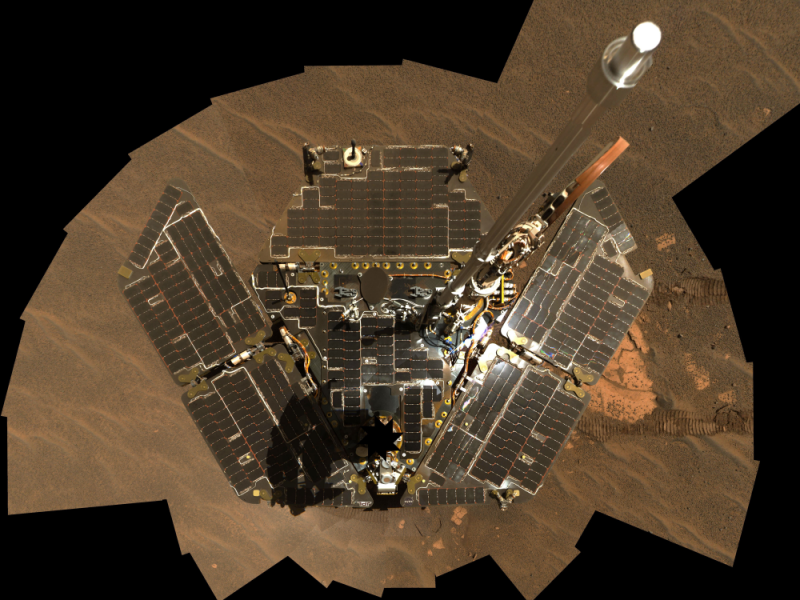
\includegraphics[width=0.8\linewidth]{sections/power-and-energy-predictions/images/mer-solar-arrays.png}\\
  \caption[\ac{MER} solar arrays]
          {\ac{MER} solar arrays. Image: \ac{NASA}/\ac{JPL}-Caltech/Cornell.}
  \label{fig:image:mer-solar-arrays}
\end{figure}
% Source: https://mars.nasa.gov/resources/5852/opportunity-self-portrait/?site=insight

\clearpage
\section{Validation}
\label{sec:PowerAndEnergyPredictions:Validation}

\todo[inline]{TODO: Short intro text? Why are we validating? Explain that the equations we are using were based on Viking Lander data and we need to verify if it is still robust today by validating it against the wealth of data we've accumulated since, specifically with MER Opportunity data which is illustrative of mobile rover missions rather than a stationary lander mission.}

\subsection{Horizontal Surface}
\label{sec:PowerAndEnergyPredictions:Validation:HorizontalSurface}

In order to validate the formulas presented in Section \ref{sec:PowerAndEnergyPredictions:Predictions}, \ac{MER} Opportunity status update parameters were applied to the daily energy calculation presented in Equation \ref{eq:SA_energy}. The following data was scraped from the rover's status update website for Mars years MY29 through MY33:

\begin{enumerate}[(a)]
  \item Sol: the mission's Martian day when the status report was made.
  \item Terrestrial date: the date on Earth when the status report was made.
  \item Atmospheric opacity: the $\tau$ factor introduced in Section \ref{sec:MartianEnvironment:Dust:AtmosphericOpacity}.
  \item Solar Array dust factor: a value between 0 and 1 with the latter represents perfectly clean solar arrays.
  \item Daily energy production: in watt-hours (\si{\watt\hour}).
\end{enumerate}

For the purpose of insolation calculations, the areocentric longitude $L_{s}$ was determined from the terrestrial date based on the process and equations in \citeother{Allison2000}. The resulting predicted energy production was then compared to the rover's reported daily energy production. These are presented for selected Mars years in Figure \ref{fig:plot:mer-energy-production-predicted-vs-reported}.

\begin{figure}[h]
\captionsetup[subfigure]{justification=centering}
\vspace{-2ex}
	\centering
    %% setup sizes
    \setlength{\subfigureWidth}{0.50\textwidth}
    \setlength{\graphicsHeight}{80mm}
    %% kill hyper-link highlighting
    \hypersetup{hidelinks=true}%
    %% the figures
%% 1st row
  	\begin{subfigure}[t]{\subfigureWidth}
      \centering
  		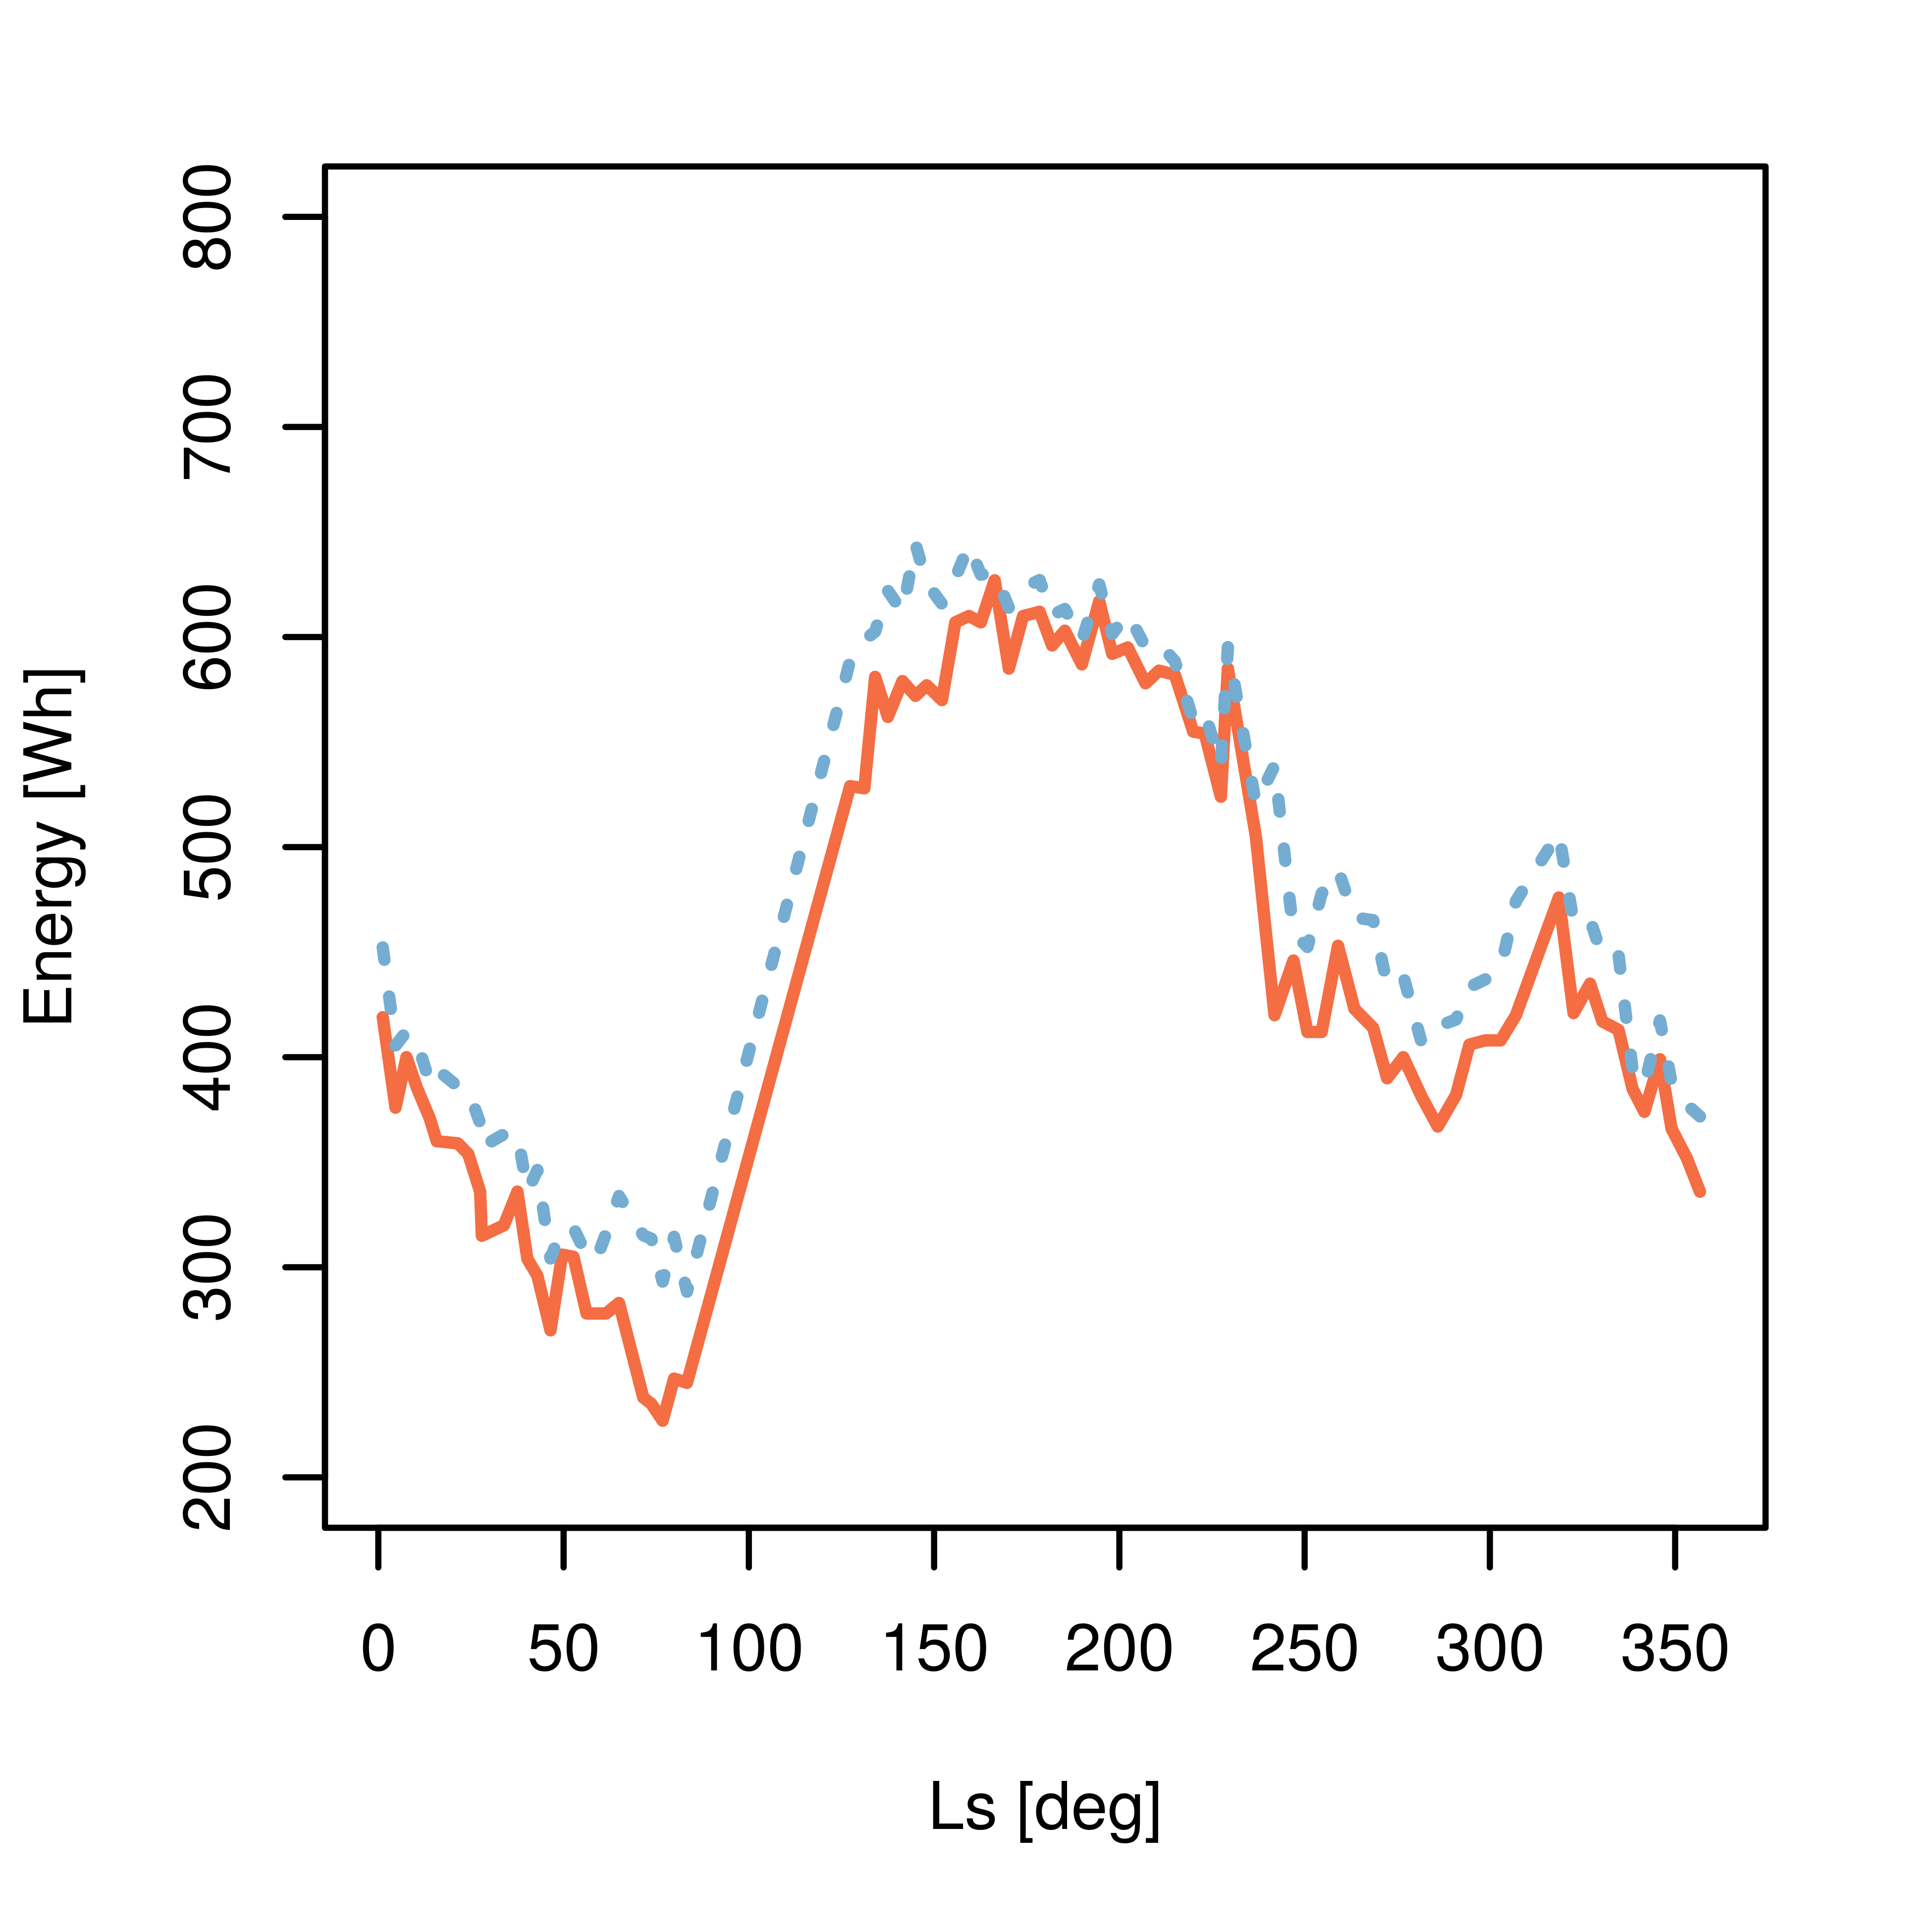
\includegraphics[height=\graphicsHeight]{sections/power-and-energy-predictions/plots/predicted-vs-measured-energy-my29.png}
  		\subcaption{MY29}
  		\label{fig:plot:sub:mer-energy-production-predicted-vs-reported-my29}
  	\end{subfigure}\hfill
    \begin{subfigure}[t]{\subfigureWidth}
      \centering
  		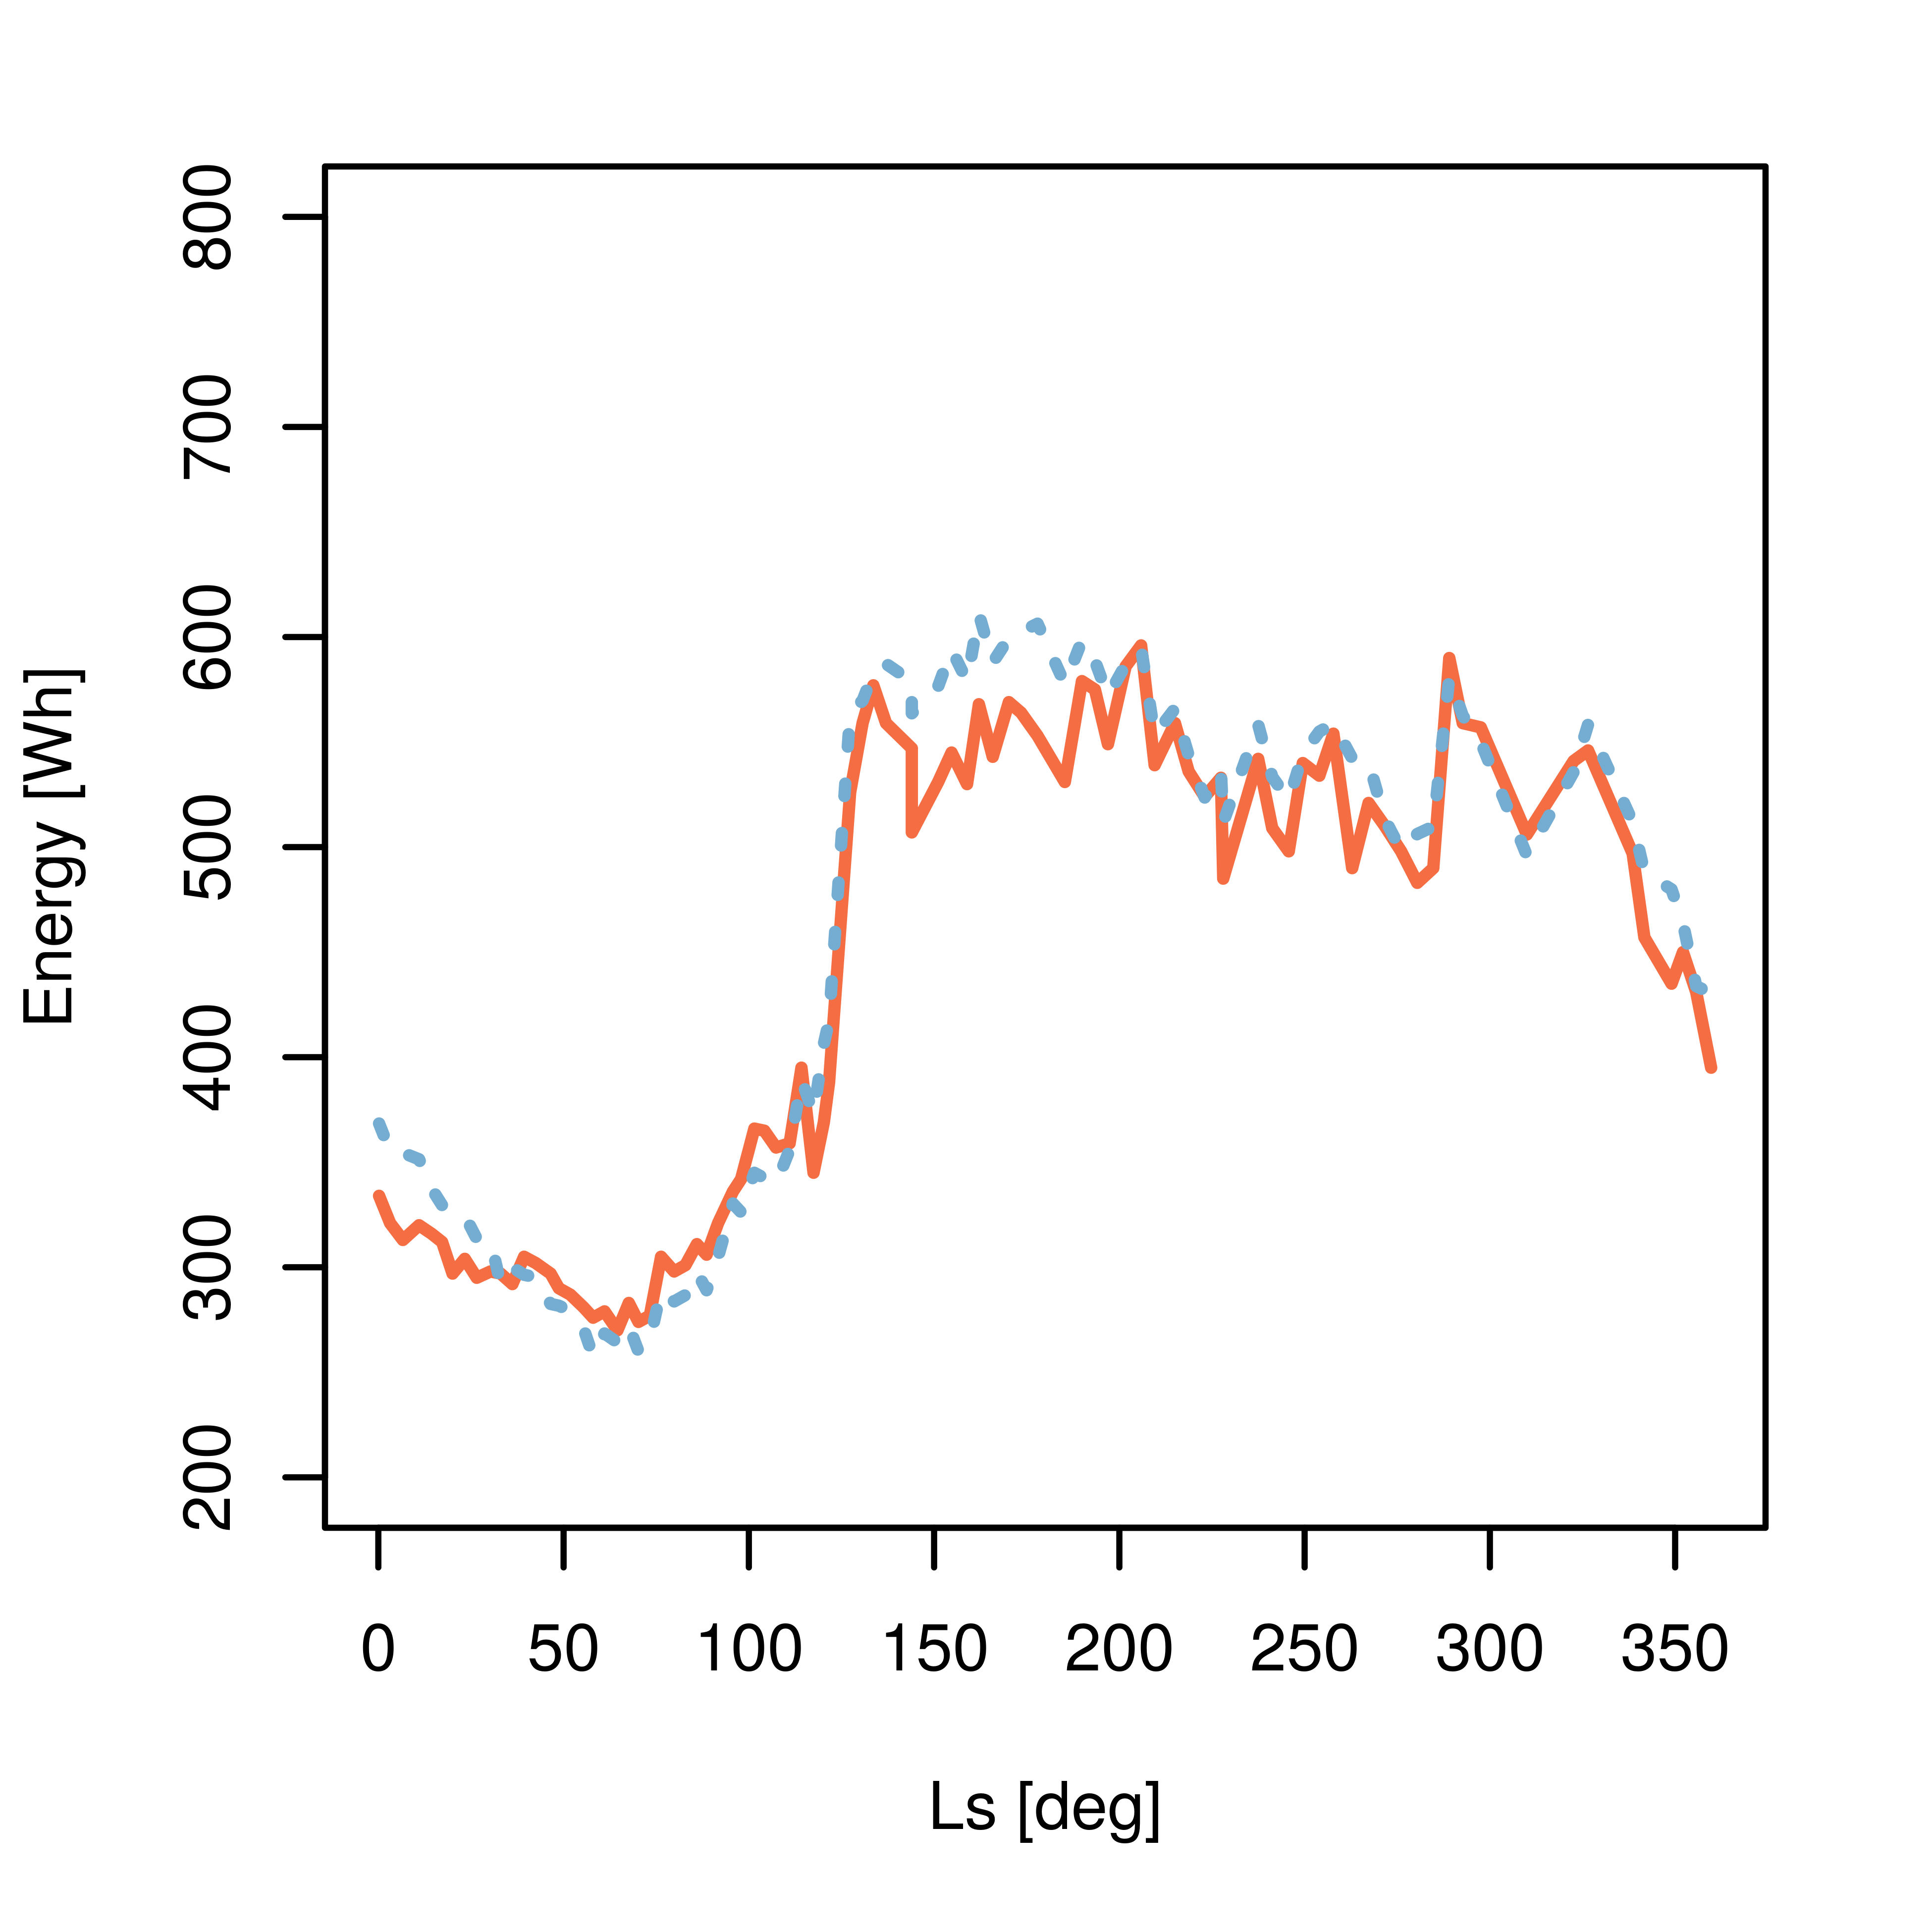
\includegraphics[height=\graphicsHeight]{sections/power-and-energy-predictions/plots/predicted-vs-measured-energy-my30.png}
  		\subcaption{MY30}
  		\label{fig:plot:sub:mer-energy-production-predicted-vs-reported-my30}
  	\end{subfigure}\\[0.8ex]
%% 2nd row
    \begin{subfigure}[t]{\subfigureWidth}
      \centering
  		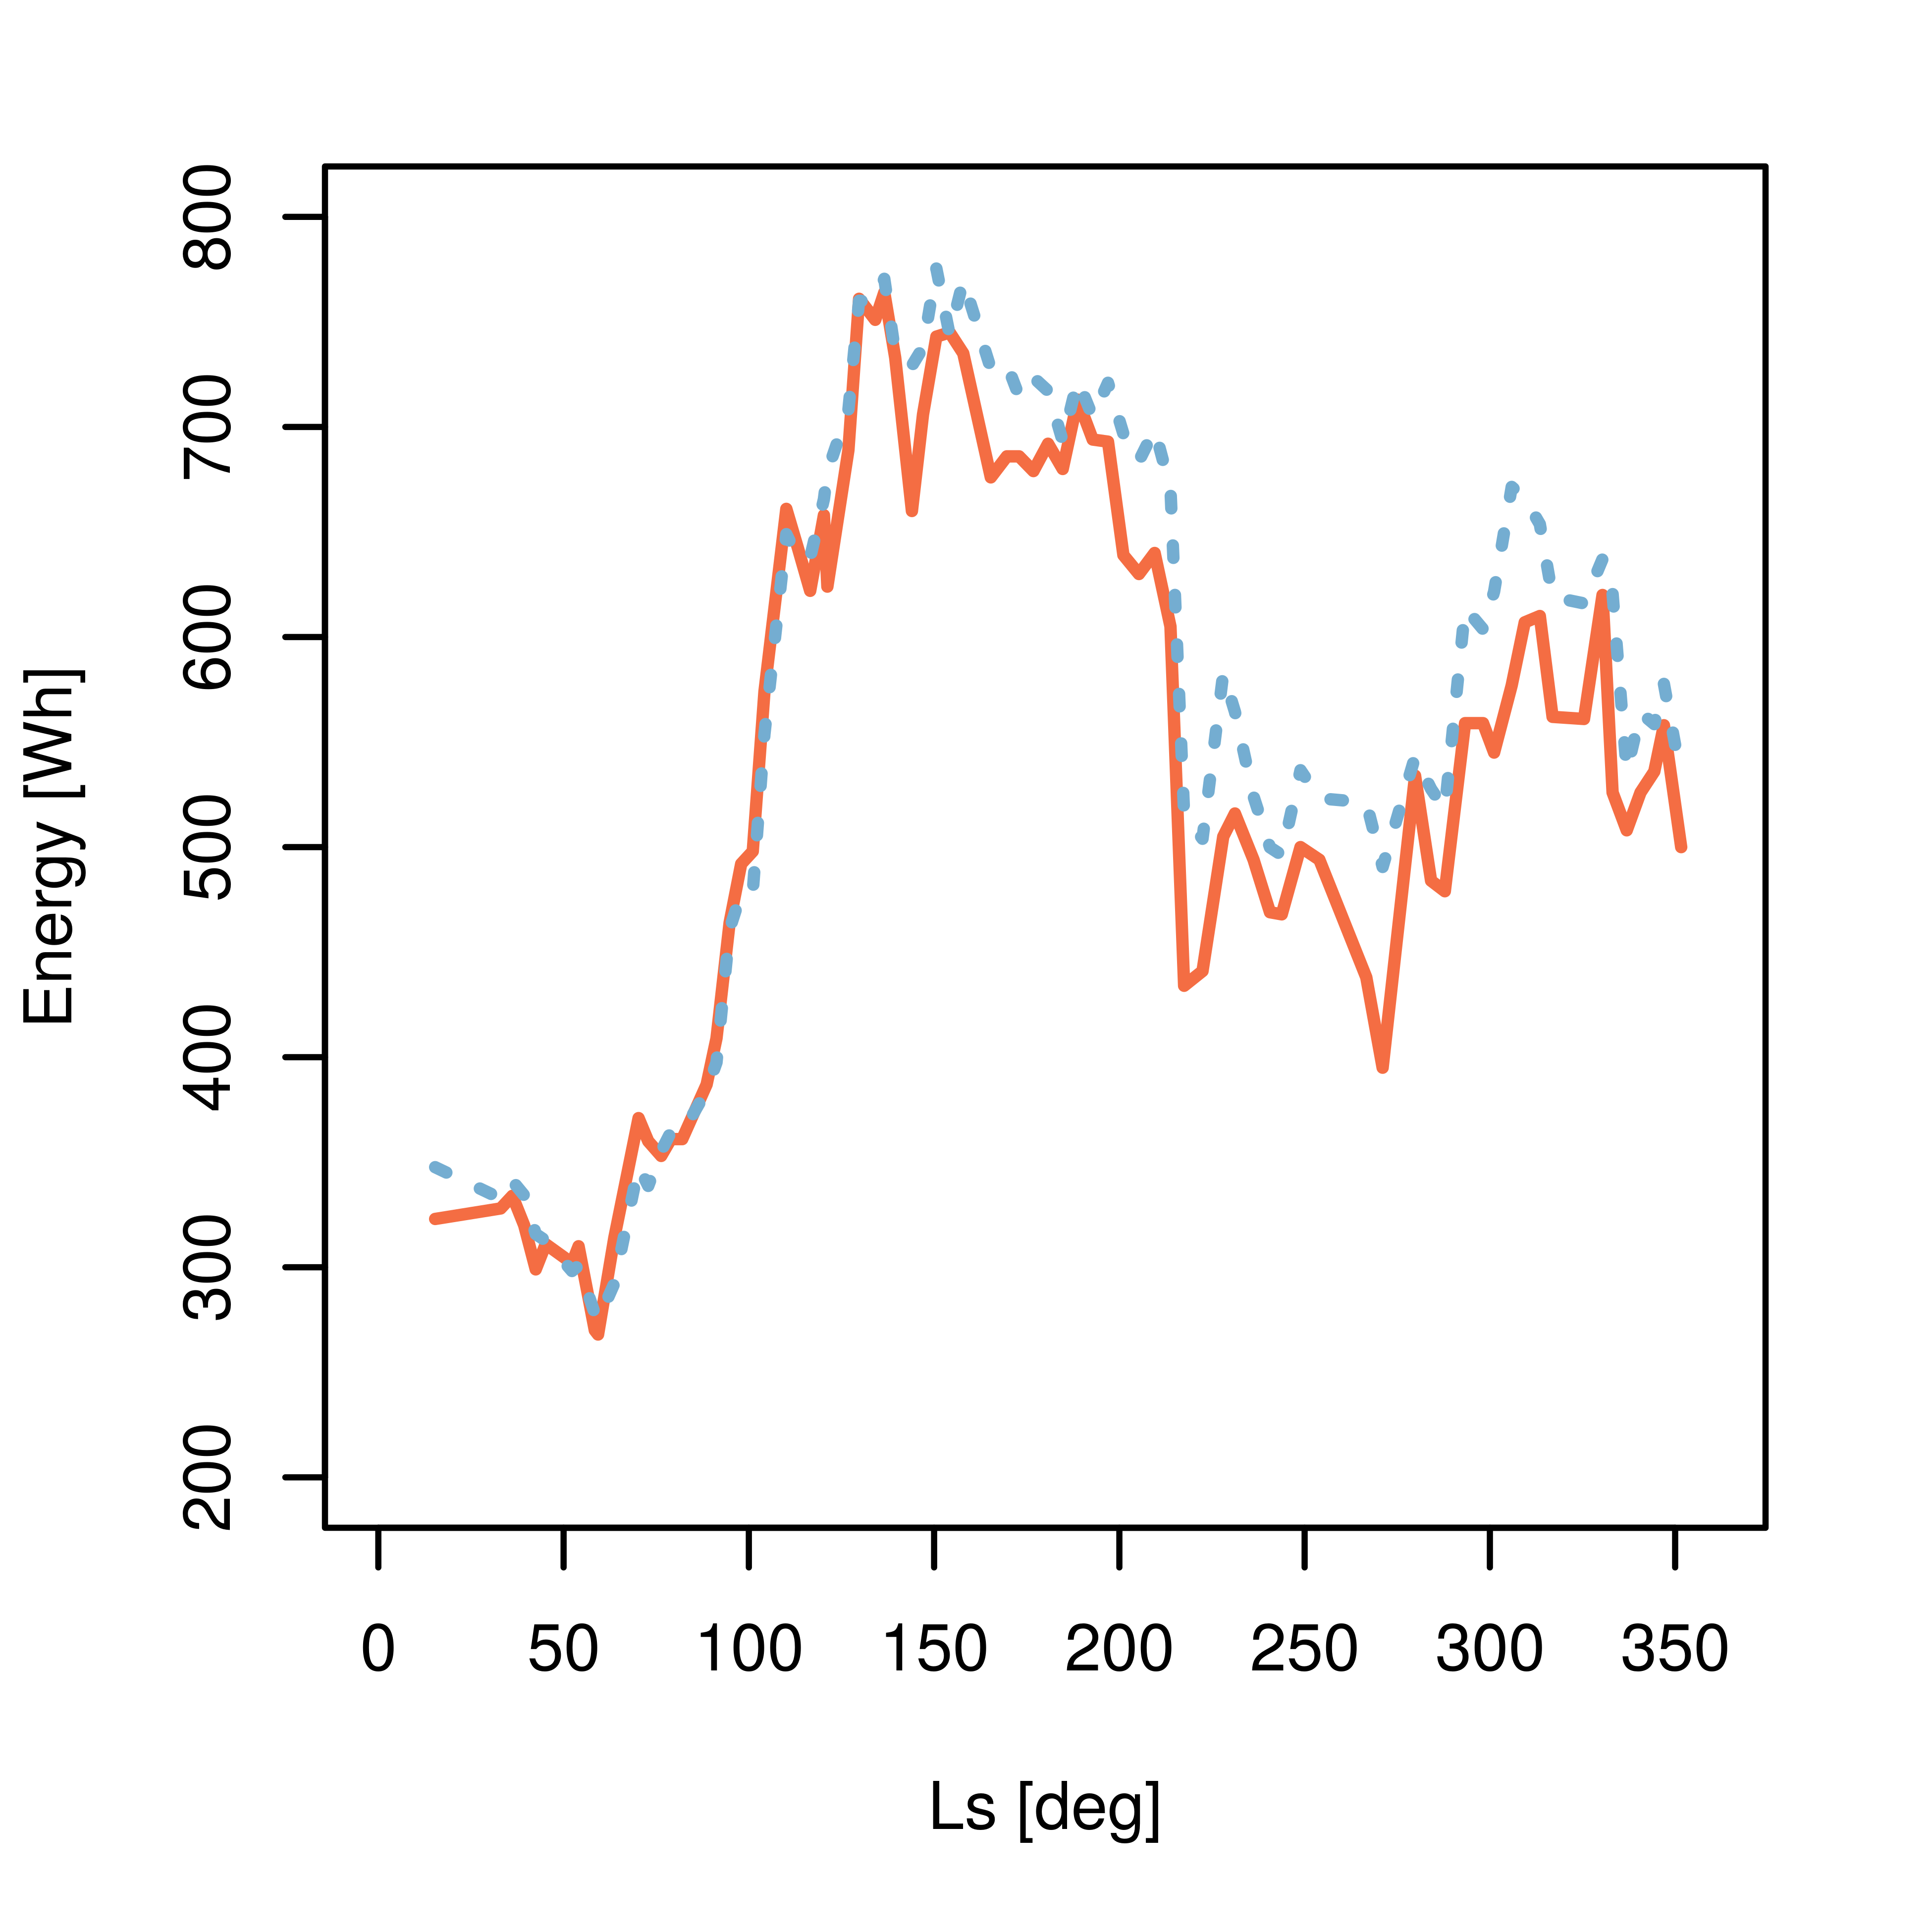
\includegraphics[height=\graphicsHeight]{sections/power-and-energy-predictions/plots/predicted-vs-measured-energy-my32.png}
  		\subcaption{MY32}
  		\label{fig:plot:sub:mer-energy-production-predicted-vs-reported-my32}
  	\end{subfigure}\hfill
	   \begin{subfigure}[t]{\subfigureWidth}
      \centering
  		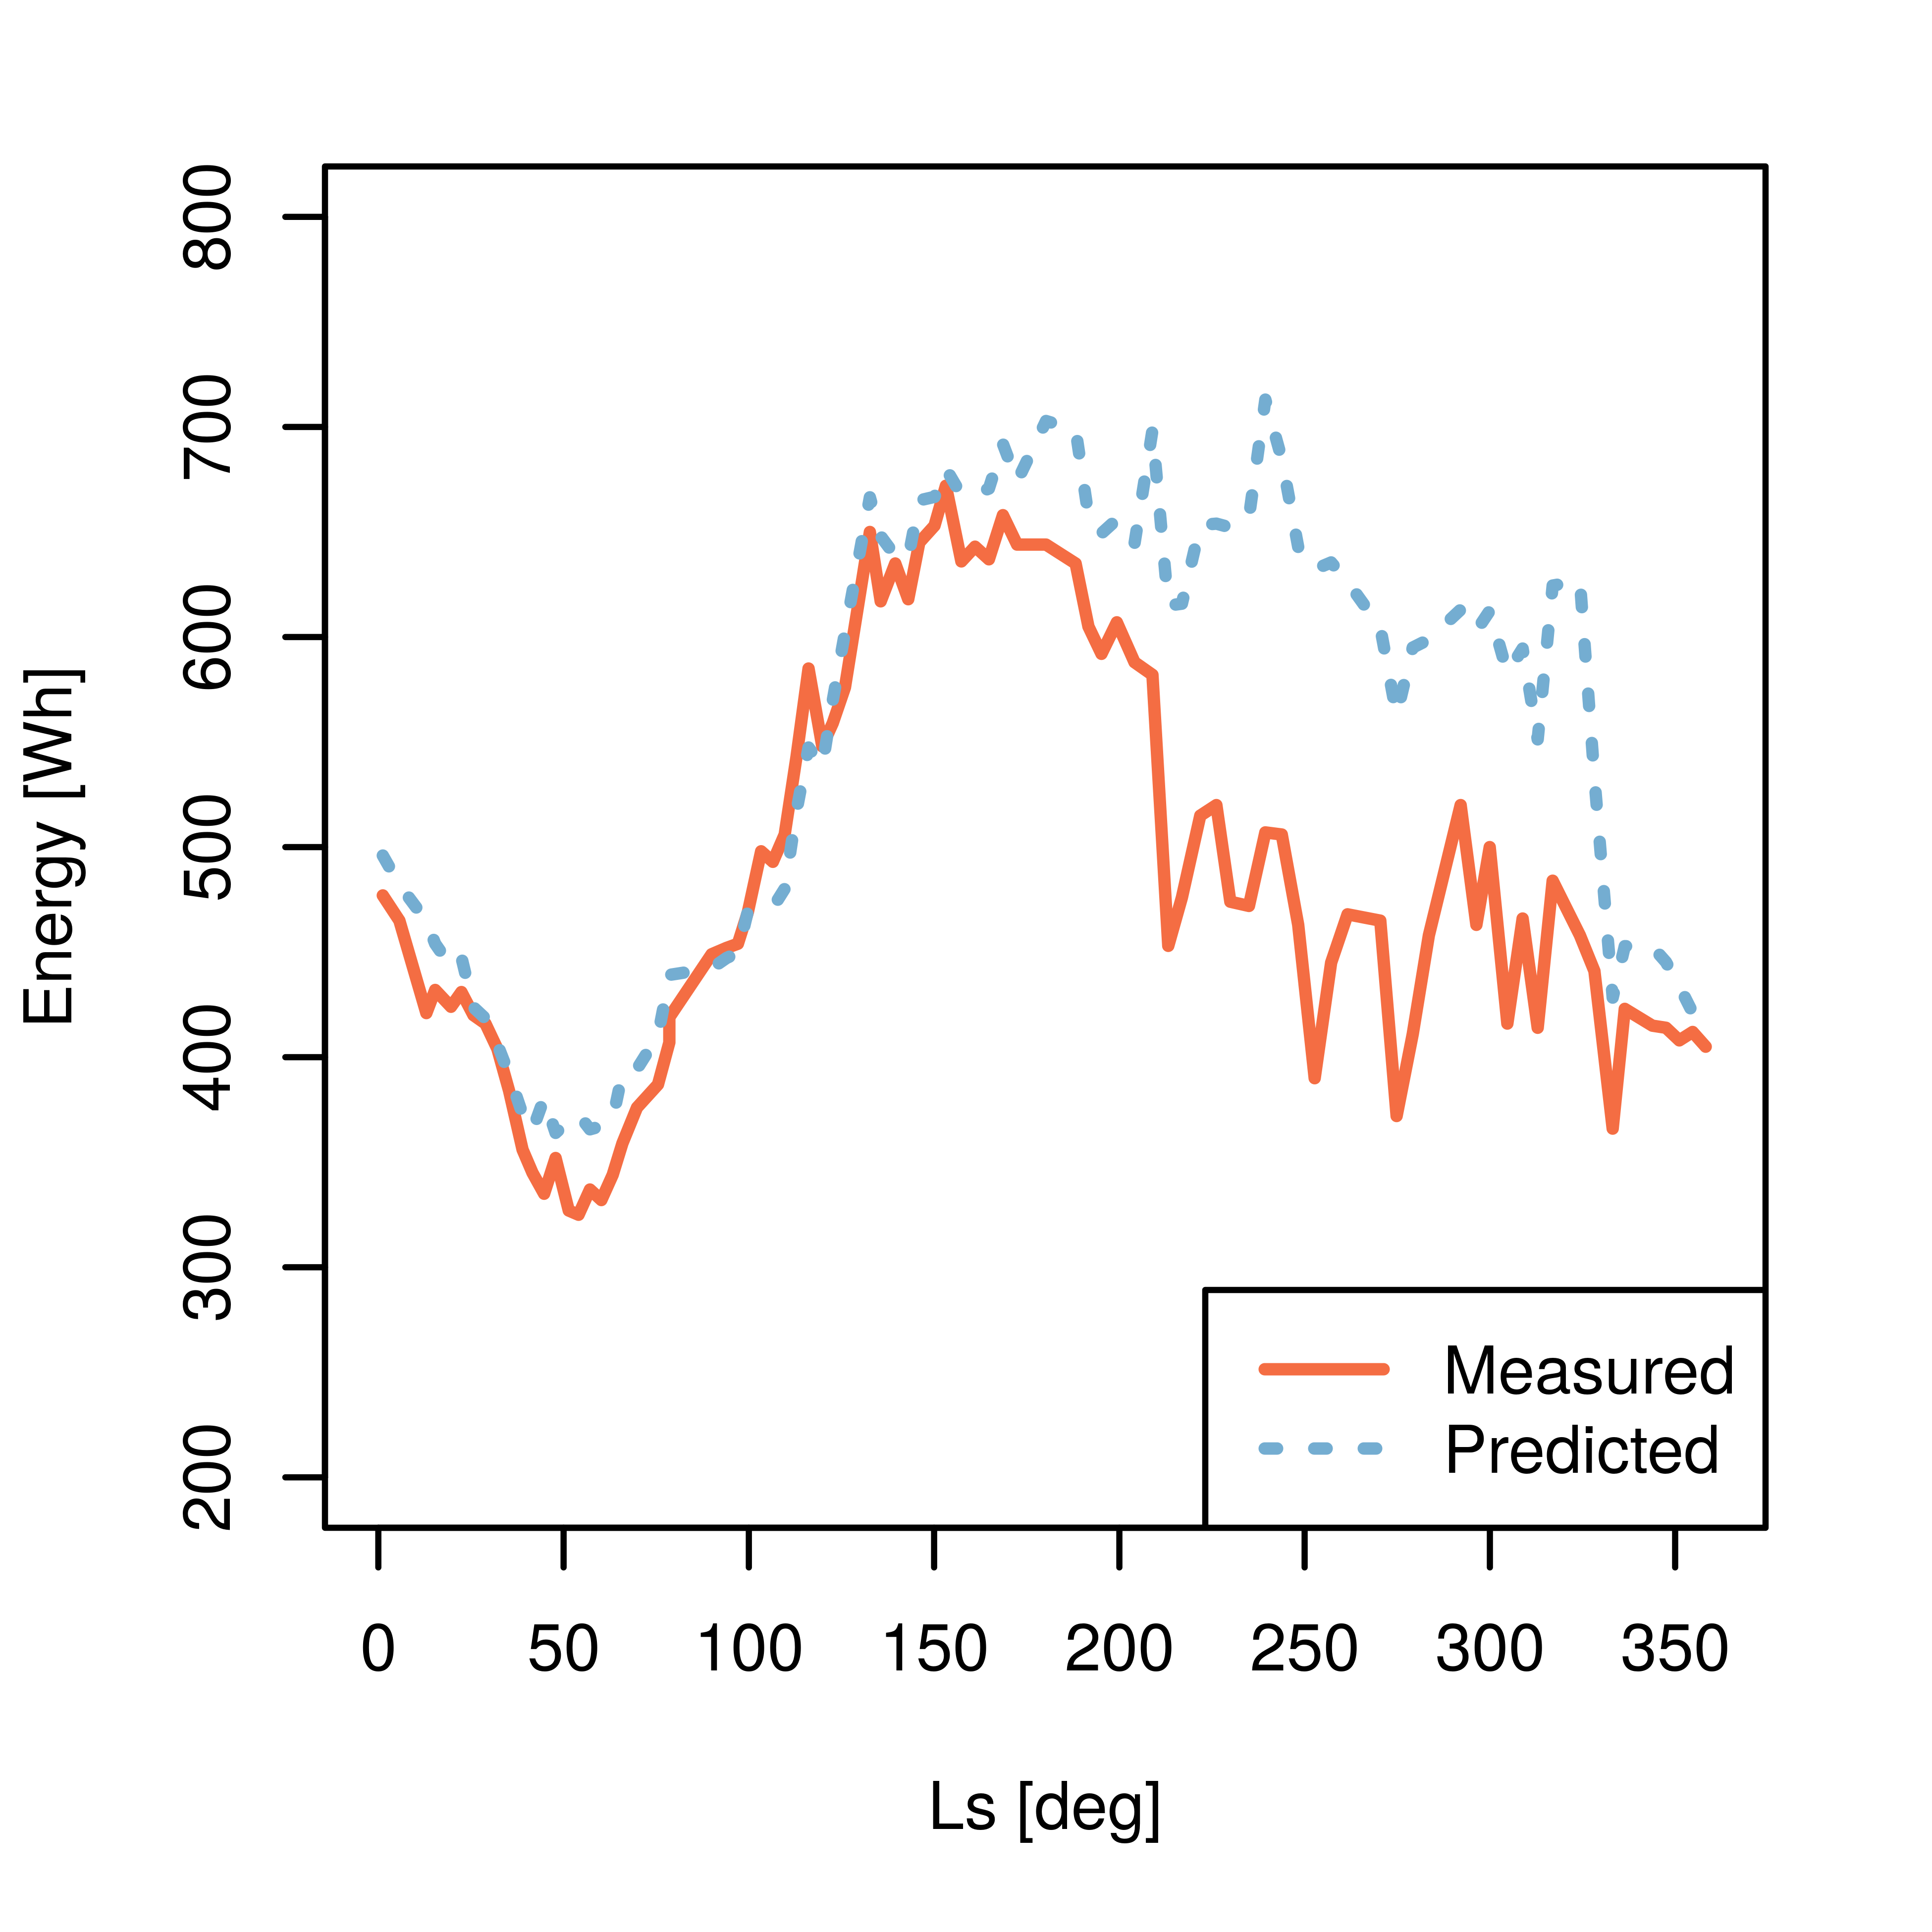
\includegraphics[height=\graphicsHeight]{sections/power-and-energy-predictions/plots/predicted-vs-measured-energy-my33.png}
  		\subcaption{MY33}
  		\label{fig:plot:sub:mer-energy-production-predicted-vs-reported-my33}
	   \end{subfigure}\hfill
    \caption[MER Opportunity PV energy production: predicted vs reported]
            {MER Opportunity PV energy production: predicted vs reported. Not shown are data for MY28 and MY34 which have also been scraped from the rover's status update logs.}
	\label{fig:plot:mer-energy-production-predicted-vs-reported}
\vspace{-2ex}
\end{figure}

\clearpage

A clear outlier is observed during the second half of MY33 in which predicted daily energy productions are much higher than what was reported. This is due to the rover's inclined descent through ``Bitterroot Valley'' during an intensive investigation into a gully at Endeavour Crater's western rim. Energy production predictions with horizontal surface Equation \ref{eq:SA_energy} not suited due to the inclination and orientation of such a descent. Applying Equation \ref{eq:SA_slope_energy} for $E_{\beta}$ would be more applicable. As such, data from MY33 is not considered in the validation exercise for horizontal surfaces.

\todo[inline]{TODO: Include reference to rover update for Bitterroot Valley descent.}
% Source: https://mars.nasa.gov/mer/mission/rover-status/opportunity/recent/all/?y=2016
% Source: https://www.nasa.gov/feature/jpl/rover-takes-on-steepest-slope-ever-tried-on-mars

Not included in Figure \ref{fig:plot:mer-energy-production-predicted-vs-reported} is data for MY34 during which the rover spent most of the year driving down ``Perseverance Valley'' on the west rim of Endeavour Crater. As was the case for MY33, applying Equation \ref{eq:SA_energy} for the MY34 would not be appropriate considering the rover's inclination during descents and is not considered in the validation exercise for horizontal surfaces.

% Source:https://mars.nasa.gov/mer/mission/rover-status/opportunity/recent/all/?y=2017
% Opportunity Remains at Current Location Due to Solar Conjunction
% sols 4787 to 4792, July 12, 2017 - July 17, 2017
% Opportunity entered Perseverance Valley on the west rim of Endeavour crater. The rover is positioned within the valley where she will spend the solar conjunction period.

Divergences from the predicted energy production are presented in Figure \ref{fig:plot:mer-energy-prediction-divergences} from which a -33\%/+7\% error margin range is observed. Negative values indicate predicted daily energy production greater than what was measured and the inverse is indicated by positive values.

\begin{figure}[h]
  \centering
  \hypersetup{linkcolor=captionTextColor}
  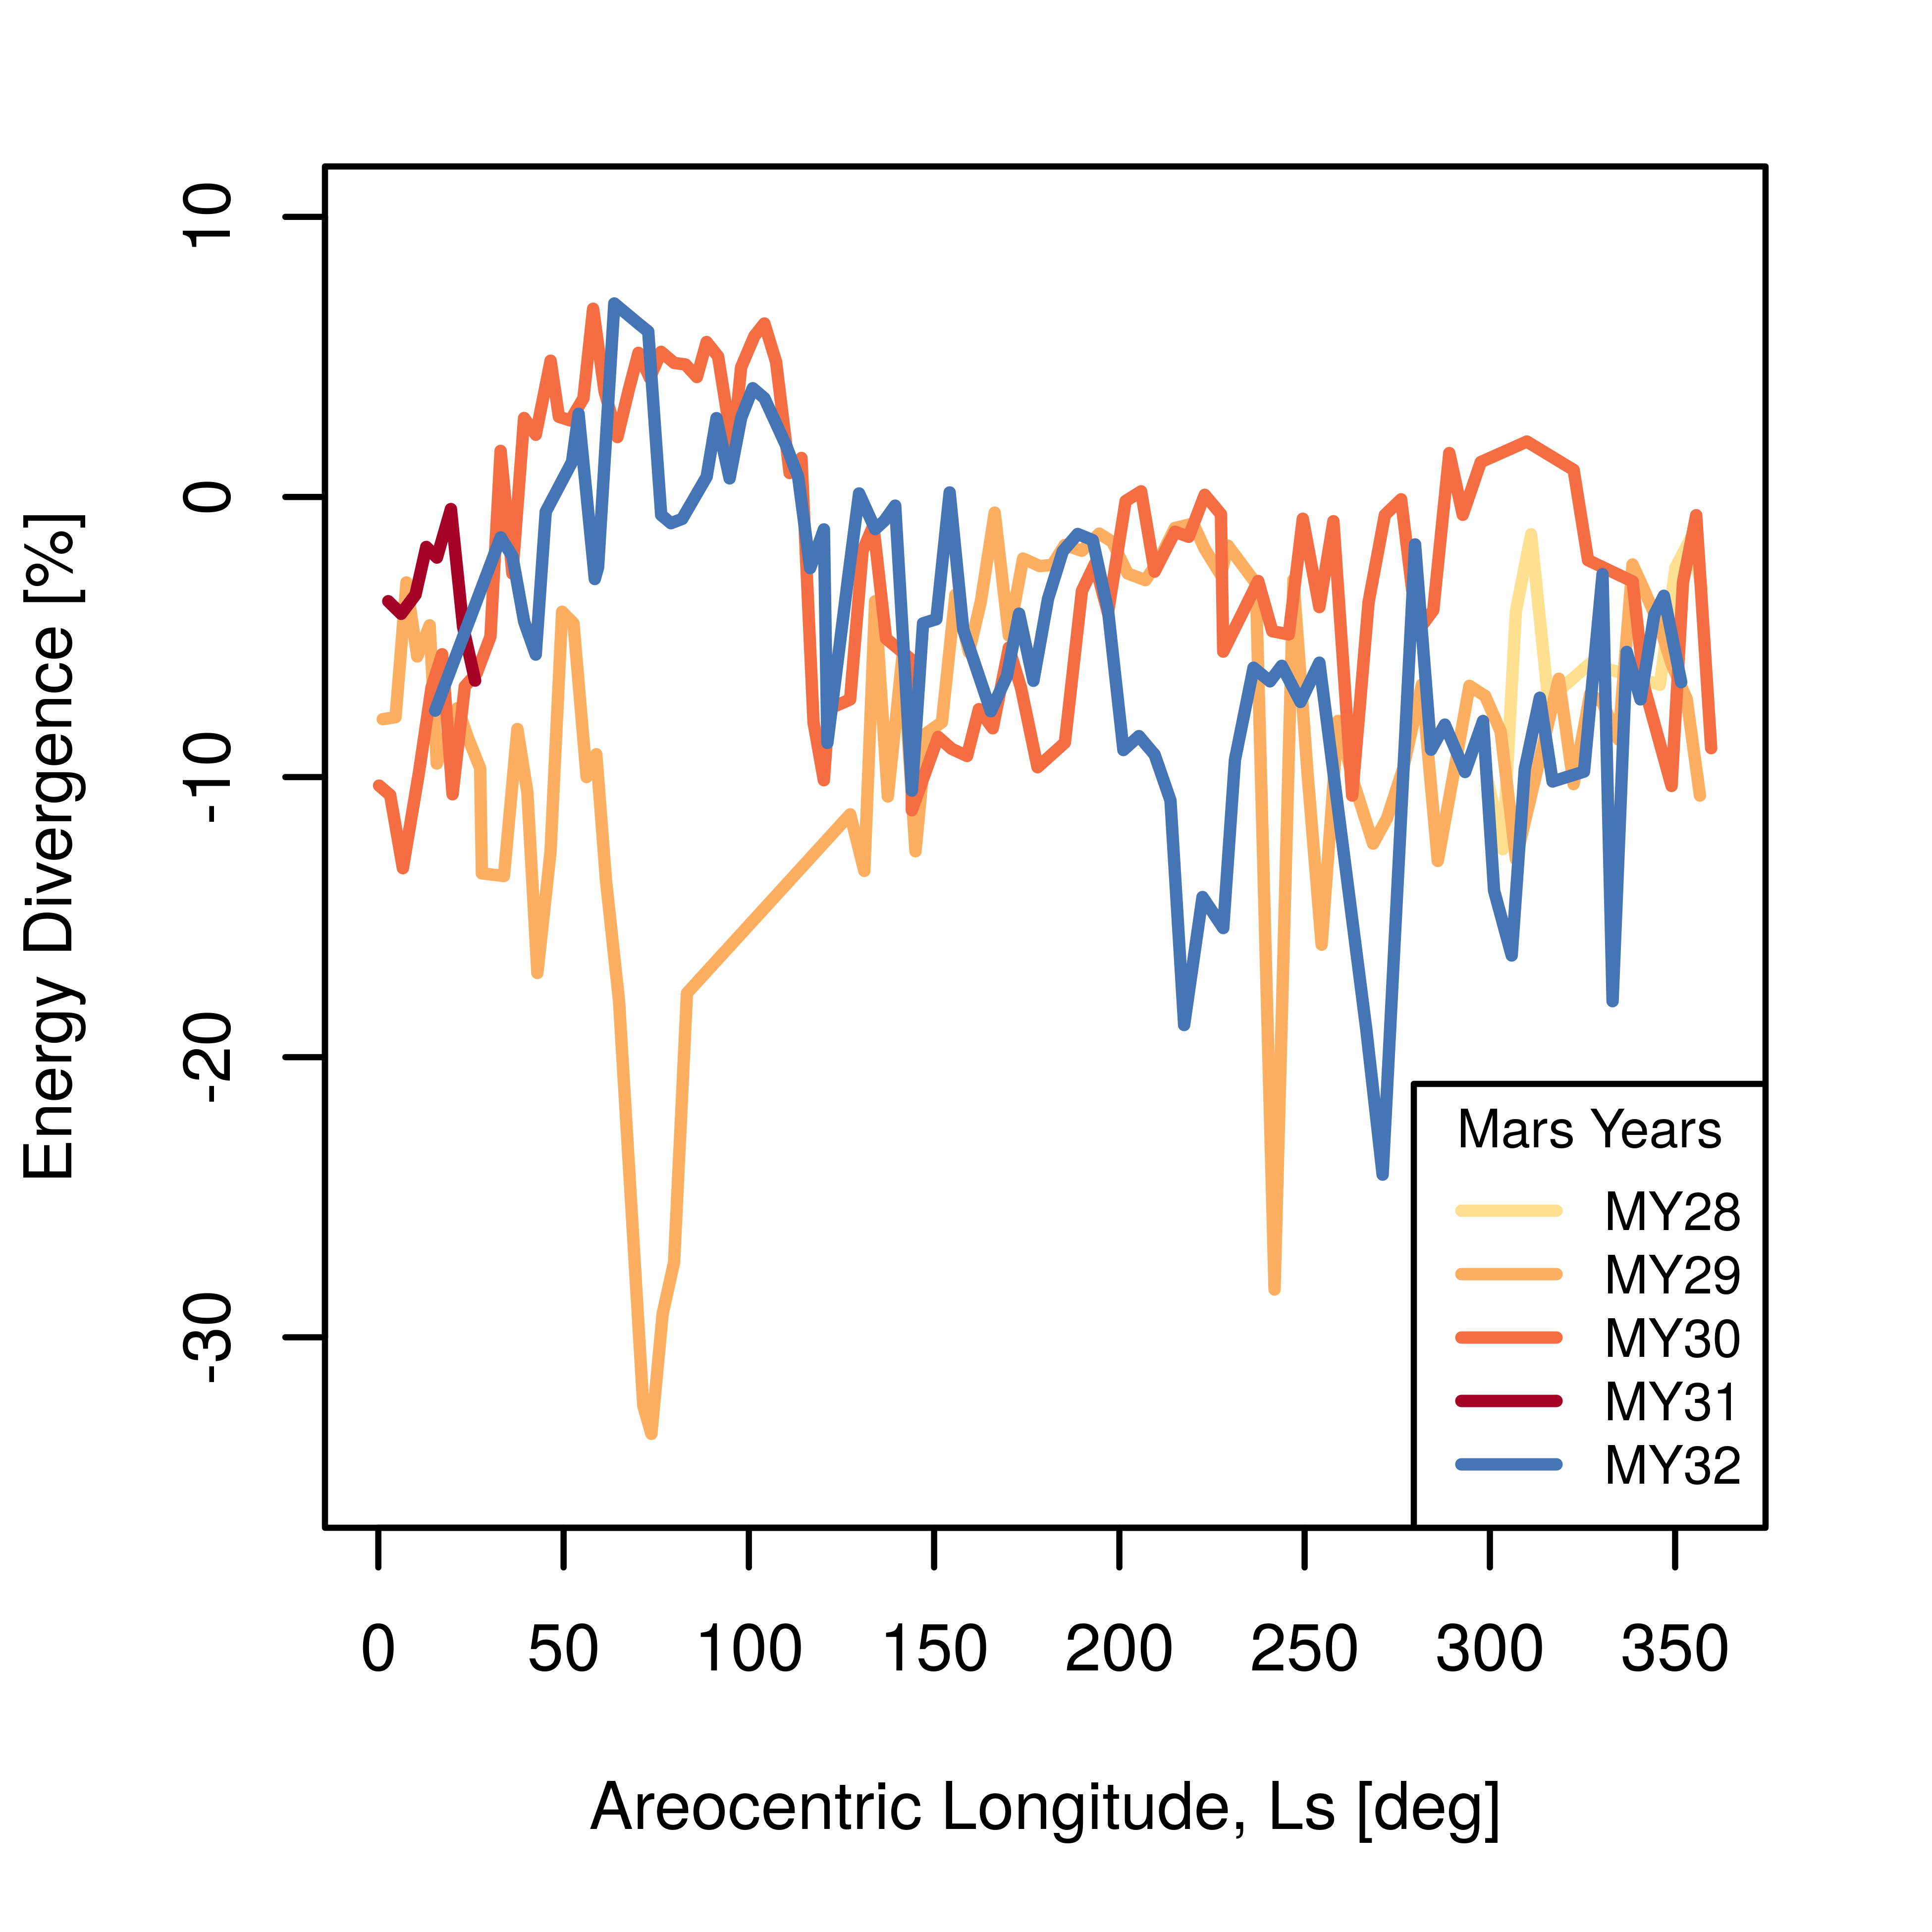
\includegraphics[width=0.8\linewidth]{sections/power-and-energy-predictions/plots/energy-prediction-divergences-from-my28-to-my32.png}\\
  \caption[Divergences from predicted \ac{MER} Opportunity \ac{PV} energy production]
          {Divergences from predicted \ac{MER} Opportunity \ac{PV} energy production.}
  \label{fig:plot:mer-energy-prediction-divergences}
\end{figure}

\clearpage

Figure \ref{fig:plot:binned-error-margins} bins the distribution of divergences across the -33\%/+7\% error margin range into 5\% increments. 65.5\% of the divergences occur within a -10\%/0\% error margin and 90.7\%  within -15\%/+5\%.

\begin{figure}[h]
  \centering
  \hypersetup{linkcolor=captionTextColor}
  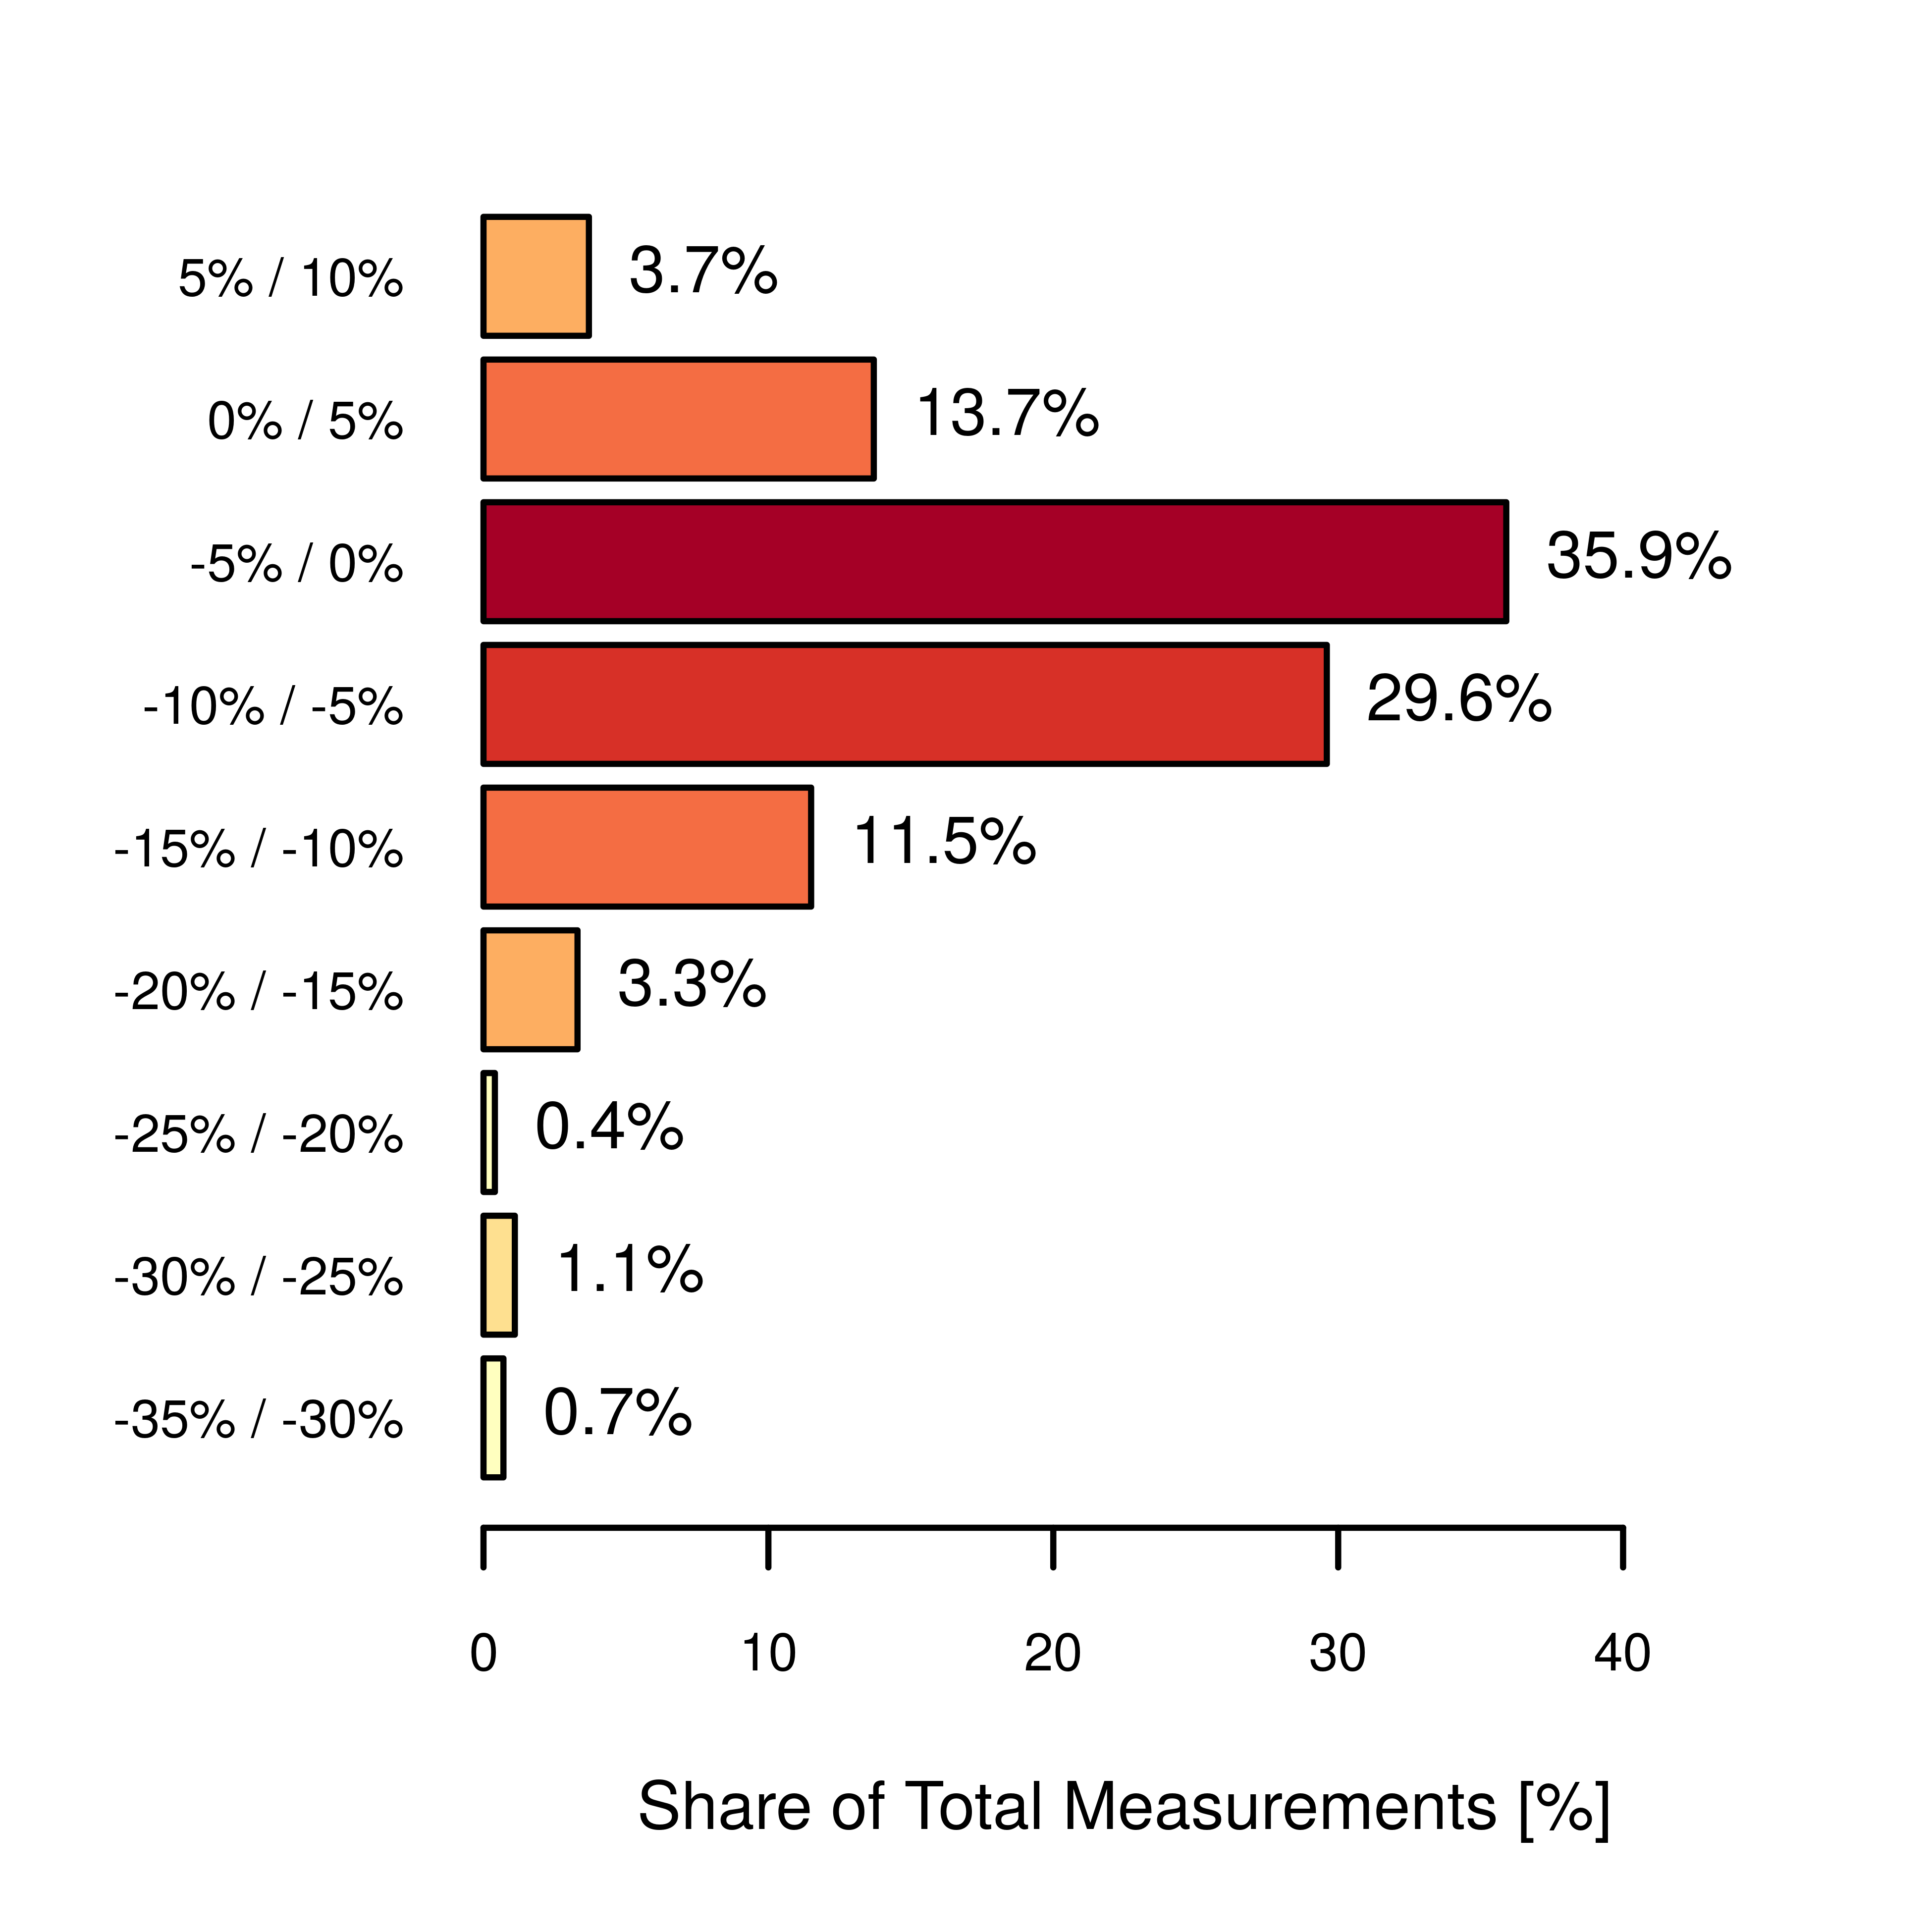
\includegraphics[width=0.8\linewidth]{sections/power-and-energy-predictions/plots/binned-error-margins.png}\\
  \caption[Binned error margins]
          {Binned error margins.}
  \label{fig:plot:binned-error-margins}
\end{figure}

The wide error margin range is thus a result of isolated local maxima outliers, notably at Sol 2204 (-33\%), 2218 (-27\%), 2519 (-28\%), and 3901 (-24\%). Table \ref{tab:divergences-less-than-m20pc} lists all divergences that are beyond -20\%.

\begin{table}[h]
    \centering
    \caption{Divergences from predicted MER Opportunity PV energy production that are beyond -20\%.}
    \label{tab:divergences-less-than-m20pc}
    \begin{tabular}{|l|c|c|c|c|c|c|c|}
    \hline
    \multicolumn{1}{|c|}{\multirow{2}{*}{\textbf{Date}}} & \multirow{2}{*}{\textbf{MY}} & \multirow{2}{*}{\textbf{Ls}} & \multirow{2}{*}{\textbf{Sol}} & \multicolumn{4}{c|}{\textbf{Energy [Wh]}} \\ \cline{5-8}
    \multicolumn{1}{|c|}{} &  &  &  & \textbf{Predicted} & \textbf{Measured} & \textbf{Diff.} & \textbf{Diff. [\%]} \\ \hline
    1-APR-2010 & 29 & 72 & 2199 & 315 & 238 & 77 & -32 \\
    6-APR-2010 & 29 & 74 & 2204 & 314 & 235 & 79 & -33 \\
    13-APR-2010 & 29 & 77 & 2211 & 293 & 227 & 66 & -29 \\
    20-APR-2010 & 29 & 80 & 2218 & 314 & 247 & 67 & -27 \\ \hline
    23-FEB-2011 & 29 & 242 & 2519 & 539 & 420 & 119 & -28 \\ \hline
    13-JAN-2015 & 32 & 271 & 3901 & 491 & 395 & 96 & -24 \\ \hline
    \end{tabular}
\end{table}


With the exception of Sol 2199 and 2218, possible explanations for large divergences beyond -20\% were obtained from MER Opportunity's status logs [?]:
\begin{enumerate}[(a)]
  \item Sol 2199: No turns or inclinations reported.
  \item Sol 2204: Turn - short sharp arc turn.
  \item Sol 2211: Inclination - crossed a series of ripples.
  \item Sol 2218: No turns or inclinations reported.
  \item Sol 2519: Turn - sharp repositioning turn.
  \item Sol 3901: Inclination - descended from the summit of 'Cape Tribulation'.
\end{enumerate}

\todo[inline]{TODO: Source MER Opportunity status log.}
%Sources. For terrestrial year 2010: https://mars.nasa.gov/mer/mission/rover-status/opportunity/2010/

The use of fixed daily values for the certain irradiance calculation variables also contributes to the observed divergences:
\begin{enumerate}[(a)]
  \item A fixed $\tau$ factor does not reflect the continuous changes in atmopheric optical depth.
  \item A fixed solar array dust factor does not reflect the irregularity of dust deposition over the entirety of the solar cell coverage area.
  \item A fixed shadowing performance loss coefficient does not reflect the diurnal changes in overshadowed area. Overshadowing changes throughout the day due to the position of the sun with respect to the location of the rover's petruding instruments, notably the Pancam Mast Assembly (PMA) as well as the low-gain and high-gain antennas.
\end{enumerate}

Attempts to narrow down the error margin range by adjusting the reported dust factor as well as shadowing and other losses are described in Appendix \ref{sec:Appendix:NarrowedEnergyPredictionErrorMarginRange}. However, these attempts resulted in overly conservative energy predictions and will not be applied.

By setting aside outliers causing divergences greater than 5\% and lesser than -15\% that were obtained with only 9.2\% of the dataset, the predicted energy production obtained with Equation \ref{eq:SA_energy} become acceptable for preliminary mission scenario analysis on a horizontal surfaces.

\clearpage
\subsection{Inclined Surface}
\label{sec:PowerAndEnergyPredictions:Validation:InclinedSurface}

Equation \ref{eq:SA_slope_energy} for energy predictions on an inclined surface requires slope and rover orientation angles in order to determine $H_{\beta}$. However, these parameters are seldom reported in the \ac{MER} Opportunity status updates.

Cherry-picked energy production measurements made while \ac{MER} Opportunity's descended into and ascended out of Endaveaour crater during MY33 were used in an attempt to validate predictions made with Equation \ref{eq:SA_slope_energy}. These measurements were selected based on traverse phases that preserved consistent orientations which could be more reliable measured from the rover's Traverse Map Archive [z].

An average slope angle of 13 degrees was assumed based on the following:
\begin{itemize}
  \item On Sol 4269 and 4270, \ac{MER} Opportunity status logs reported that the rover climbed slopes close to \SI{30}{\degree} near the crest of ``Knudsen Ridge'' [a], reaching \SI{32}{\degree} on March 10, 2016 (Sol 4310) [b].
  \item An image taken in March 22, 2016 (Sol 4322), was rotated \SI{13.5}{\degree} degrees to adjust for the tilt of the rover.
  \item Perseverance Valley extends downhill at around \SI{15}{\degree} for about 200 meters toward Endeavour crater's interior [c].
\end{itemize}

As was the case in Section \ref{sec:PowerAndEnergyPredictions:Validation:HorizontalSurface}, performance ratios described in Section \ref{sec:PowerAndEnergyPredictions:PerformanceRatio} were also used. Due to large uncertainties regarding slope rover orientation angles, this section only aims to validate that using Equation \ref{eq:SA_slope_energy} results in smaller energy predictions divergences than what would otherwise be obtained using Equation \ref{eq:SA_energy}. The results are presented in Table \ref{tab:divergences-inclined-surfaces}:

\begin{table}[h]
\centering
\caption{Divergences from predicted MER Opportunity PV energy production on inclined surfaces.}
\label{tab:divergences-inclined-surfaces}
\begin{tabular}{|c|c|c|c|c|c|}
\hline
\multicolumn{1}{|l|}{\multirow{3}{*}{\textbf{Sol}}} & \multirow{3}{*}{\textbf{\begin{tabular}[c]{@{}c@{}}Measured\\ Energy\\ {[}Wh{]}\end{tabular}}} & \multicolumn{4}{c|}{\textbf{Predicted Energy}} \\ \cline{3-6}
\multicolumn{1}{|l|}{} &  & \multicolumn{2}{c|}{\textbf{Horizontal Surface}} & \multicolumn{2}{c|}{\textbf{Inclined Surface}} \\ \cline{3-6}
\multicolumn{1}{|l|}{} &  & \multicolumn{1}{l|}{\textbf{$E$ {[}Wh{]}}} & \multicolumn{1}{l|}{\textbf{Diff. {[}\%{]}}} & \multicolumn{1}{l|}{\textbf{$E_{\beta}$ {[}Wh{]}}} & \multicolumn{1}{l|}{\textbf{Diff. {[}\%{]}}} \\ \hline
4493 & 515 & 653 & -27 & 407 & 21 \\ \hline
4582 & 411 & 595 & -45 & 535 & -30 \\ \hline
4623 & 416 & 583 & -40 & 284 & 32 \\ \hline
4630 & 466 & 595 & -28 & 526 & 13 \\ \hline
\end{tabular}
\end{table}


Equation \ref{eq:SA_slope_energy} resulted in a larger divergence range than with Equation \ref{eq:SA_energy} at -30\%/32\% for the former and -45\%/-27\% for the latter. However, the magnitude of divergences are smaller with Equation \ref{eq:SA_slope_energy}. Furthermore, with the exception of Sol 4582, divergences with \ref{eq:SA_slope_energy} result in conservative under-estimated energy predictions rather than the worst-case over-estimated values consistently obtained with Equation \ref{eq:SA_energy}.

The pool of measured data used for this validation was much too small to draw convincing conclusions and the magnitude of divergences remained significantly large. Inaccurate slope and rover orientation angles are likely to have contributed to unfavourable results. Further data will have to be obtained to validate Equation \ref{eq:SA_slope_energy} against reported measurements. However, for the purpose of this thesis, mission scenario analysis on inclined surfaces will still rely on predictions obtained with Equation \ref{eq:SA_slope_energy} in light of it being derived from applying solar geometry to Equation \ref{eq:SA_energy}, with which favourably results were obtained as described in Section \ref{sec:PowerAndEnergyPredictions:Validation:HorizontalSurface}.

% [z] Rover traverse map. [https://mars.nasa.gov/mer/mission/traverse-maps/opportunity/]
% [a] https://mars.nasa.gov/mer/mission/rover-status/opportunity/recent/all/?y=2016
% [b] https://www.jpl.nasa.gov/news/news.php?feature=6193
% [c] https://www.planetary.org/explore/space-topics/space-missions/mer-updates/2018/04-mer-update-special-perseverance-valley-lpsc-2018.html

%Particularly while it was exploring steep outcrops within 'Marathon Valley' when the rover was inclined on the slopes of 'Knudsen Ridge' at Sol 4303 (March 1, 2016).
%The rover's tilt hit 32 degrees on March 10 while Opportunity was making its closest approach to an intended target near the crest of "Knudsen Ridge."

%%%%%%%%%%%%%%%%%%%%%%%%%%%%%%%%%%%%%%%%%%%%%%%%%%%%%%%


%%%%%%%%%%%%%%%%%%%%%%%%%%%%%%%%%%%%%%%%%%%%%%%%%%%%%%%
\chapter{Requirements and Design Drivers}
%\shinyChapterQuote{Adjusting to the requirement for perfection is, I think, the most difficult part of learning to program.}
%  {Frederick P. Brooks Jr., The Mythical Man-Month: Essays on Software Engineering}
% Also: For the human makers of things, the incompletenesses and inconsistencies of our ideas become clear only during implementation.
\label{sec:RequirementsAndDesignDrivers}
%%%%%%%%%%%%%%%%%%%%%%%%%%%%%%%%%%%%%%%%%%%%%%%%%%%%%%%


%%%%%%%%%%%%%%%%%%%%%%%%%%%%%%%%%%%%%%%%%%%%%%%%%%%%%%%
\chapter{Solar Array Design, Integration, and Deployment Mechanism}
%\shinyChapterQuote{Mechanisms and mechanical systems, everybody can design them but everybody has a hard time making them work.}
%  {Aaron Cohen, Engineering the Space Shuttle.}
\label{sec:SolarArrayDesign}
%%%%%%%%%%%%%%%%%%%%%%%%%%%%%%%%%%%%%%%%%%%%%%%%%%%%%%%


%%%%%%%%%%%%%%%%%%%%%%%%%%%%%%%%%%%%%%%%%%%%%%%%%%%%%%%
\chapter{Battery Configuration}
%\shinyChapterQuote{}
\label{sec:BatteryConfiguration}
%%%%%%%%%%%%%%%%%%%%%%%%%%%%%%%%%%%%%%%%%%%%%%%%%%%%%%%


%%%%%%%%%%%%%%%%%%%%%%%%%%%%%%%%%%%%%%%%%%%%%%%%%%%%%%%
\chapter{Mission Scenarios}
%\shinyChapterQuote{Maybe I’ll post a consumer review. “Brought product to surface of Mars. It stopped working. 0/10.”}
%  {Andy Weir, The Martian.}
\label{sec:MissionScenarios}
%%%%%%%%%%%%%%%%%%%%%%%%%%%%%%%%%%%%%%%%%%%%%%%%%%%%%%%


%%%%%%%%%%%%%%%%%%%%%%%%%%%%%%%%%%%%%%%%%%%%%%%%%%%%%%%
\chapter{Conclusion and Outlook}
%\shinyChapterQuote{}
\label{sec:ConclusionAndOutlook}
%%%%%%%%%%%%%%%%%%%%%%%%%%%%%%%%%%%%%%%%%%%%%%%%%%%%%%%

%%%%%%%%%%%%%%%%%%%%%%%%%%%%%%%%%%%%%%%%%%%%%%%%%%%%%%
%#%\chapter[Requirements and Design Drivers: Heterogeneous Modular Multi-Robot Systems] %%for toc
%#%        [Design Drivers: Heterogeneous Modular Multi-Robot Systems] %% for head
%#%        {Requirements and Design Drivers: Heterogeneous Modular \\ Multi-Robot Systems} %%for chapter page
%#%\label{sec:ReqirementsConditions}
%#%\shinyChapterQuote{A shiny quote for the start?}
%#%       {If you like to.}
%#%This is an example chapter for usage of three types of chapter headings. (see source file)
%\acresetall                 %% reset all acronym abbreviations and write first appearance long
%\acused{CAD}
\acused{DoF}
\acused{EEPROM}
\acused{FPGA}
\acused{GPS}
\acused{HD}
\acused{LED} %%define ackronyms that are "common sense"

%%%%%%%%%%%%%%%%%%%%%%%%%%%%%%%%%%%%%%%%%%%%%%%%%%%%%%



%%%%%%%%%%%%%%%%%%%%%%%%%%%%%%%%%%%%%%%%%%%%%%%%%%%%%%
%#%\chapter{\ElecMech Rover Design}
%#%\label{sec:RobotDesign}
%\acresetall                 %% reset all acronym abbreviations and write first appearance long
%\acused{CAD}
\acused{DoF}
\acused{EEPROM}
\acused{FPGA}
\acused{GPS}
\acused{HD}
\acused{LED} %%define ackronyms that are "common sense"
%#%
%%-----------------------------------------------
\shinyChapterQuote{[...] development of robotic mechanization and control architectures that enable roving into
adverse, challenging terrain -- areas that can change dramatically over short distances -- is of considerable importance.}
{\citesota{Schenker2001}}


%%-----------------------------------------------
This chapter ... \todo{what is to be expected of this chapter?}

%%-----------------------------------------------
%\chapterSupportedBy{\designCites}
%\designCites
%\todo{check long list vs. short list macros!}
\chapterSupportedBy{\designCitesLong}



%%-----------------------------------------------

\section{Design Considerations}
\label{sec:design:considerations}
\lipsum


\section{System Design: Mechanics}
\label{sec:design:mechanics}
\input{sections/RobotDesign_mechanics.tex}


\section{Summary and Conclusion}
\label{sec:design:SummaryConclusion}
\todo[inline]{Always a good idea to give a short conclusion per chapter}



%%%%%%%%%%%%%%%%%%%%%%%%%%%%%%%%%%%%%%%%%%%%%%%%%%%%%%



%%%%%%%%%%%%%%%%%%%%%%%%%%%%%%%%%%%%%%%%%%%%%%%%%%%%%%
%#%\chapter{Control System Design}
%#%\label{sec:control}
%\acresetall                 %% reset all acronym abbreviations and write first appearance long
%\acused{CAD}
\acused{DoF}
\acused{EEPROM}
\acused{FPGA}
\acused{GPS}
\acused{HD}
\acused{LED} %%define ackronyms that are "common sense"
%#%%%-----------------------------------------------
\shinyChapterQuote{If everything seems under control, \newline
       you're just not going fast enough.}
       {Mario Andretti}
%%-----------------------------------------------

This chapter \todo{...shows what?}

%%-----------------------------------------------
%\chapterSupportedBy{\mcsCites}
%\mcsCites
%\todo{check long list vs. short list macros!}
\chapterSupportedBy{\controlCitesLong}

%%-----------------------------------------------




%\begin{itemize}
%%   \setlength\itemsep{0em}
%%   \setlength\topsep{0em}
%  \item reactive control and advantages for planetary rovers, p2/14
%  \item layers of control... HL, MW, LL
%  \item
%\end{itemize}


\section{A}
\label{sec:control:Structure}
%\input{sections/ControlSystemDesign_.tex}
\lipsum


\section{Coordinate Systems for Locomotion Control}
\label{sec:control:kinematicsConsiderations}
%\input{sections/ControlSystemDesign_.tex}


\section{Summary and Conclusion}
\label{sec:control:Conclusion}
This chapter presents ....

\lipsum






%%%%%%%%%%%%%%%%%%%%%%%%%%%%%%%%%%%%%%%%%%%%%%%%%%%%%%



%%%%%%%%%%%%%%%%%%%%%%%%%%%%%%%%%%%%%%%%%%%%%%%%%%%%%%
%#%\chapter{Experimental Evaluation}
%#%\label{sec:Experiments}
%\acresetall                 %% reset all acronym abbreviations and write first appearance long
%\acused{CAD}
\acused{DoF}
\acused{EEPROM}
\acused{FPGA}
\acused{GPS}
\acused{HD}
\acused{LED} %%define ackronyms that are "common sense"
%#%%%-----------------------------------------------
\shinyChapterQuote{No amount of experimentation can ever prove me right; \newline
       a single experiment can prove me wrong.}
       {Albert Einstein}


%%-----------------------------------------------


This chapter of the thesis summarizes the experiments and results conducted for ... \todo{!}


%%-----------------------------------------------
%\chapterSupportedBy{\expCites}
%\expCites
%\todo{check long list vs. short list macros!}
\chapterSupportedBy{\expCitesLong}

%%-----------------------------------------------

\section{General Experimental Setup and Evaluation Methods}
\label{sec:Experimente:Setup}
%\input{sections/experiments_setup.tex}


\section{Experiment 1}
\label{sec:Experiments:Exp1}
%\input{sections/experiments_1.tex}

\section{Experiment 2}
\label{sec:Experiments:Exp2}
%\input{sections/experiments_2.tex}


\section{Summary and Conclusion} 
\label{sec:Experiments:Conclusion}
This chapter presents the \electromech system design of the two rover versions Sherpa and SherpaTT.
General design decisions valid for both systems are presented with the main influences resulting from the respective \ac{MRS}.
Apart from the kinematic design of the suspension systems, the central power management is discussed as this is a central part for the rovers to be a fully functional subsystem of a modular \ac{MRS}.

A manipulation arm for both rovers is developed using an evolutionary algorithm for morphology optimization.
Several use-cases are defined and a trajectory for the arm is built to test the use-cases in a physical simulation for fitness evaluation of the respective individuum.
The arm is then manufactured following a biologically inspired manufacturing methodology.
%Both rover systems make use of the same manipulation arm.

Comparing the main features of both implemented rover systems shows basically the same leg length of the first and second suspension generation, \refTab{tab:Design:ComparisonSherpaSherpaTT}.
The mass per leg as well as the total system mass are nearly identical as well.
With five \ac{DoF} per leg, the second generation suspension has one \ac{DoF} less per leg.
Horizontal and vertical \ac{LEP} movements in Sherpa are coupled, while they are independent in SherpaTT.
Note that the vertical and horizontal stroke listed for SherpaTT in the table are those resulting from the currently set software-joint limits as also shown in \refFig{fig:SherpaTT_Workspace-2d}.
Exploiting the full mechanical range as provided in \refTab{tab:AntriebsdatenSherpaTT} results in 860\unitmm vertical and 629\unitmm horizontal stroke.

\begin{table}[h]
%\vspace{-2ex}
  %\centering
  \hypersetup{hidelinks=true}
  %
  \caption[Comparison of main features of suspension system generations and rovers]{Comparison of main features of suspension system generations and rovers.
  %\dissExtraCaption{The stow footprint is measured using the \acp{LEP}, while the stow volume is a cuboid enclosing all parts of the rover, including those overhanging the \ac{LEP}'s footprint.}
  }
  \label{tab:Design:ComparisonSherpaSherpaTT}
  \begin{footnotesize}
      \begin{tabular}{l| rrr r ll r rr}
        \toprule
         \rowcolor{tableheadingcolor}
        System  & Leg length & Mass    & Mass & \ac{DoF}         & vert. & horz. & min stow  & \multicolumn{2}{c}{compactness}\\
        \rowcolor{tableheadingcolor}
                & zero pose &  (leg)  & total  & (leg)   & stroke &  stroke &volume    & footprint & volume \\
        \midrule
        \cellcolor{tablesubheadingcolor}Sherpa      & 976\unitmm & 25\unitkg & 160\unitkg &6          & 900\unitmm
%        \color{captionTextColor}{$^{\ast}$}
        & 260\unitmm
%        \color{captionTextColor}{$^{\ast\ast}$}
        &  2.24\unitcubmeter & 0.40 & 0.64\\
        \cellcolor{tablesubheadingcolor}SherpaTT\hspace{-1mm}    & 977\unitmm & 26\unitkg & \massSherpaTT &5          & 775\unitmm & 485\unitmm & 1.67\unitcubmeter & 0.79 & 0.72\\
        \bottomrule
      \end{tabular}
  \end{footnotesize}
  %\begin{scriptsize}
       % \vspace{-2mm}
%        \begin{flushleft}
%            \color{captionTextColor}{
%                $^{\ast}$ ~~~only possible with simultaneously changing horizontal position
%            \newline
%                $^{\ast\ast}$ ~\,only possible with simultaneously changing vertical position
%            %\newline
%%                $^{\ast\ast\ast}$ software safety limitation of IL and OL actuators, full range with mechanical limits: 860\unitmm and 629\unitmm see \refTab{tab:AntriebsdatenSherpaTT}.
%            }
%    \end{flushleft}
%    \end{scriptsize}
    %\vspace{-3ex}
\end{table}

Due to improved arrangement of the \ac{DoF}, the minimum stow volume is reduced from 2.24\unitcubmeter to 1.67\unitcubmeter.
This is also reflected in the values of compactness provided in the table; these values are based on the isoperimetric quotient:
The ratio of the area of the footprint to the area of a circle with the same perimeter is built.
A circle is the most compact shape in two-dimensional space,
therefore, the ratio ranges between 0 and 1 with high compactness being close to 1.
Similarly the compactness of the three-dimensional envelope volume is calculated using a sphere as most compact volume.
In both cases, the new design achieves higher compactness values.
%Higher compactness bears the potential for better fitting into a lander structure for transfer to Moon or Mars.



Apart from the compactness, the new arrangement of the \ac{DoF} allows to place the \ac{LEP} in a three-dimensional workspace compared to a two-dimensional spherical surface.
This design generates internal mobilities, that can be used to facilitate deployment and pickup of immobile elements in the \ac{MRS}.
Furthermore, the position and orientation of the central body in the support polygon can be changed without moving the wheels over the ground, which is beneficial for \ac{CoG} relocations in intricate slopes with low traction surface material.

A six \ac{DoF} \ac{FTS} is present in each leg of the new suspension system design.
Direct ground contact force measurement becomes available with this sensor, which in turn allows improved load balancing between the rover's ground contact points.

To conclude, with basically the same dimensioning (size, weight), superior properties are presented with the second suspension system design.
The subsequent chapters focus on the control and evaluation of this new suspension system and the rover SherpaTT.





%%%%%%%%%%%%%%%%%%%%%%%%%%%%%%%%%%%%%%%%%%%%%%%%%%%%%%



%%%%%%%%%%%%%%%%%%%%%%%%%%%%%%%%%%%%%%%%%%%%%%%%%%%%%%
%#%\chapter{Conclusion and Outlook}
%#%\label{sec:ConclusionOutlook}
%#%\todo[inline]{The very important findings of this thesis go here}
%%%%%%%%%%%%%%%%%%%%%%%%%%%%%%%%%%%%%%%%%%%%%%%%%%%%%%


%% redefine headers for Bibliography
\makeevenhead{ruled}{\itshape\leftmark}{}{}
\makeoddhead{ruled}{}{}{\itshape\rightmark}
\pagestyle{ruled}

\addTocCaption{Bibliography}

\begin{small}
%\addcontentsline{toc}{chapter}{Bibliography}
%\bibliographystyle{alpha}
%\bibliography{../../ownPublications} % literaturverzeichnis
\bibliographymarsenv{references/marsenv}
\bibliographypower{references/power}
\bibliographyother{references/other}
\end{small}
\cleardoublepage


%#%\todo[inline]{check printing/digital flag for link colors}


%% redefine headers for Appendix
\makeevenhead{ruled}{\scshape Appendix \leftmark}{}{}
\makeoddhead{ruled}{}{}{\itshape\rightmark}
\pagestyle{ruled}

\begin{appendix}

\end{appendix}\addTocCaption{Appendix}
%\addcontentsline{toc}{chapter}{Appendix}
%\backmatter %%changes formatting!

\chapter{Insolation Calculation Verification}
\label{sec:Appendix:InsolationCalculationVerification}
The formulae for insolation calculations were taken from \citemarsenv{Appelbaum1989}, \citemarsenv{Appelbaum1990}, \citemarsenv{Appelbaum1991}, and \citemarsenv{Appelbaum1993}. For the purpose of this thesis, the formulae were implemented into an R package to be used in mission analysis power budgets and energy predictions. Both \citemarsenv{Appelbaum1990} and \citemarsenv{Appelbaum1993} include tables listing pre-calculated insolation values for horizontal and inclined surfacesnat \ac{VL1} and \ac{VL2} locations. These published values were used to validate the R implementation of the insolation formulae. This chapter compares the published and calculated insolation values with each other in order to verify and validate the R package derived from publication.


\section{Horizontal Surface}
\lipsum 
\clearpage

\section{Inclined Surface with Beta Equals Phi}
\subsection{At Viking Lander 1 (VL1)}
Figure \ref{fig:sub:comparative-global-insolation-at-vl1-beta-equals-phi-daily-variations} shows that calculated values are consistently lower than those published in \citemarsenv{Appelbaum1993}. Both daily variations closely follow the same pattern. Figure \ref{fig:sub:comparative-global-insolation-at-vl1-beta-equals-phi-percentage-differences} reveals that the differences between calculated and published values range between \SI{2.1}{\percent} and \SI{3.1}{\percent}. Differences larger than \SI{2.5}{\percent} are more frequent for small tau values, particularly below 1.

\begin{figure}[H]
\captionsetup[subfigure]{justification=centering}
\vspace{-2ex}
\centering
    %% setup sizes
    \setlength{\subfigureWidth}{0.50\textwidth}
    \setlength{\graphicsHeight}{80mm}
    %% kill hyper-link highlighting
    \hypersetup{hidelinks=true}%
    %% the figures
    \begin{subfigure}[t]{\subfigureWidth}
        \centering
            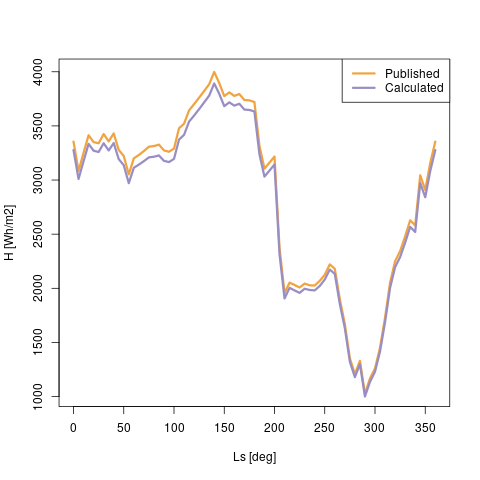
\includegraphics[height=\graphicsHeight]{sections/appendix/A/plots/h-exp-calc-at-vl1-with-beta-223-deg.png}
            \subcaption{Daily variations.}
            \label{fig:sub:comparative-global-insolation-at-vl1-beta-equals-phi-daily-variations}
    \end{subfigure}\hfill
    \begin{subfigure}[t]{\subfigureWidth}
        \centering
            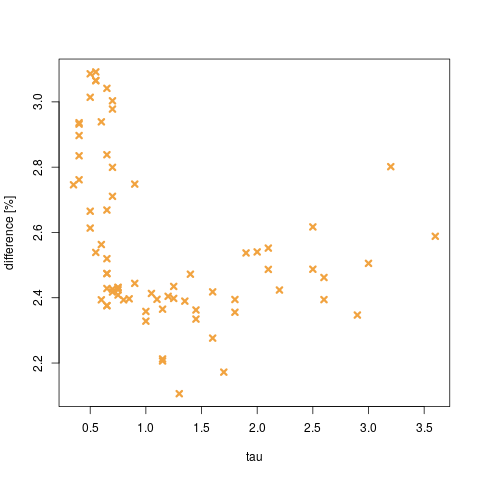
\includegraphics[height=\graphicsHeight]{sections/appendix/A/plots/h-diff-bet-exp-calc-at-vl1-with-beta-223-deg.png}
            \subcaption{Differences as a function of optical depth.}
            \label{fig:sub:comparative-global-insolation-at-vl1-beta-equals-phi-percentage-differences}
    \end{subfigure}\\[0.8ex]
    \caption{Comparison between published and calculated daily global insolations at \ac{VL1} on a inclined surface with $\beta=\SI{22.3}{\degree}$.}
    \label{fig:plot:comparative-global-insolation-at-vl1-beta-equals-phi}
\vspace{-2ex}
\end{figure}

\subsection{At Viking Lander 2 (VL2)}
Figure \ref{fig:sub:comparative-global-insolation-at-vl2-beta-equals-phi-daily-variations} shows that calculated values are consistently lower than those published in \citemarsenv{Appelbaum1993}. Both daily variations closely follow the same patterns. Figure \ref{fig:sub:comparative-global-insolation-at-vl2-beta-equals-phi-percentage-differences} reveals that the differences between calculated and published values range between \SI{0.4}{\percent} and \SI{6.6}{\percent}. Differences larger than \SI{3}{\percent} are more frequent for small tau values, particularly from 0.25 to 0.5 with differences larger than \SI{6}{\percent} for tau 0.4 and 0.5.

\begin{figure}[H]
\captionsetup[subfigure]{justification=centering}
\vspace{-2ex}
\centering
    %% setup sizes
    \setlength{\subfigureWidth}{0.50\textwidth}
    \setlength{\graphicsHeight}{80mm}
    %% kill hyper-link highlighting
    \hypersetup{hidelinks=true}%
    %% the figures
    \begin{subfigure}[t]{\subfigureWidth}
        \centering
            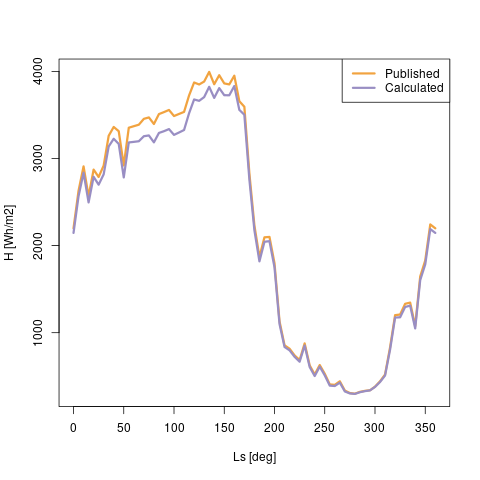
\includegraphics[height=\graphicsHeight]{sections/appendix/A/plots/h-exp-calc-at-vl2-with-beta-477-deg.png}
            \subcaption{Daily variations.}
            \label{fig:sub:comparative-global-insolation-at-vl2-beta-equals-phi-daily-variations}
    \end{subfigure}\hfill
    \begin{subfigure}[t]{\subfigureWidth}
        \centering
            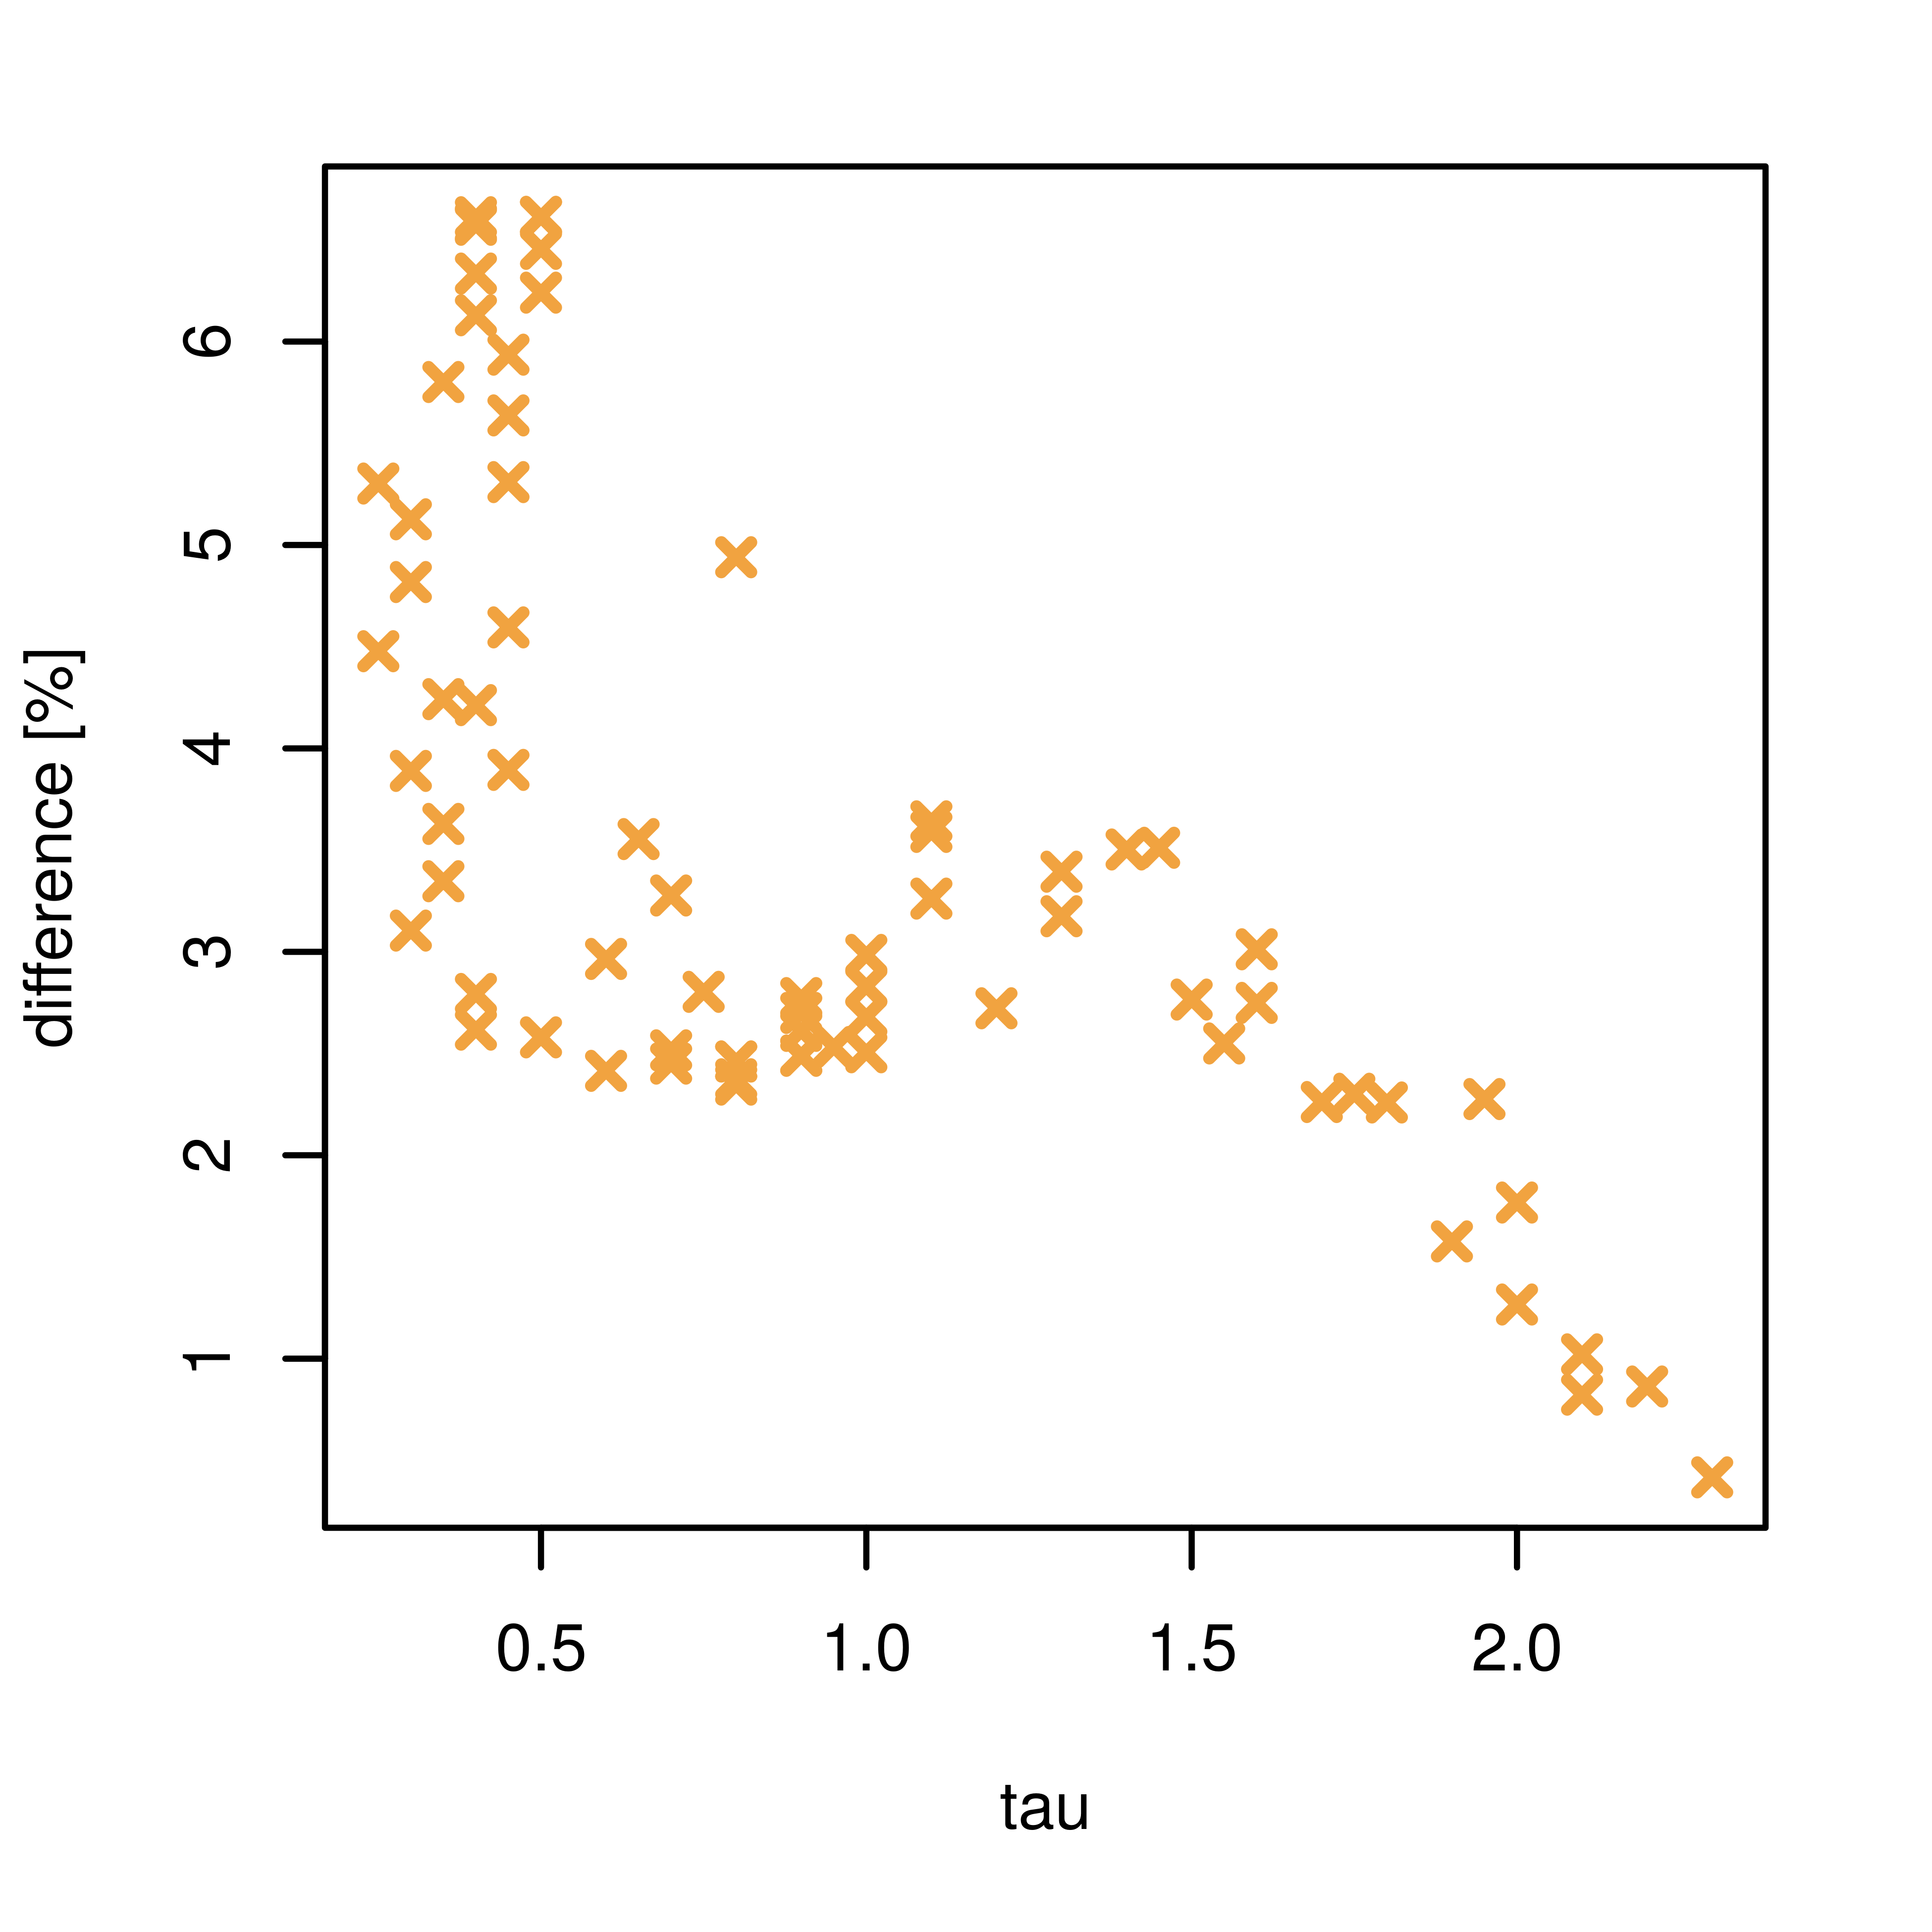
\includegraphics[height=\graphicsHeight]{sections/appendix/A/plots/h-diff-bet-exp-calc-at-vl2-with-beta-477-deg.png}
            \subcaption{Differences as a function of optical depth.}
            \label{fig:sub:comparative-global-insolation-at-vl2-beta-equals-phi-percentage-differences}
    \end{subfigure}\\[0.8ex]
    \caption{Comparison between published and calculated daily global insolations at \ac{VL2} on a inclined surface with $\beta=\SI{47.7}{\degree}$.}
    \label{fig:plot:comparative-global-insolation-at-vl2-beta-equals-phi}
\vspace{-2ex}
\end{figure}

\clearpage

\section{Inclined Surface with Optimal Beta Angle}
\subsection{At Viking Lander 1 (VL1)}
Figure \ref{fig:sub:comparative-global-insolation-at-vl1-beta-optimal-daily-variations} shows that calculated values are consistently lower than those published in \citemarsenv{Appelbaum1993}. Both daily variations closely follow the same pattern. Figure \ref{fig:sub:comparative-global-insolation-at-vl1-beta-optimal-percentage-differences} reveals that the differences between calculated and published values range between \SI{2}{\percent} and \SI{2.8}{\percent}. Differences larger than \SI{2.5}{\percent} are more frequent for large tau values starting from 1.9.

\begin{figure}[H]
\captionsetup[subfigure]{justification=centering}
\vspace{-2ex}
\centering
    %% setup sizes
    \setlength{\subfigureWidth}{0.50\textwidth}
    \setlength{\graphicsHeight}{80mm}
    %% kill hyper-link highlighting
    \hypersetup{hidelinks=true}%
    %% the figures
    \begin{subfigure}[t]{\subfigureWidth}
        \centering
            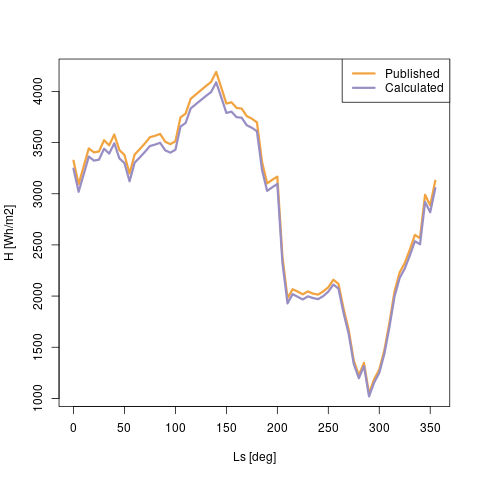
\includegraphics[height=\graphicsHeight]{sections/appendix/A/plots/h-exp-calc-at-vl1-with-beta-65-deg.png}
            \subcaption{Daily variations.}
            \label{fig:sub:comparative-global-insolation-at-vl1-beta-optimal-daily-variations}
    \end{subfigure}\hfill
    \begin{subfigure}[t]{\subfigureWidth}
        \centering
            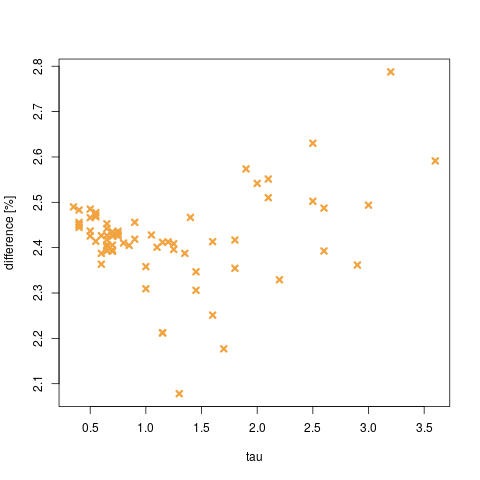
\includegraphics[height=\graphicsHeight]{sections/appendix/A/plots/h-diff-bet-exp-calc-at-vl1-with-beta-65-deg.png}
            \subcaption{Differences as a function of optical depth.}
            \label{fig:sub:comparative-global-insolation-at-vl1-beta-optimal-percentage-differences}
    \end{subfigure}\\[0.8ex]
    \caption{Comparison between published and calculated daily global insolations at \ac{VL1} on a inclined surface with $\beta=\SI{6.5}{\degree}$.}
    \label{fig:plot:comparative-global-insolation-at-vl1-beta-optimal}
\vspace{-2ex}
\end{figure}

\subsection{At Viking Lander 2 (VL2)}
Figure \ref{fig:sub:comparative-global-insolation-at-vl2-beta-optimal-daily-variations} shows that calculated values are consistently lower than those published in \citemarsenv{Appelbaum1993}. Both daily variations closely follow the same patterns. Figure \ref{fig:sub:comparative-global-insolation-at-vl2-beta-optimal-percentage-differences} reveals that the differences between calculated and published values range between \SI{0.4}{\percent} and \SI{3.7}{\percent}. Differences larger than \SI{2.5}{\percent} are more frequent for small tau values, particularly below 1.6.

\begin{figure}[H]
\captionsetup[subfigure]{justification=centering}
\vspace{-2ex}
\centering
    %% setup sizes
    \setlength{\subfigureWidth}{0.50\textwidth}
    \setlength{\graphicsHeight}{80mm}
    %% kill hyper-link highlighting
    \hypersetup{hidelinks=true}%
    %% the figures
    \begin{subfigure}[t]{\subfigureWidth}
        \centering
            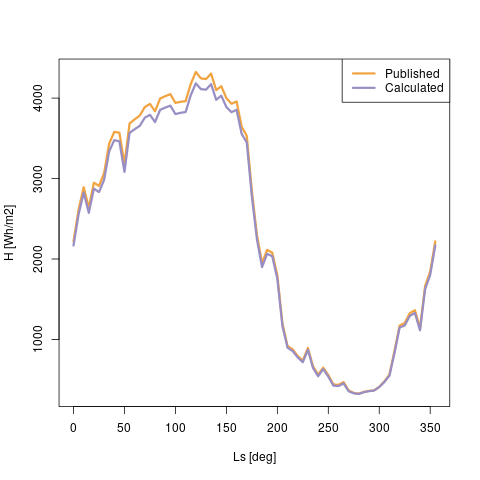
\includegraphics[height=\graphicsHeight]{sections/appendix/A/plots/h-exp-calc-at-vl2-with-beta-22-deg.png}
            \subcaption{Daily variations.}
            \label{fig:sub:comparative-global-insolation-at-vl2-beta-optimal-daily-variations}
    \end{subfigure}\hfill
    \begin{subfigure}[t]{\subfigureWidth}
        \centering
            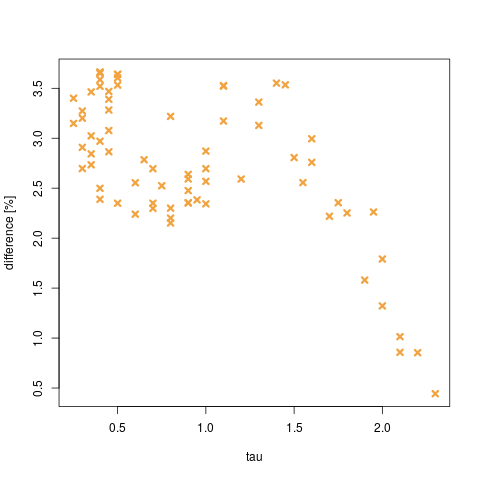
\includegraphics[height=\graphicsHeight]{sections/appendix/A/plots/h-diff-bet-exp-calc-at-vl2-with-beta-22-deg.png}
            \subcaption{Differences as a function of optical depth.}
            \label{fig:sub:comparative-global-insolation-at-vl2-beta-optimal-percentage-differences}
    \end{subfigure}\\[0.8ex]
    \caption{Comparison between published and calculated daily global insolations at \ac{VL2} on a inclined surface with $\beta=\SI{22}{\degree}$.}
    \label{fig:plot:comparative-global-insolation-at-vl2-beta-optimal}
\vspace{-2ex}
\end{figure}

\clearpage

\section{Conclusion}
It is not fully understood why differences exist between published and calculated global insolation values considering that, to the best of the author's knowledge, the same input parameters were used in both cases. Not presented in this chapter are differences for the beam, diffuse, and albedo components that compose the global insolation. These do not suggest that a single component is the source of the issue. Analyzing the differences as a function of tau hints that the issue is closely related to tau value inputs. Possible explanations could be:
\begin{itemize}
    \item The normalized net flux function lookup tables was used for insolations presented in \citemarsenv{Appelbaum1990} and \citemarsenv{Appelbaum1993} rather than approxmiated via the polynomial expression.
    \item The albedo values were not approximated in the same manner for insolations presented in \citemarsenv{Appelbaum1993}.
    \item The analytical precision differs between the computational medium used to obtain the published insolations versus the calculations obtained with R.
\end{itemize}

Regardless of the observed differences, the outputs given by the R package will still be used for the analysis in this thesis based on the following justifications:
\begin{itemize}
  \item The calculated global insolation values are lesser than those published. This introduces a conservative element from which mission analysis will benefit in terms of mitigating against the risk of over-predicting power budgets and energy predictions.
  \item The largest differences are for smaller values of tau. Mission analysis will focus on larger tau values as they present the worst-case energy generation outcome with respect to the Martian dust environment.
  \item The differences between calculated and published values are small in terms of the resulting insolation relative to the total daily insolation.
  \item The calculated and published values closely follow the same daily variation pattern.
\end{itemize}

\clearpage


\chapter{Narrowed Energy Prediction Error Margin Range}
\label{sec:Appendix:NarrowedEnergyPredictionErrorMarginRange}
Comparing generated energy reported in the MER Opportunity status update logs to those predicted by Equation \ref{eq:SA_energy} resulted in a -33\%/+7\% error margin range. This range can be narrowed down and shifted by adjusting the reported solar array dust factor as well as the assumptions made for shadowing and other losses.  Reported $\tau$ factors are kept as is.

\section{Preserving Outliers}
\label{sec:Appendix:NarrowedEnergyPredictionErrorMarginRange:PreservingOutliers}
The margin of error range is narrowed by selecting a target range and applying corrective coefficients to the reported solar array dust factor in combination with revised performance degradation factors pertaining to shadowing and other losses. Table \ref{tab:target-error-margins} presents the adjustment coefficients that were iteratively obtained. Shadowing and other losses was constrained based on the assumption that they cumulatively range from 5\% to 7\%.

Negative error margin values correspond to over-estimated daily energy predictions, hence the -10\%/+25\% range is preferred in order to limit over-estimations. From the possible combinations of dust factor adjustment with shadowing and other losses, the option with the smallest dust factor adjustment is preferred so to not rely on large changes of the reported duct factor to calibrate Equation \ref{eq:SA_energy}.

\begin{table}[h]
\centering
\caption{Combination of shadowing and other losses with solar array dust factor adjustment coefficients to obtain different error margin ranges. }
\label{tab:target-error-margins}
\begin{tabular}{|c|c|c|}
\hline
\textbf{\begin{tabular}[c]{@{}c@{}}Error\\ Margins\\ Ranges\end{tabular}} & \textbf{\begin{tabular}[c]{@{}c@{}}Shadowing\\ and\\ Other Losses\end{tabular}} & \textbf{\begin{tabular}[c]{@{}c@{}}Solar Array\\ Dust Factor\\ Adjustment\end{tabular}} \\ \hline
\multirow{3}{*}{-20\% / +18\%} & 5\% & 7.5\% \\ \cline{2-3}
 & 6\% & 5.5\% \\ \cline{2-3}
 & 7\% & 3.5\% \\ \hhline{|=|=|=|}
\multirow{3}{*}{-15\% / +21\%} & 5\% & 10.3\% \\ \cline{2-3}
 & 6\% & 8.3\% \\ \cline{2-3}
 & 7\% & 6.3\% \\ \hhline{|=|=|=|}
\multirow{3}{*}{-14\% / +22\%} & 5\% & 10.8\% \\ \cline{2-3}
 & 6\% & 8.8\% \\ \cline{2-3}
 & 7\% & 6.3\% \\ \hhline{|=|=|=|}
\multirow{3}{*}{-13\% / +23\%} & 5\% & 11.4\% \\ \cline{2-3}
 & 6\% & 9.4\% \\ \cline{2-3}
 & 7\% & 7.4\% \\ \hhline{|=|=|=|}
\multirow{3}{*}{-12\% / +23\%} & 5\% & 11.9\% \\ \cline{2-3}
 & 6\% & 9.9\% \\ \cline{2-3}
 & 7\% & 7.9\% \\ \hhline{|=|=|=|}
\multirow{3}{*}{-11\% / +24\%} & 5\% & 12.5\% \\ \cline{2-3}
 & 6\% & 10.5\% \\ \cline{2-3}
 & 7\% & 8.5\% \\ \hhline{|=|=|=|}
\multirow{3}{*}{-10\% / +25\%} & 5\% & 13.1\% \\ \cline{2-3}
 & 6\% & 11.1\% \\ \cline{2-3}
 & 7\% & 9.1\% \\ \hline
\end{tabular}
\end{table}


\clearpage
Applying a 9.1\% dust factor adjustment coupled with a 7\% shadowing and other losses results in the adjusted divergences presented in Figure \ref{fig:plot:mer-energy-prediction-divergences-adjusted}:

\begin{figure}[h]
  \centering
  \hypersetup{linkcolor=captionTextColor}
  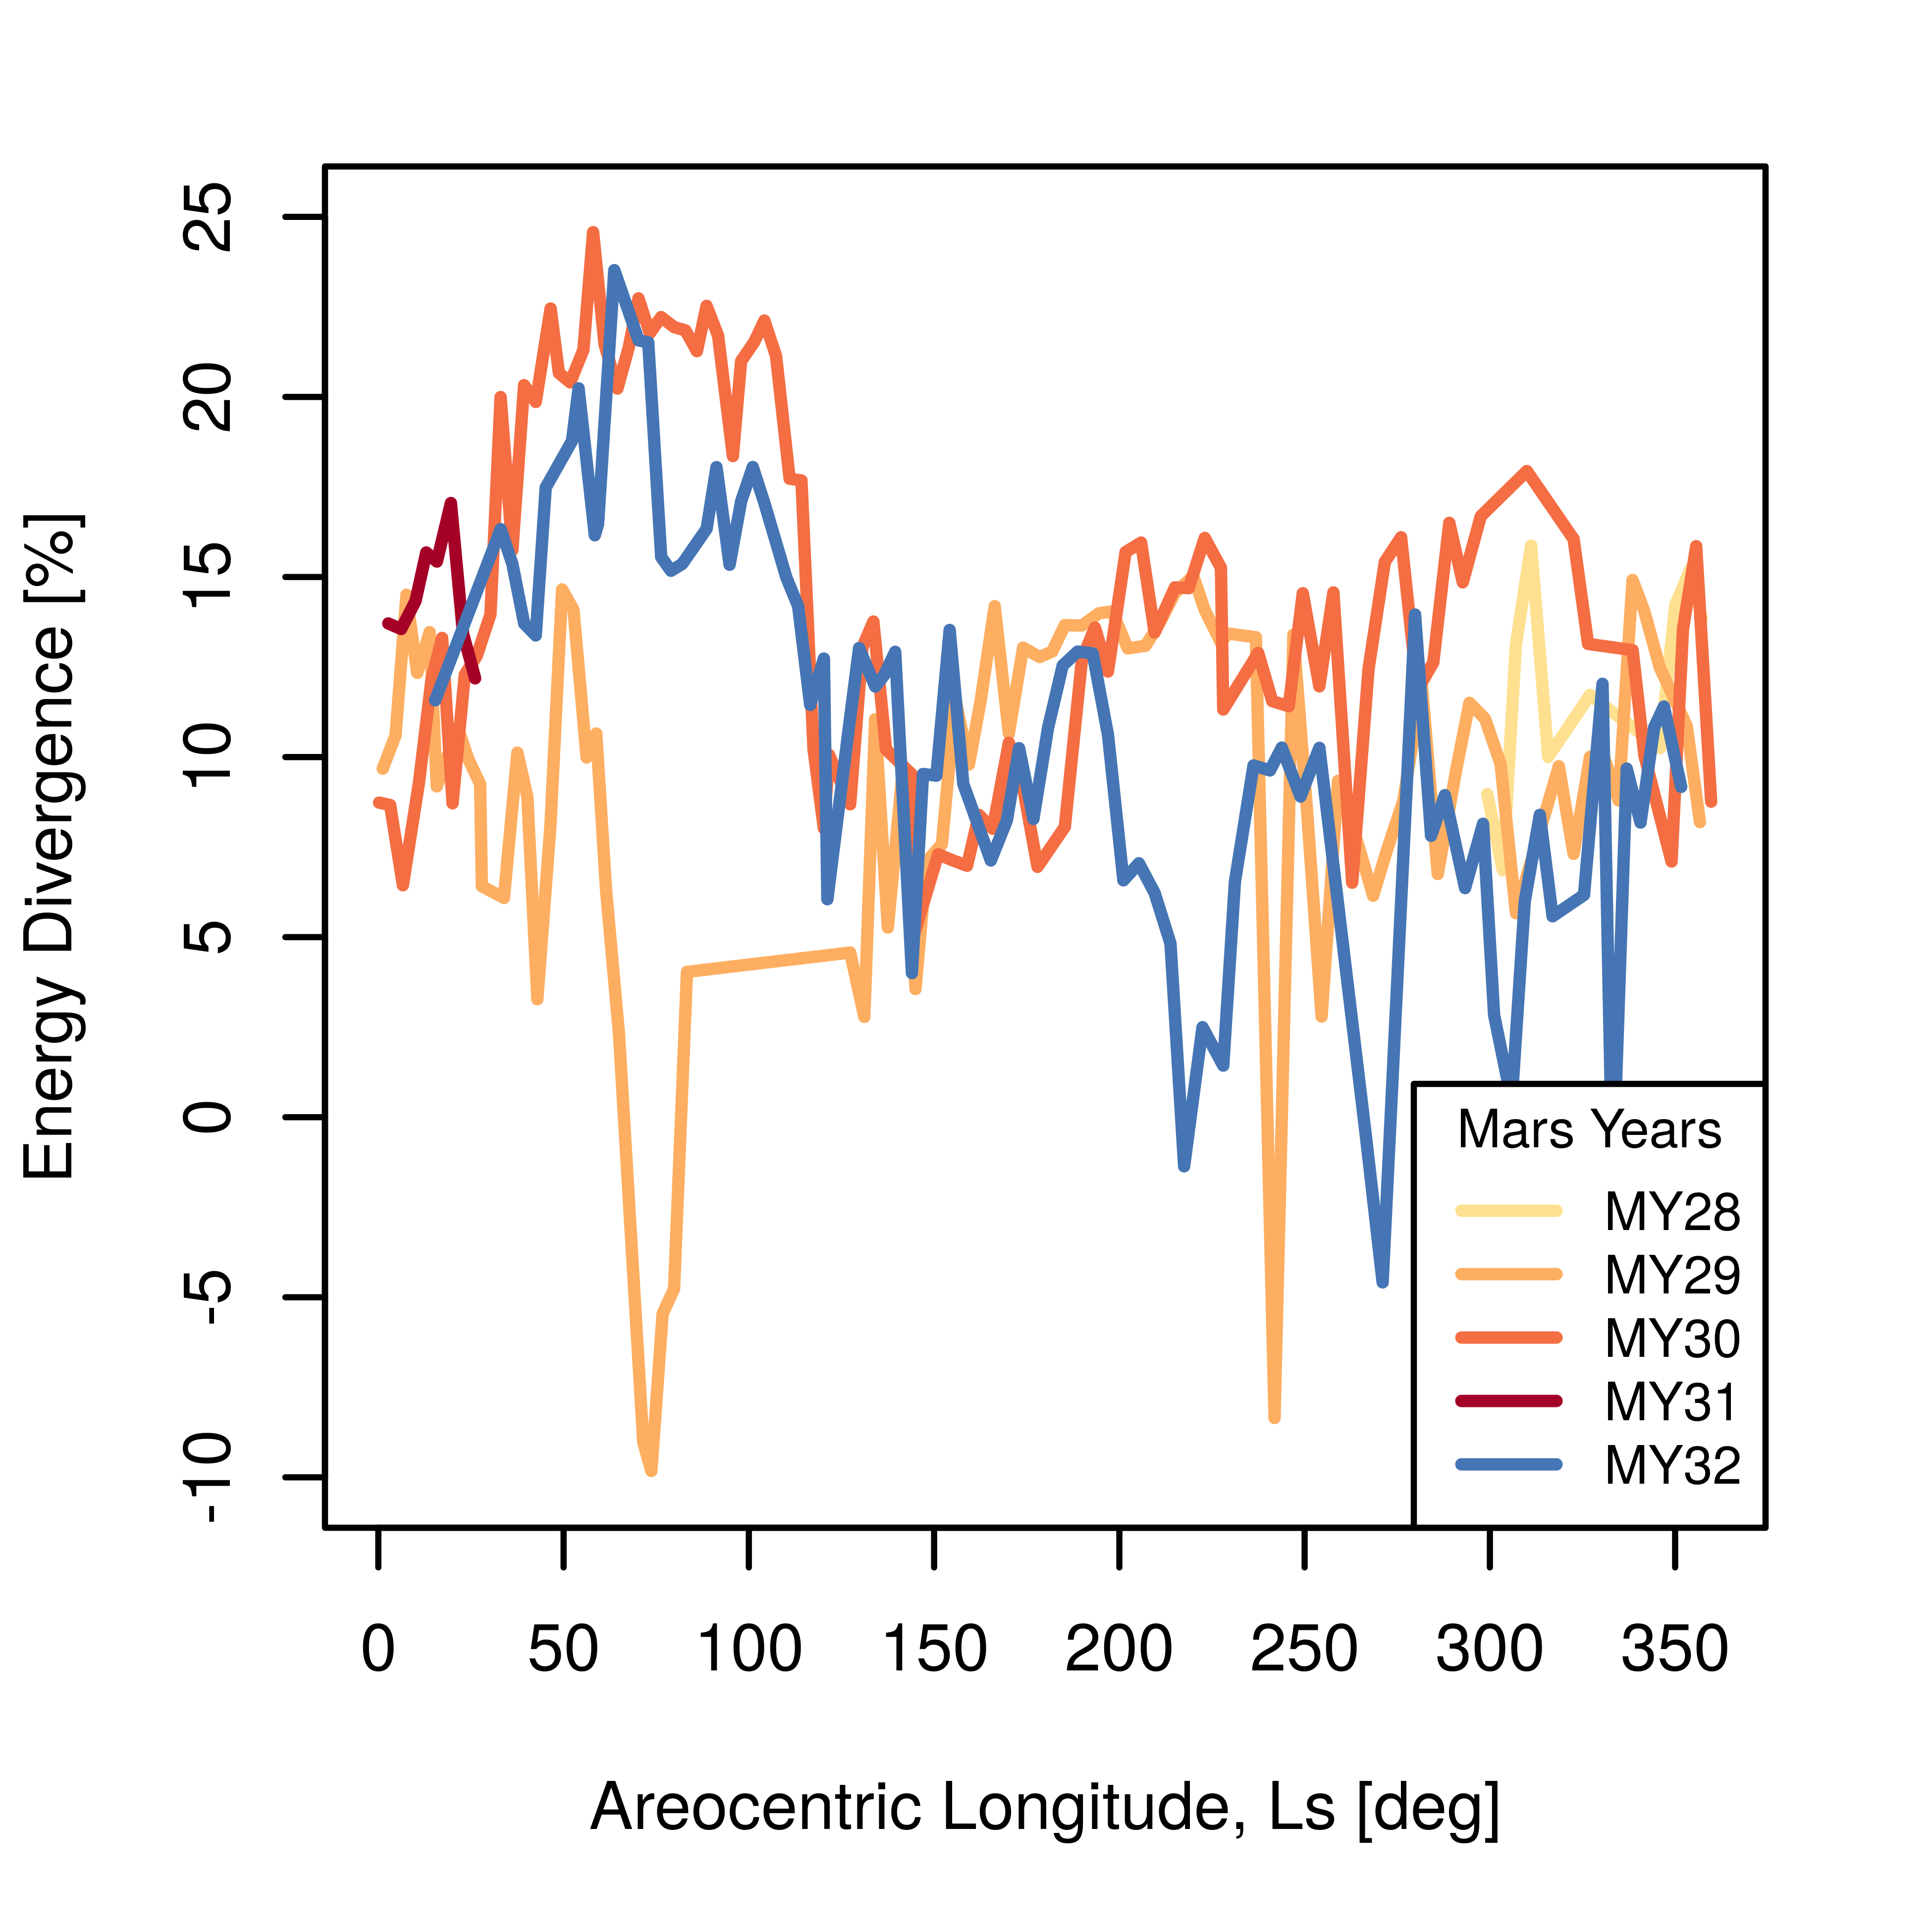
\includegraphics[width=0.8\linewidth]{sections/appendix/B/plots/energy-prediction-divergences-from-my28-to-my32-adjusted.png}\\
  \caption[Adjusted divergences from measured MER Opportunity PV energy production]
          {Adjusted divergences from measured MER Opportunity PV energy production.}
  \label{fig:plot:mer-energy-prediction-divergences-adjusted}
\end{figure}

\clearpage

\section{Ignoring Outliers}
\label{sec:Appendix:NarrowedEnergyPredictionErrorMarginRange:IgnoringOutliers}
In Figure \ref{fig:plot:binned-error-margins}, divergences greater than 5\% and lesser than -15\% were obtained with only 9.2\% of the dataset. With this in consideration, the process described in Section \ref{sec:Appendix:NarrowedEnergyPredictionErrorMarginRange:PreservingOutliers} was repeated without the data points responsible for the divergence outliers. This further narrowed down the error margin range to -11\%/+5\% by applying solar array dust factor adjustment of 5.4\% coupled with shadowing and other losses of 5\%. The resulting adjusted divergences are presented in Figure \ref{fig:plot:mer-energy-prediction-divergences-adjusted-without-outliers}:

\begin{figure}[h]
  \centering
  \hypersetup{linkcolor=captionTextColor}
  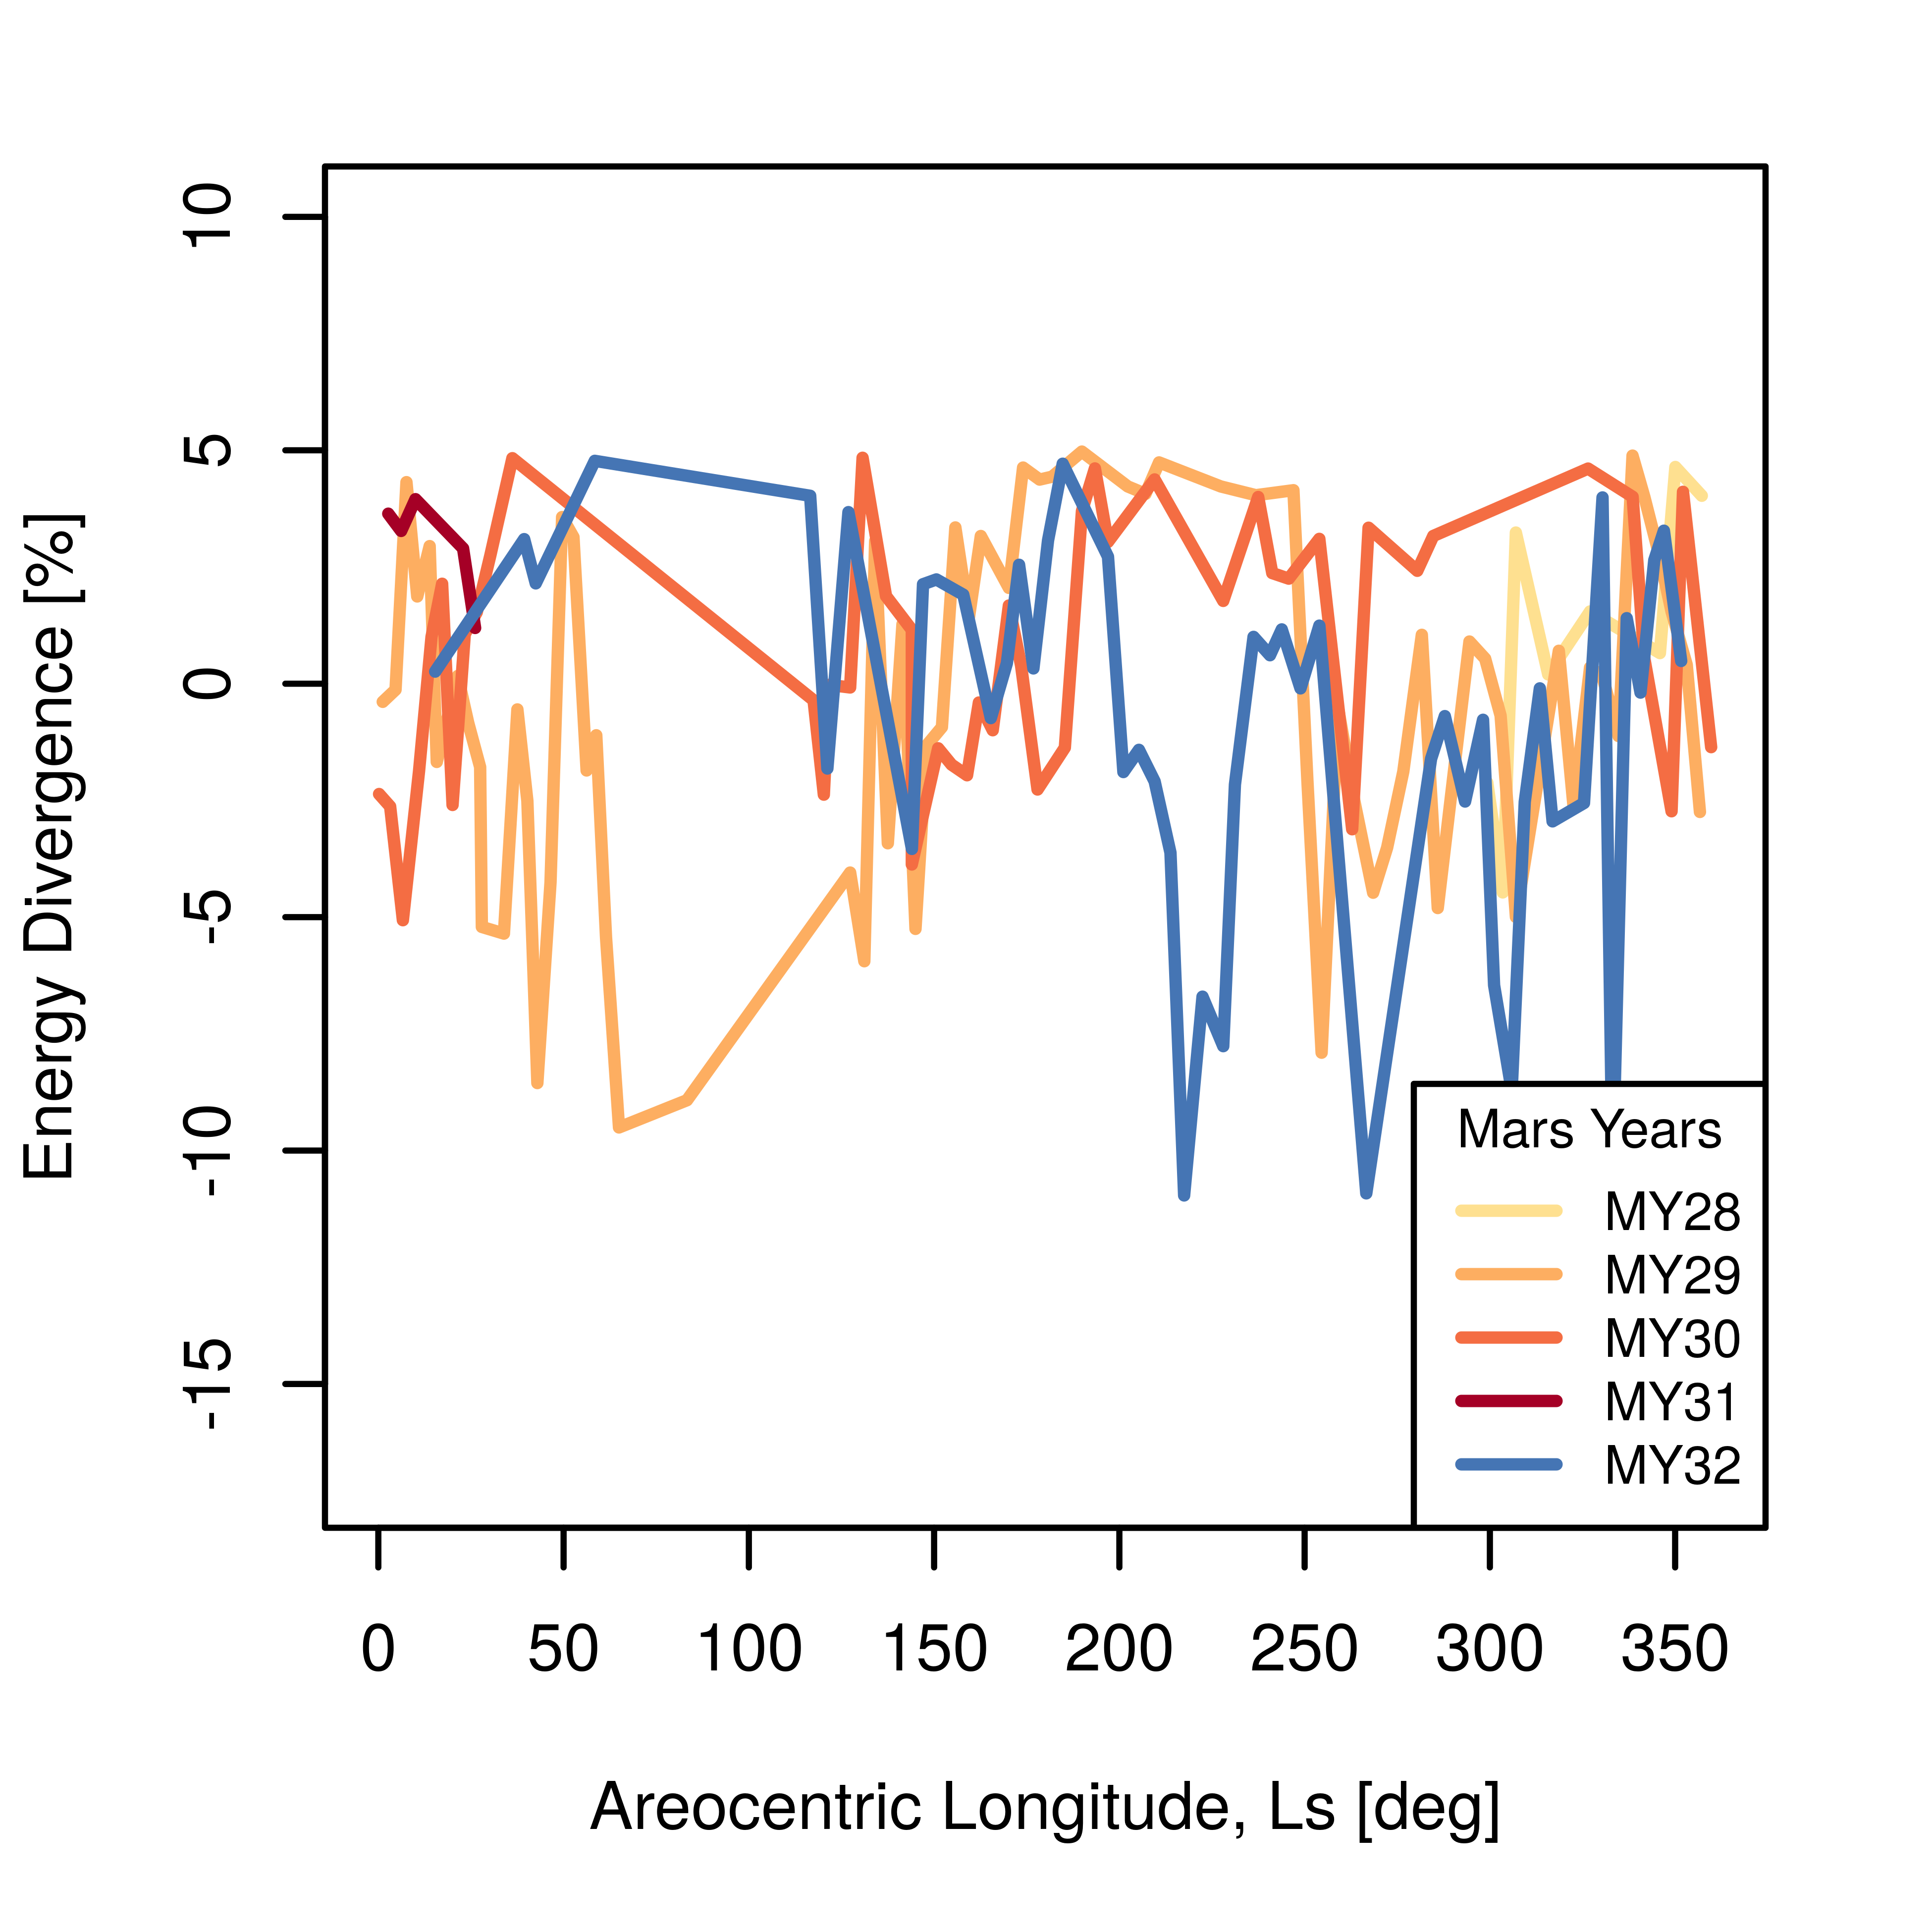
\includegraphics[width=0.8\linewidth]{sections/appendix/B/plots/energy-prediction-divergences-from-my28-to-my32-adjusted-without-outliers.png}\\
  \caption[Adjusted Outlierless divergences from measured MER Opportunity PV energy production]
          {Adjusted Outlierless divergences from measured MER Opportunity PV energy production.}
  \label{fig:plot:mer-energy-prediction-divergences-adjusted-without-outliers}
\end{figure}

\clearpage

\section{Conclusion}
\label{sec:Appendix:NarrowedEnergyPredictionErrorMarginRange:Conclusion}
The predicted generated energy curves in Figures \ref{fig:plot:sub:mer-energy-production-predicted-vs-reported-my29-adjusted}, \ref{fig:plot:sub:mer-energy-production-predicted-vs-reported-my30-adjusted}, and \ref{fig:plot:sub:mer-energy-production-predicted-vs-reported-my32-adjusted} were obtained through the process described in Section \ref{sec:Appendix:NarrowedEnergyPredictionErrorMarginRange:PreservingOutliers}. This resulted in overly conservative predictions when compared with the curve representing energy productions reported by MER Opportunity.

Predictions in Figures \ref{fig:plot:sub:mer-energy-production-predicted-vs-reported-my29-adjusted-without-outliers}, \ref{fig:plot:sub:mer-energy-production-predicted-vs-reported-my30-adjusted-without-outliers}, and \ref{fig:plot:sub:mer-energy-production-predicted-vs-reported-my32-adjusted-without-outliers} were obtained through the process described in Section \ref{sec:Appendix:NarrowedEnergyPredictionErrorMarginRange:IgnoringOutliers}. This resulted in predictions that more closely follow reported energy productions. Comparing these predictions with the unadjusted ones presented in Figure \ref{fig:plot:mer-energy-production-predicted-vs-reported} shows little changes and therefor do not justify the need to narrow down the error margin range for the purposes of preliminary mission scenario analysis.

\begin{figure}[h]
\captionsetup[subfigure]{justification=centering}
\vspace{-2ex}
	\centering
    %% setup sizes
    \setlength{\subfigureWidth}{0.32\textwidth}
    \setlength{\graphicsHeight}{50mm}
    %% kill hyper-link highlighting
    \hypersetup{hidelinks=true}%
    %% the figures
	\begin{subfigure}[t]{\subfigureWidth}
        \centering
		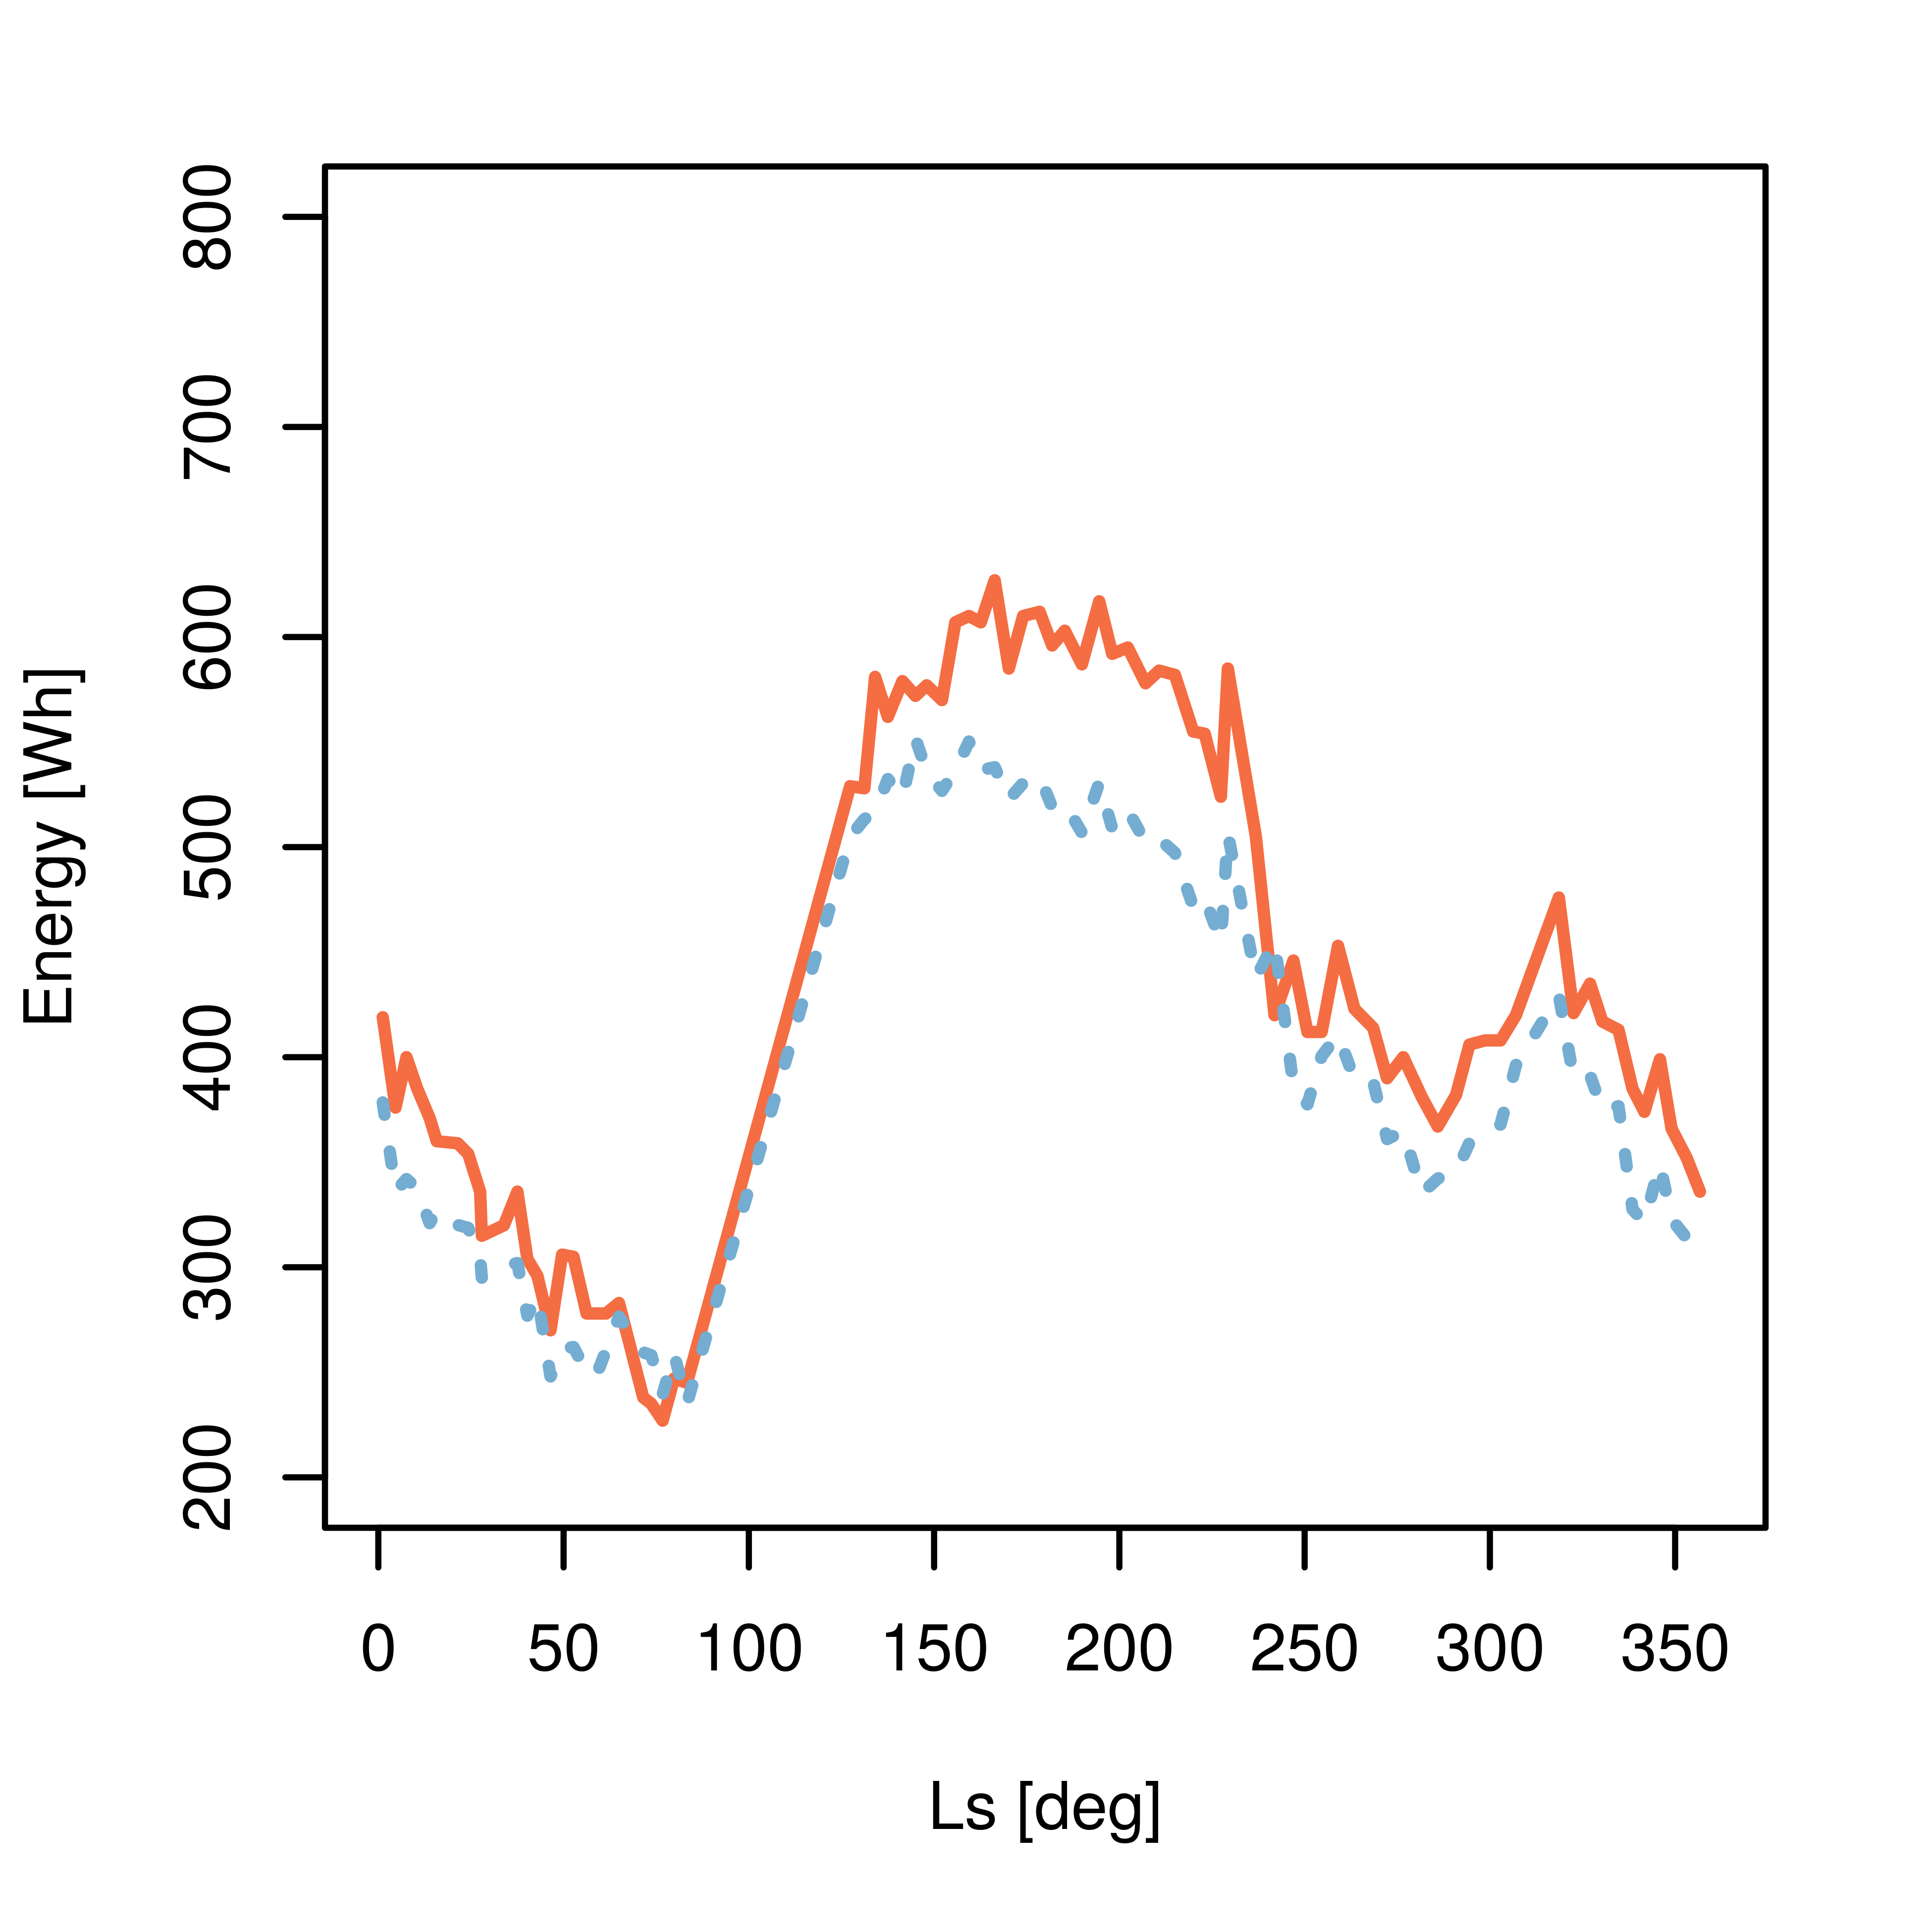
\includegraphics[height=\graphicsHeight]{sections/appendix/B/plots/predicted-vs-measured-energy-my29-adjusted.png}
		\subcaption{MY29}
		\label{fig:plot:sub:mer-energy-production-predicted-vs-reported-my29-adjusted}
	\end{subfigure}\hfill
	\begin{subfigure}[t]{\subfigureWidth}
        \centering
		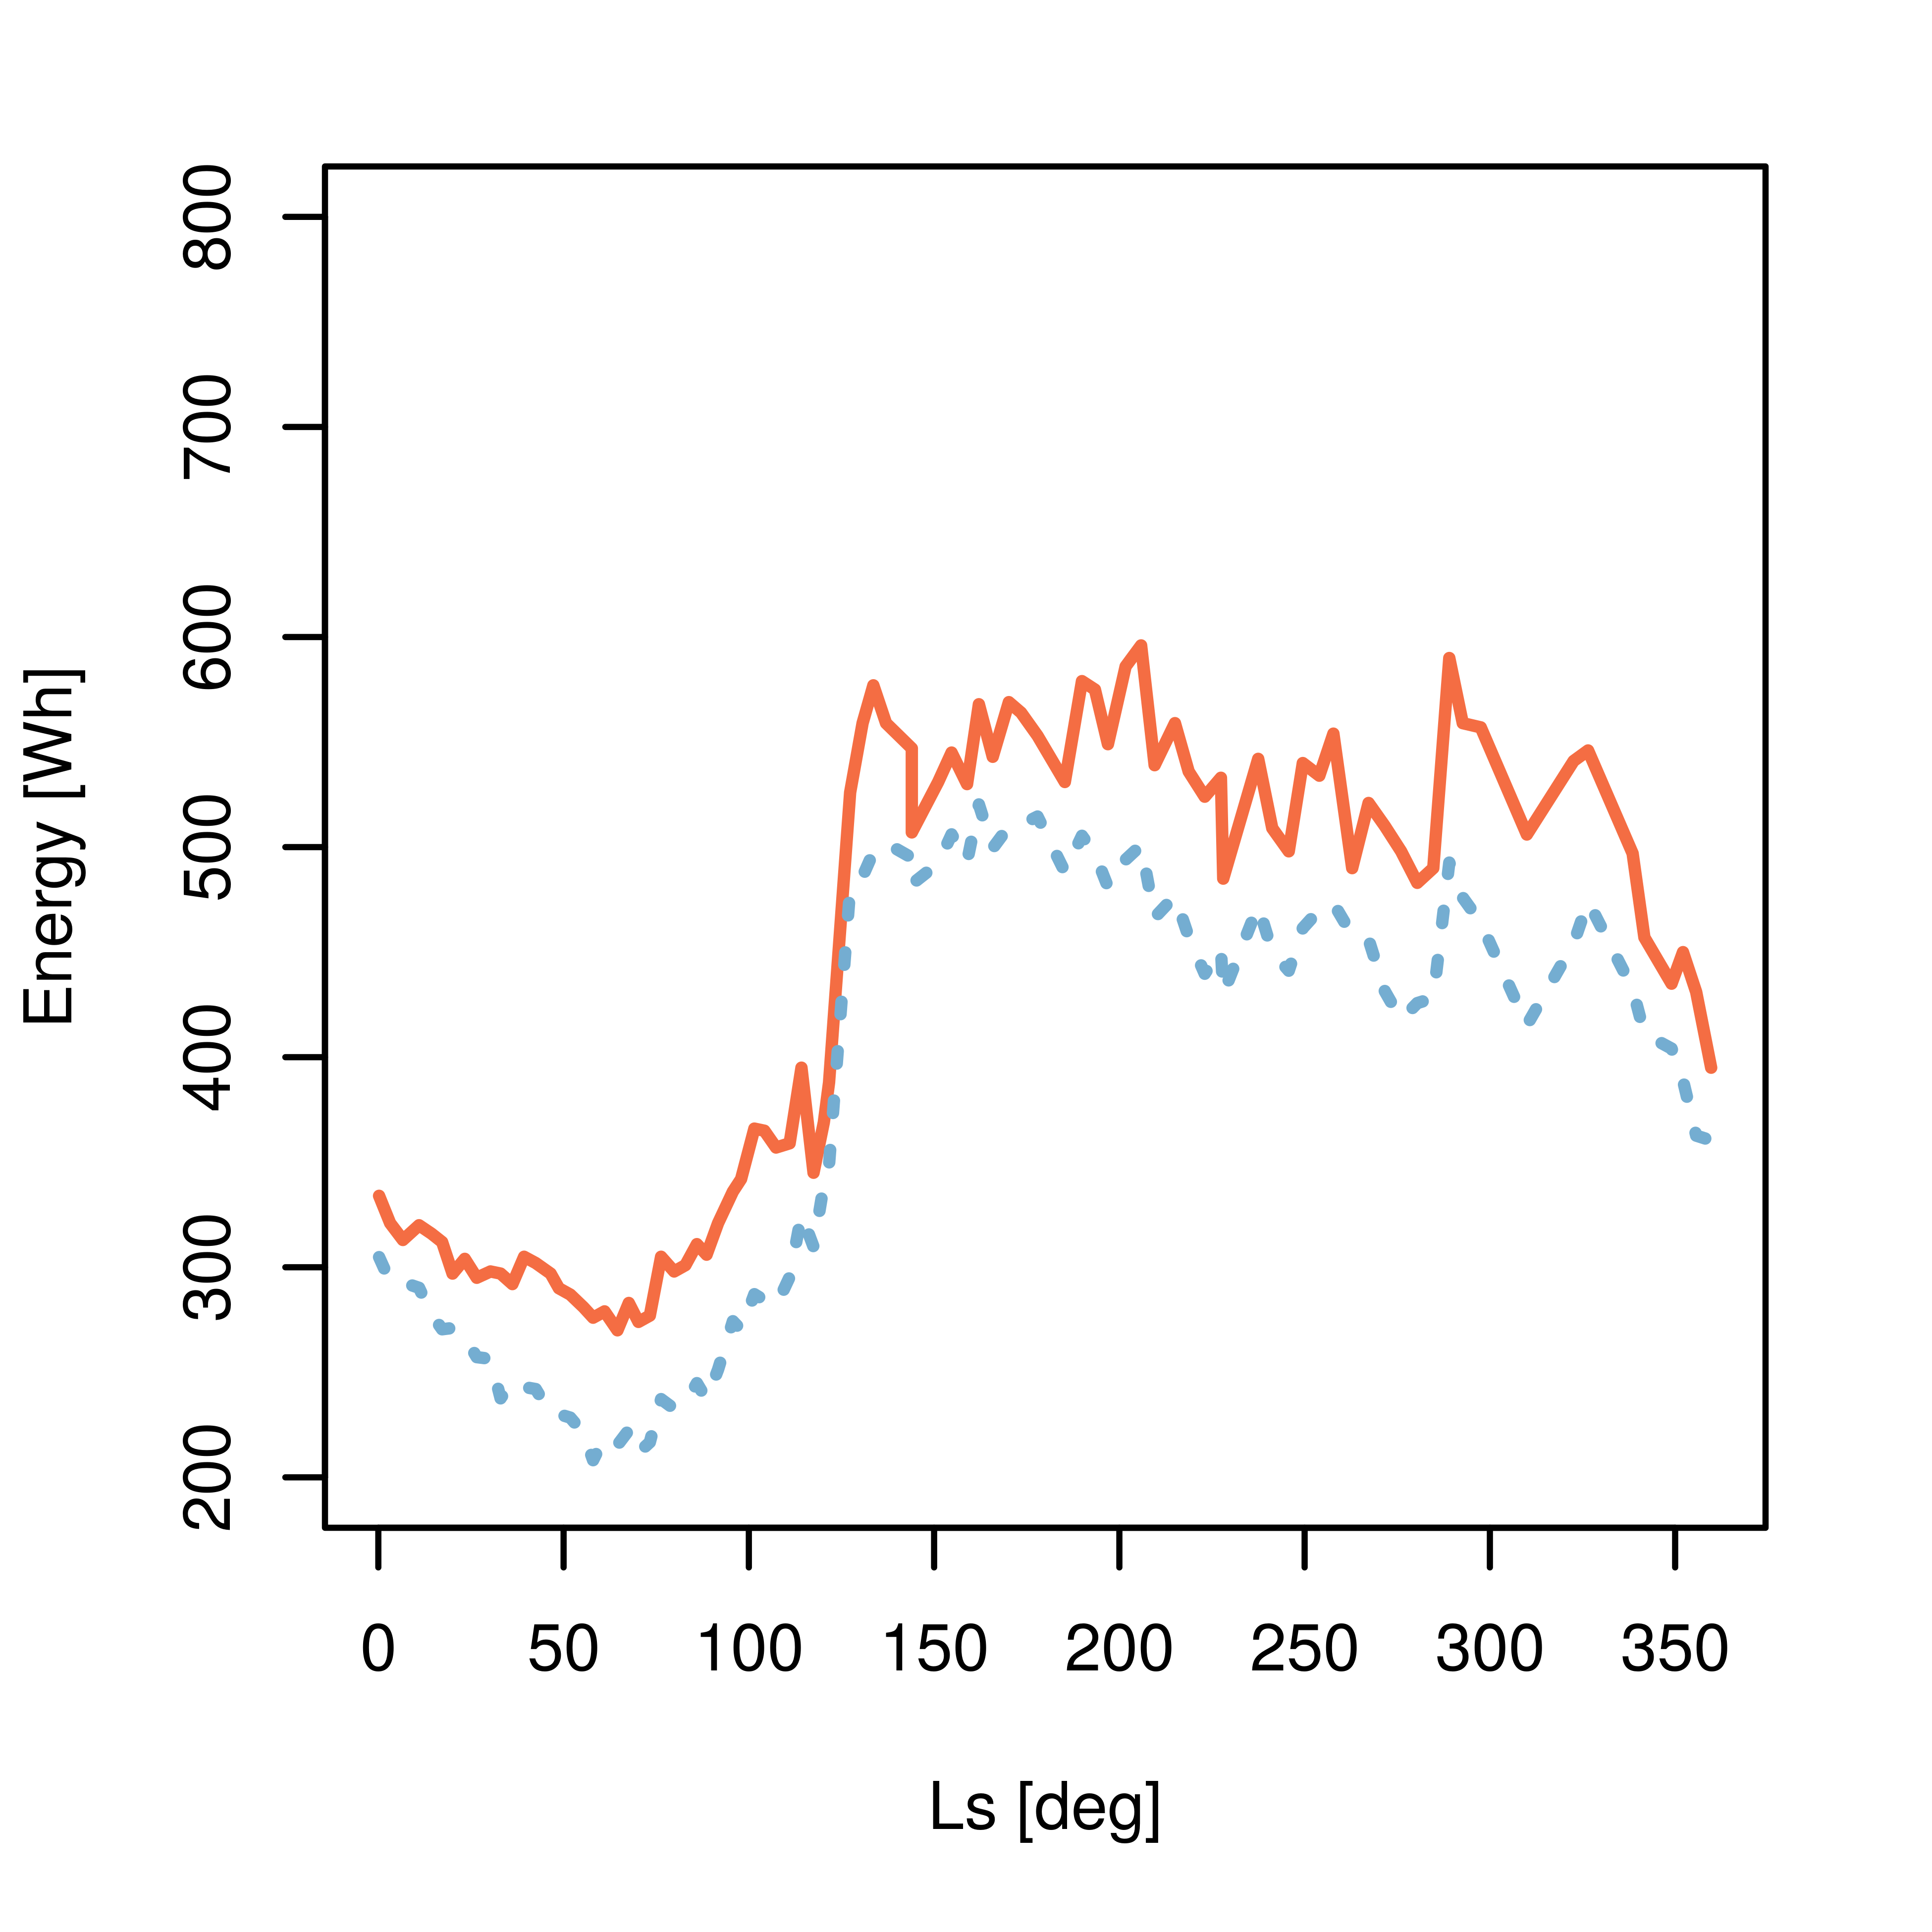
\includegraphics[height=\graphicsHeight]{sections/appendix/B/plots/predicted-vs-measured-energy-my30-adjusted.png}
		\subcaption{MY30}
		\label{fig:plot:sub:mer-energy-production-predicted-vs-reported-my30-adjusted}
	\end{subfigure}\hfill
    \begin{subfigure}[t]{\subfigureWidth}
        \centering
		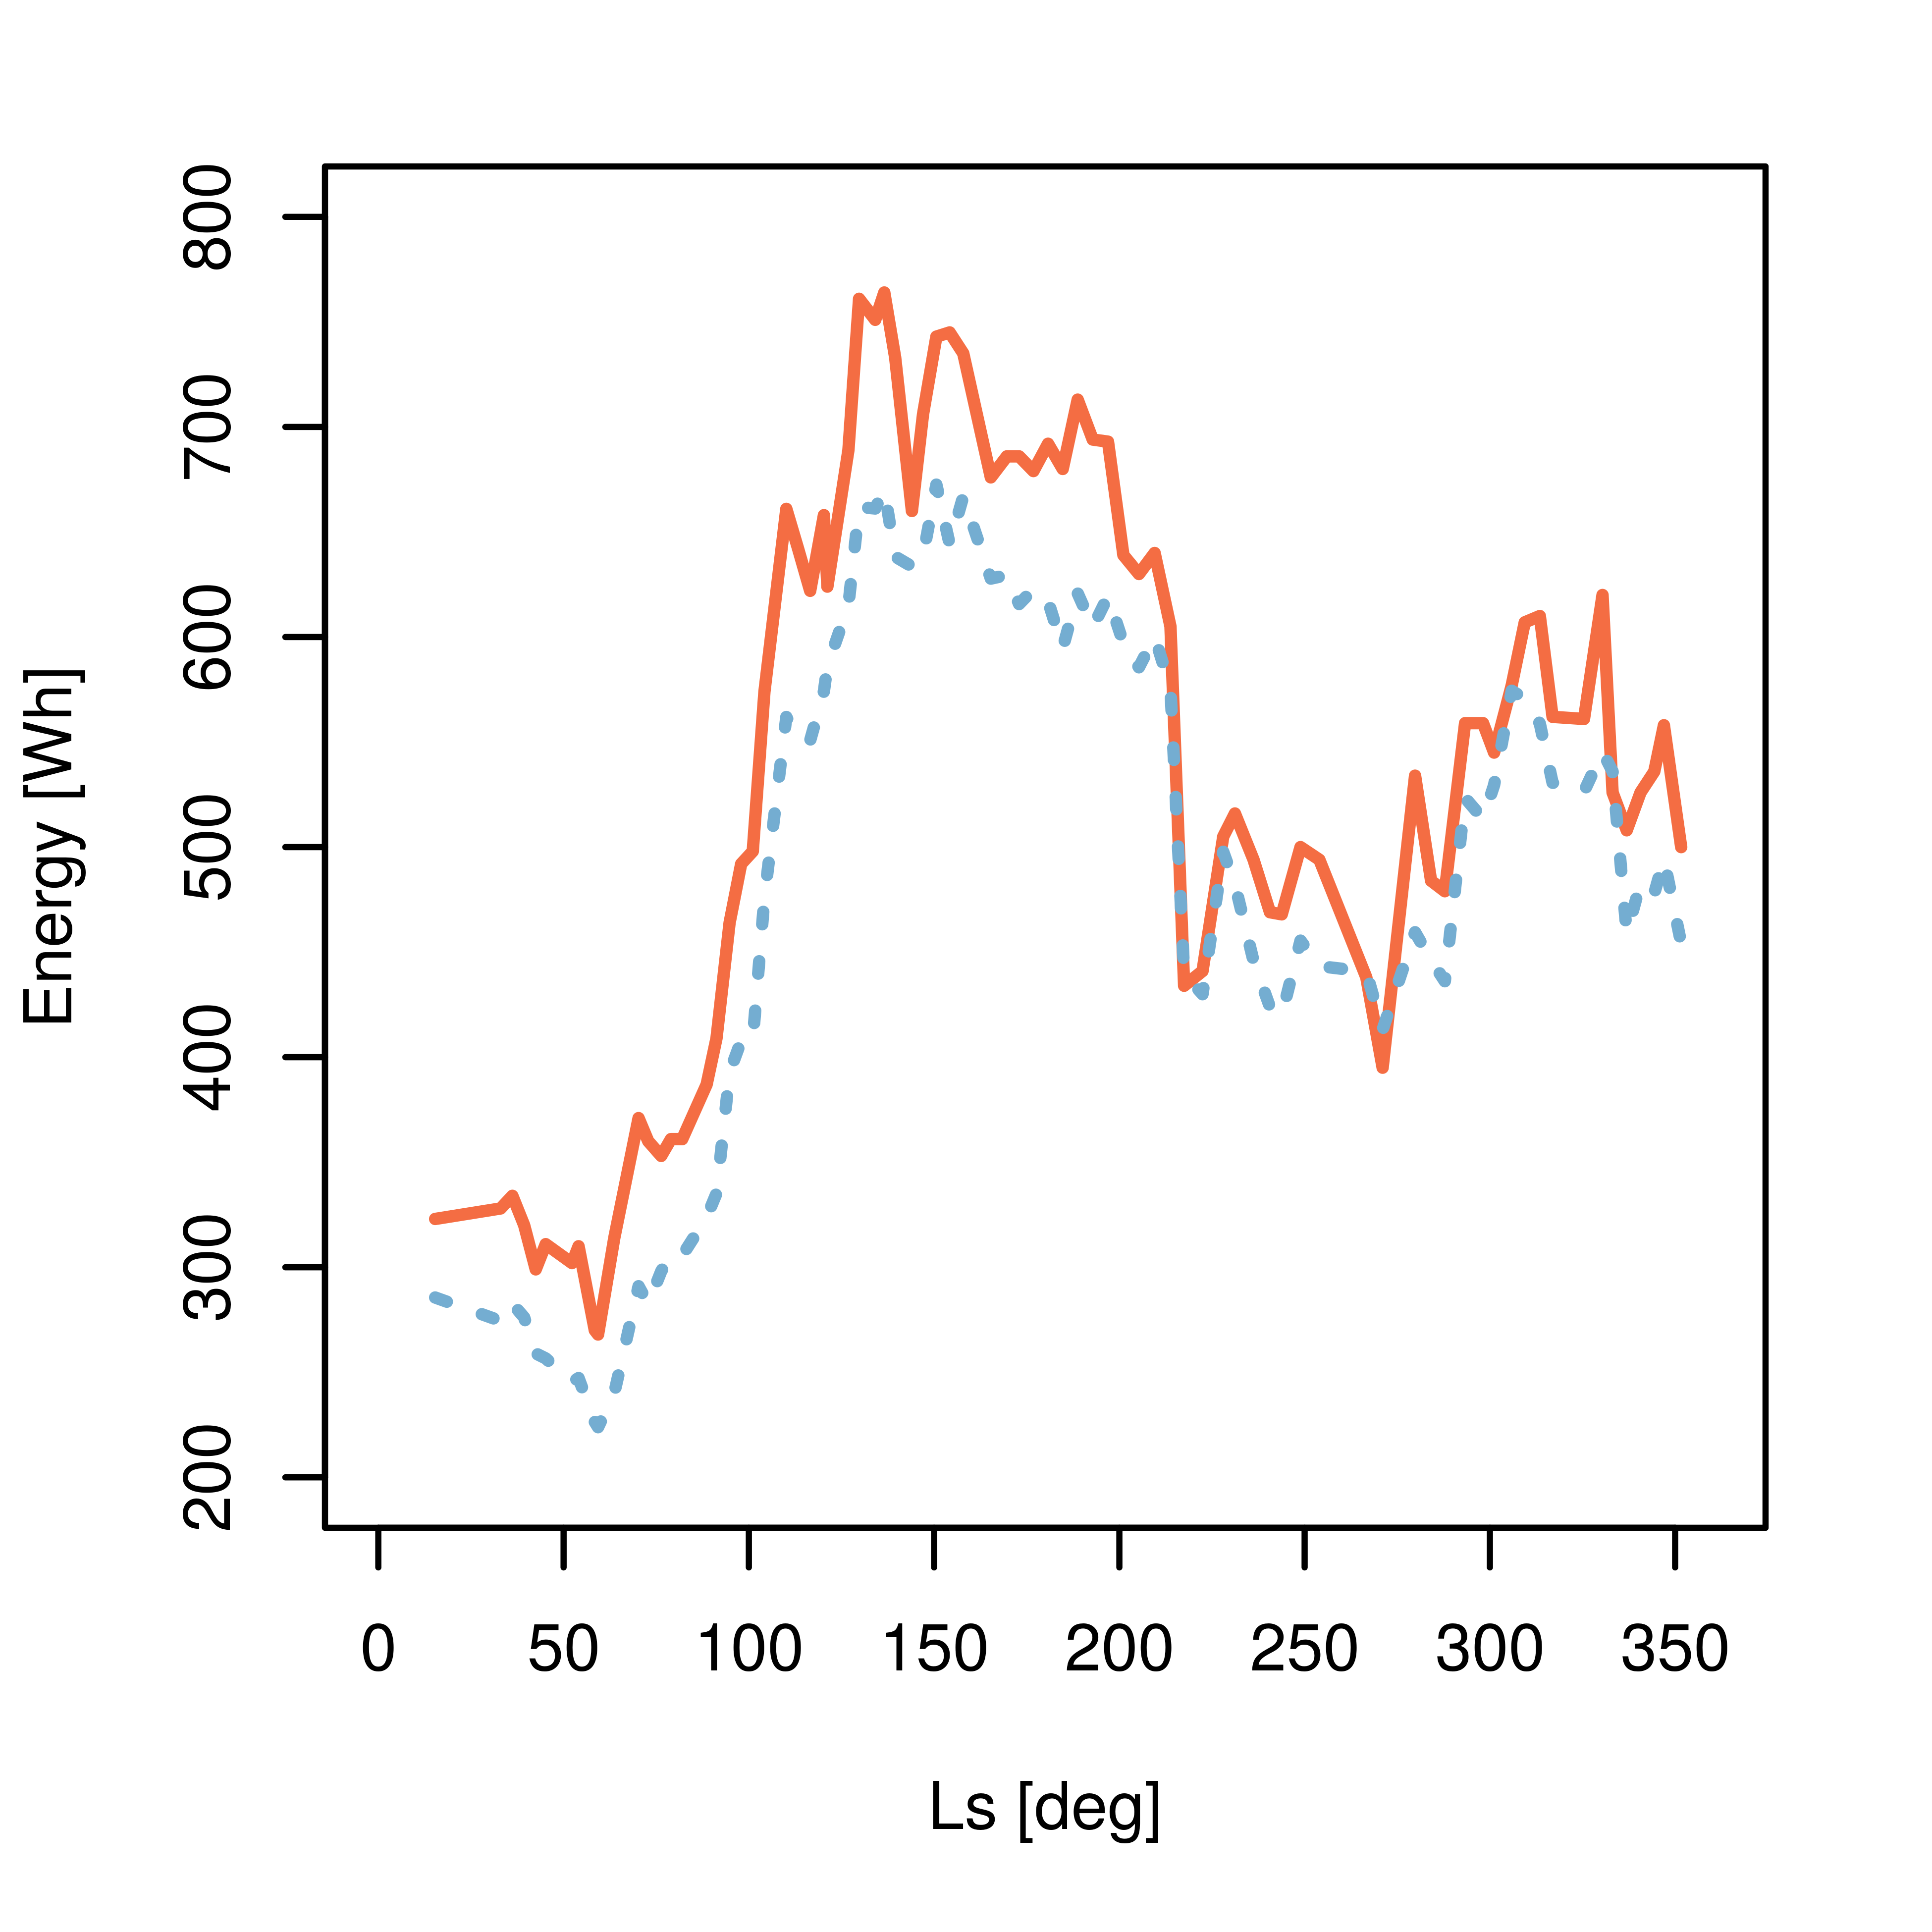
\includegraphics[height=\graphicsHeight]{sections/appendix/B/plots/predicted-vs-measured-energy-my32-adjusted.png}
		\subcaption{MY32}
		\label{fig:plot:sub:mer-energy-production-predicted-vs-reported-my32-adjusted}
	\end{subfigure}\\[0.8ex]
%% 2nd row
    \begin{subfigure}[t]{\subfigureWidth}
        \centering
		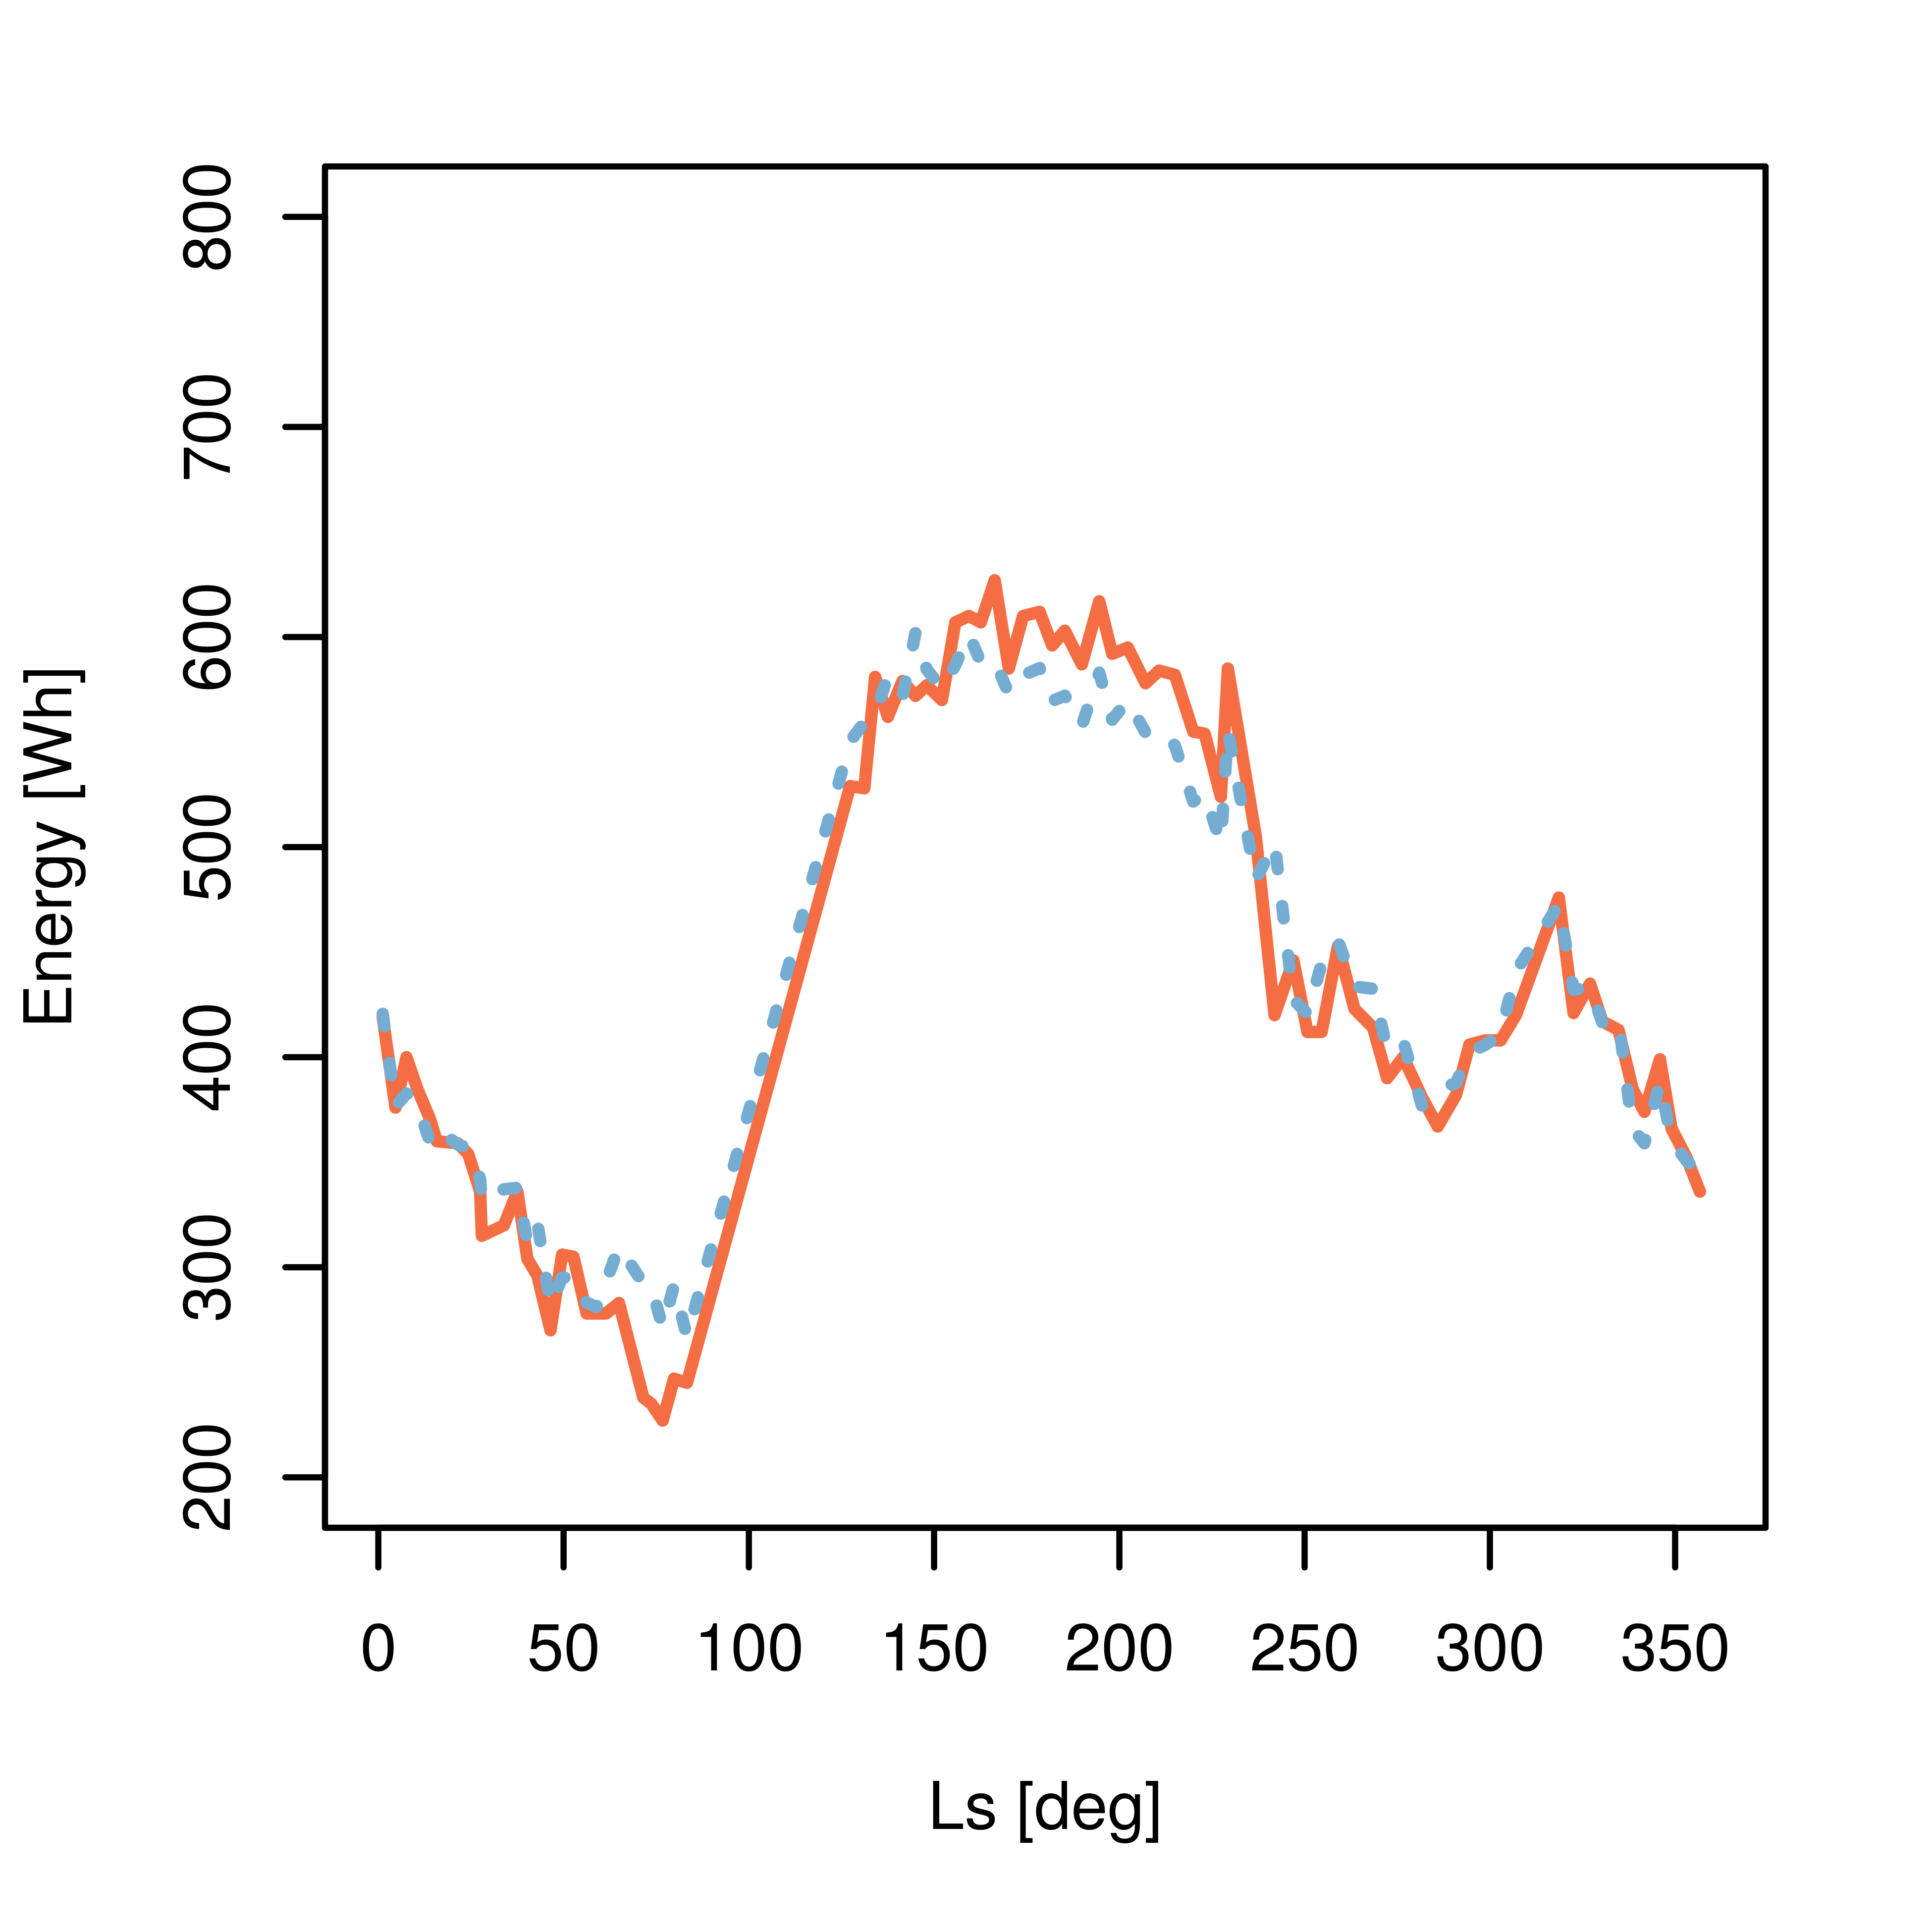
\includegraphics[height=\graphicsHeight]{sections/appendix/B/plots/predicted-vs-measured-energy-my29-adjusted-without-outliers.png}
		\subcaption{MY29}
		\label{fig:plot:sub:mer-energy-production-predicted-vs-reported-my29-adjusted-without-outliers}
	\end{subfigure}\hfill
	\begin{subfigure}[t]{\subfigureWidth}
        \centering
		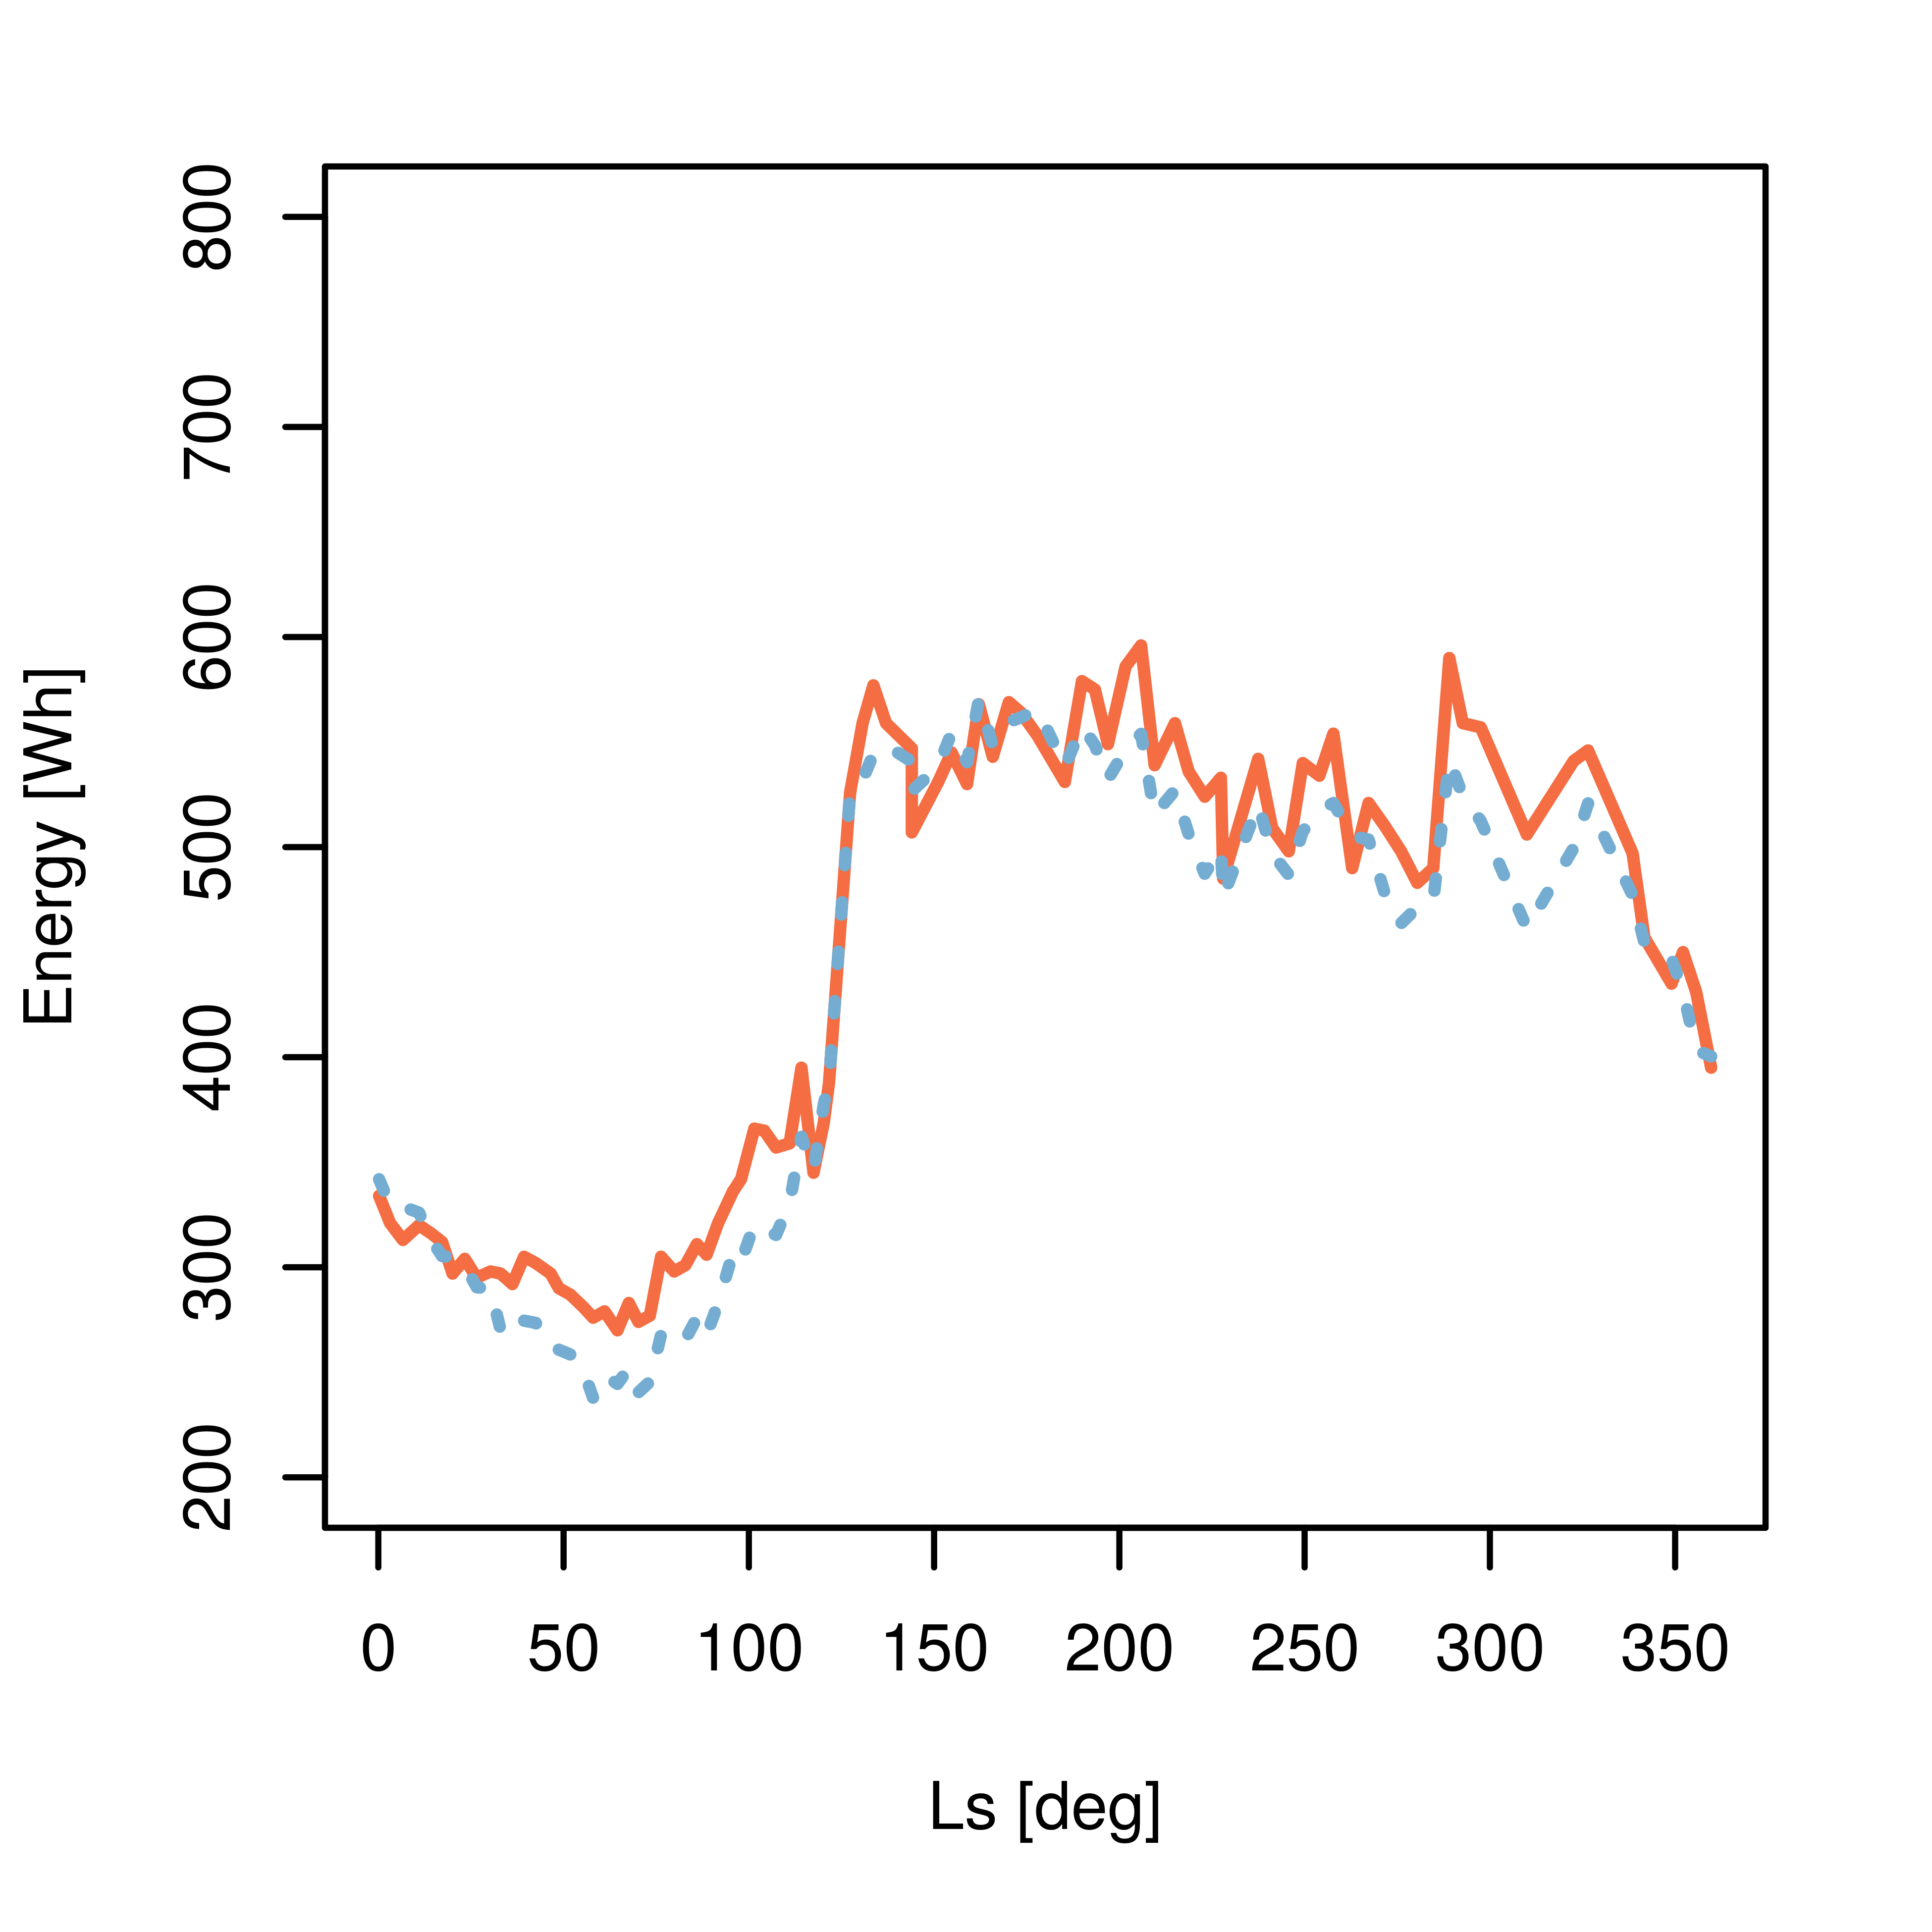
\includegraphics[height=\graphicsHeight]{sections/appendix/B/plots/predicted-vs-measured-energy-my30-adjusted-without-outliers.png}
		\subcaption{MY30}
		\label{fig:plot:sub:mer-energy-production-predicted-vs-reported-my30-adjusted-without-outliers}
	\end{subfigure}\hfill
    \begin{subfigure}[t]{\subfigureWidth}
        \centering
		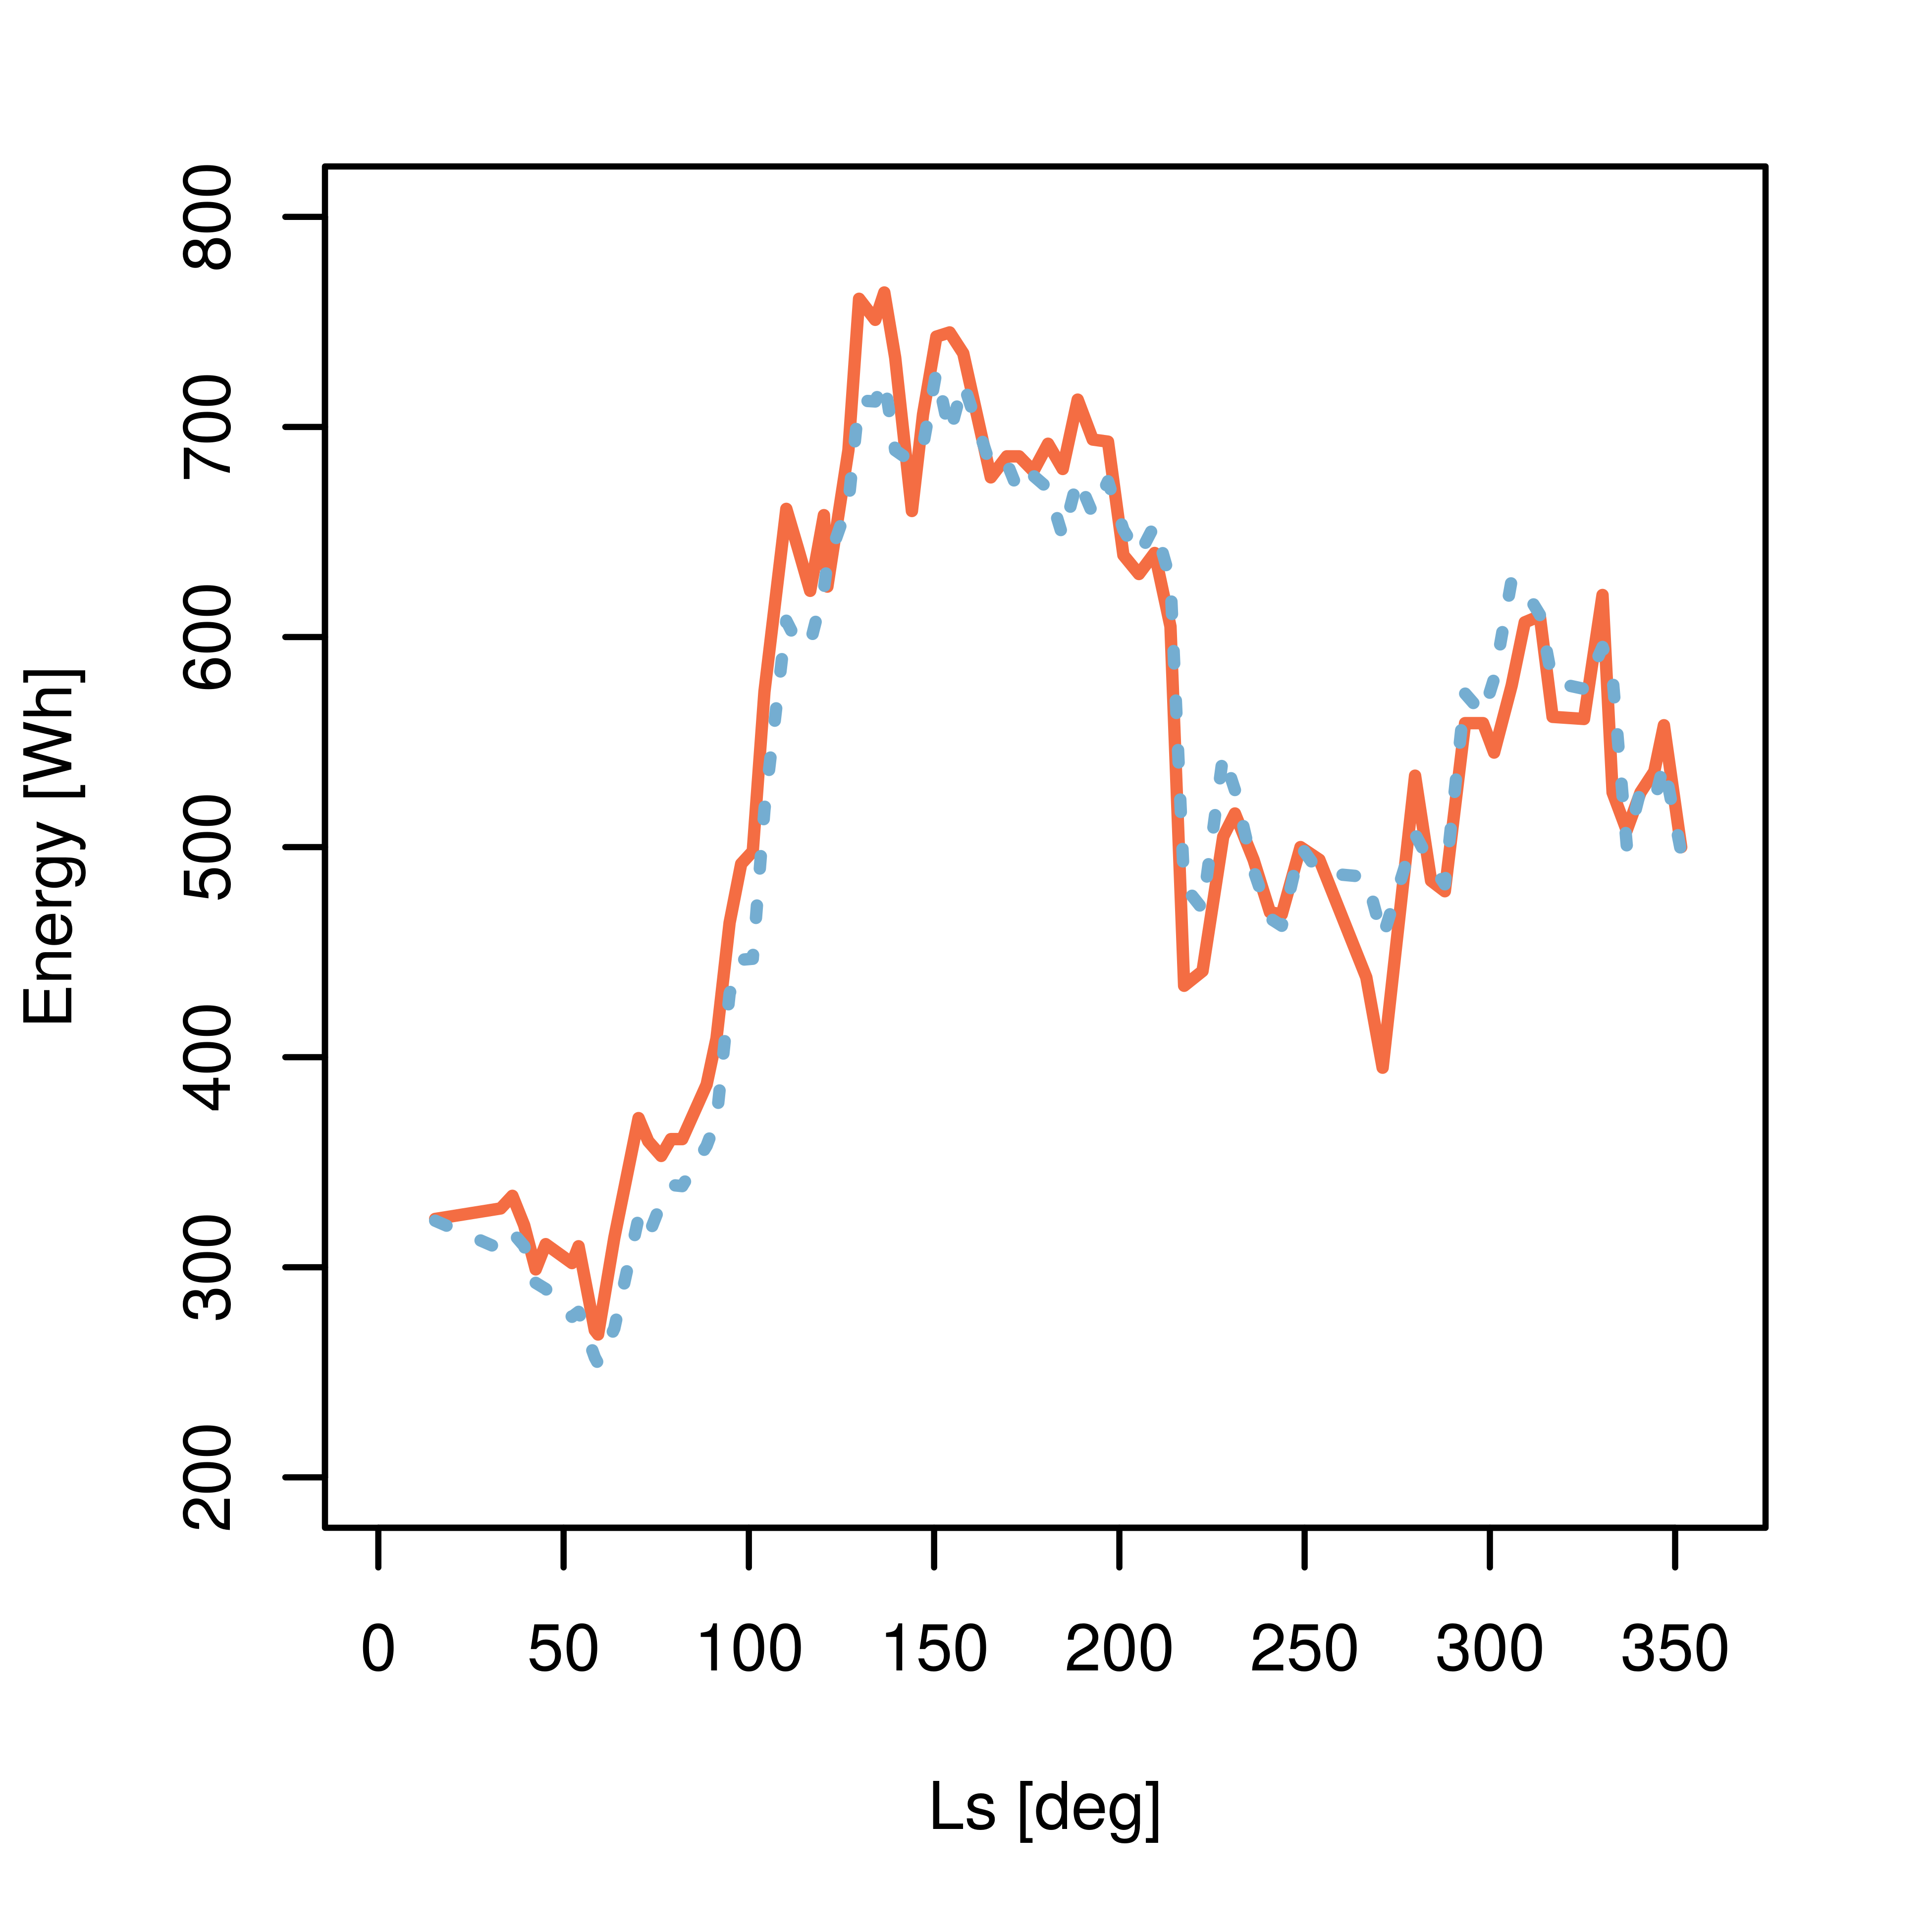
\includegraphics[height=\graphicsHeight]{sections/appendix/B/plots/predicted-vs-measured-energy-my32-adjusted-without-outliers.png}
		\subcaption{MY32}
		\label{fig:plot:sub:mer-energy-production-predicted-vs-reported-my32-adjusted-without-outliers}
	\end{subfigure}
    \caption[\ac{MER} Opportunity \ac{PV} energy production: adjusted prediction vs reported]
            {\ac{MER} Opportunity \ac{PV} energy production: adjusted prediction vs reported. The predicted lines across the first row were obtained with iteratively determined calculation adjustments that narrowed the calculated predicted values' error margin range from -33\%/+7\% to -10\%/+25\%. The second row was obtain in a similar fashion but with outlier divergences ignored which further narrowed the error margin range to -11\%/+5\%.}
    \label{fig:plot:mer-energy-production-predicted-vs-reported-adjusted-with-and-without-outliers}
\vspace{-2ex}
\end{figure}

\clearpage


%\addcontentsline{toc}{chapter}{Accumulated Publications}
%#%\chapter{More Stuff}
%#%\label{sec:Appendix:MoreStuff}


%% this is how to teak the toc:
%% add extra spacing to get caption on next page of toc
%\cftaddtitleline{toc}{chapter}{\vspace{5mm}}{} %extra neg. space in toc

%#%\chapter{Enough!}
%#%\label{sec:Appendix:Enough}

%#%\end{appendix}



\end{document}
